%%%%%%%%%%%%%%%%%%%%%%%%
%% Sample use of the infthesis class to prepare a thesis. This can be used as 
%% a template to produce your own thesis.
%%
%% The title, abstract and so on are taken from Martin Reddy's csthesis class
%% documentation.
%%
%% MEF, October 2002
%%%%%%%%%%%%%%%%%%%%%%%%

%%%%
%% Load the class. Put any options that you want here (see the documentation
%% for the list of options). The following are samples for each type of
%% thesis:
%%
%% Note: you can also specify any of the following options:
%%  logo: put a University of Edinburgh logo onto the title page
%%  frontabs: put the abstract onto the title page
%%  deptreport: produce a title page that fits into a Computer Science
%%      departmental cover [not sure if this actually works]
%%  singlespacing, fullspacing, doublespacing: choose line spacing
%%  oneside, twoside: specify a one-sided or two-sided thesis
%%  10pt, 11pt, 12pt: choose a font size
%%  centrechapter, leftchapter, rightchapter: alignment of chapter headings
%%  sansheadings, normalheadings: headings and captions in sans-serif
%%      (default) or in the same font as the rest of the thesis
%%  [no]listsintoc: put list of figures/tables in table of contents (default:
%%      not)
%%  romanprepages, plainprepages: number the preliminary pages with Roman
%%      numerals (default) or consecutively with the rest of the thesis
%%  parskip: don't indent paragraphs, put a blank line between instead
%%  abbrevs: define a list of useful abbreviations (see documentation)
%%  draft: produce a single-spaced, double-sided thesis with narrow margins
%%
%% For a PhD thesis -- you must also specify a research institute:
%\documentclass[phd,ilcc,twoside]{infthesis}
\documentclass[mscres,icsa,logo,twoside]{infthesis}

%% For an MPhil thesis -- also needs an institute
% \documentclass[mphil,ianc]{infthesis}

%% MSc by Research, which also needs an institute
% \documentclass[mscres,irr]{infthesis}

%% Taught MSc -- specify a particular degree instead. If none is specified,
%% "MSc in Informatics" is used.
% \documentclass[msc,cogsci]{infthesis}
% \documentclass[msc]{infthesis}  % for the MSc in Informatics

%% Master of Informatics (5 year degree)


%% Logo Style: University of Edinburgh Shield
% \documentclass[minf]{infthesis}
%% Possible values for shieldtype:
%% 0: regular monochrome
%% 1: monochrome with no background lines
%% 2: reverse monochrome
%% 3: two colours: navy and red
%% 4: full colour
\shieldtype{4}

%% Undergraduate project -- specify the degree course and project type
%% separately
% \documentclass[bsc]{infthesis}
% \course{Artificial Intelligence and Psychology}
% \project{Fourth Year Project Report}

%% Put any \usepackage commands you want to use right here; the following is 
%% an example:
\usepackage{natbib}


\usepackage{float}

\usepackage{graphics}

\usepackage{graphicx}
\usepackage{subcaption}

%\usepackage{setspace}
\usepackage{ragged2e}


\usepackage{amsthm}
\usepackage{amsmath,amssymb}
%\usepackage{mathrsfs}
\usepackage{mathtools}

\theoremstyle{definition}
\newtheorem{definition}{Definition}[section]
\newtheorem{prop}{Proposition}[section]

\usepackage[noend]{algpseudocode}
\usepackage{algorithm}


\newcommand{\etal}{et~al.}

\newcommand{\itercomp}{{iterative compilation}}
\newcommand{\Itercomp}{{Iterative compilation}}
\newcommand{\IterComp}{{Iterative Compilation}}

\usepackage{multirow}


%% Listing related stuff
\usepackage{listings}
\usepackage{courier}            %Required for pretty listings (more dense)

\usepackage[table]{xcolor}

%% EMACS colors for listing:
\usepackage{color}
\definecolor{sh_comment}{rgb}{0.65, 0.00, 0.00 } % red-ish
\definecolor{sh_keyword}{rgb}{0.37, 0.69, 0.69}  % blue-green
\definecolor{sh_string}{rgb}{0.08, 0.69, 0.08} % green

%% This manipulates the listing numbering. It decreases it by one at the point used.
\newcommand*\lstDNumber{\addtocounter{lstnumber}{-1}}

%% Change from Listing->Algorithm
%% \renewcommand\lstlistingname{Algorithm} % Fix listing caption name: Listing -> Algorithm
%% \renewcommand\lstlistlistingname{Algorithms}
%% \def\lstlistingautorefname{Alg.}

%% \renewcommand{\thelstlisting}{\thesection-\arabic{lstlisting}}
%\renewcommand{\thelstlisting}{\arabic{lstlisting}} % Fix listing numbering Algorithm 1.1 -> Algorithm 1.

%% \renewcommand{\labelenumi}{\roman{enumi}.}

\lstset{
float=[*],
language=C,                % choose the language of the code
%% basicstyle=\linespread{0.9}
%% basicstyle=\scriptsize\ttfamily,
 basicstyle={\linespread{0.97} \scriptsize\ttfamily},
 stringstyle=\color{sh_string},
 keywordstyle = \color{sh_keyword}\bfseries,
 commentstyle=\color{sh_comment}\itshape,
numbers=left,                   % where to put the line-numbers
%% numberstyle=\scriptsize,        % the size of the fonts that are used for the line-numbers
numberstyle=\scriptsize,        % the size of the fonts that are used for the line-numbers
stepnumber=1,                   % the step between two line-numbers. If it is 1 each line will be numbered
numbersep=5pt,                  % how far the line-numbers are from the code
backgroundcolor=\color{white},  % choose the background color. You must add \usepackage{color}
showspaces=false,               % show spaces adding particular underscores
showstringspaces=false,         % underline spaces within strings
showtabs=false,                 % show tabs within strings adding particular underscores
xleftmargin=2em,                % Left margin
frame=lines,                   % adds a frame around the code. none|leftline|topline|bottomline|lines|single|shadowbox
framexleftmargin=1.5em,         % Margin from frame to line numbers
framexbottommargin=0em,         % Distance from last text to frame
morekeywords={in,true,false,and,or,set},
%% prebreak=\mbox{\tiny$\searrow$},
prebreak=\space,                % Line break: insert this character at the end of the top line
%% postbreak=\mbox{{\color{blue}\scriptsize$\hookrightarrow$}}, % Line break: blue arrow at the beginning of the bottom line
postbreak=\mbox{{\color{blue}\scriptsize$\hookrightarrow$}}, % Line break: blue arrow at the beginning of the bottom line
breaklines=true,                % sets automatic line breaking
breakatwhitespace=false,        % sets if automatic breaks should only happen at whitespace
tabsize=2,                      % sets default tabsize to 2 spaces
captionpos=b,                   % sets the caption-position to top
%escapeinside={\@}{\@}             % Escape sequence \@ESCAPED STUFF\@
}

\usepackage{nasm/lang}
\usepackage{nasm/style}
\usepackage{llvm/lang}


%% Information about the title, etc.
\title{Online {\IterComp}\\Guided by Work-based Profiling}
\author{Rodrigo Caetano de Oliveira Rocha}

%% If the year of submission is not the current year, uncomment this line and 
%% specify it here:
% \submityear{1785}

%% Optionally, specify the graduation month and year:
% \graduationdate{February 1786}

%% Specify the abstract here.
\abstract{%

}

%% Now we start with the actual document.
\begin{document}

%% First, the preliminary pages
\begin{preliminary}

%% This creates the title page
\maketitle

%% Acknowledgements
\begin{acknowledgements}
%This work was supported in part by the EPSRC Centre for Doctoral Training in Pervasive Parallelism, funded by the UK Engineering and Physical Sciences Research Council (grant EP/L01503X/1) and the University of Edinburgh.

This work was supported in part by the EPSRC Centre for Doctoral Training in Pervasive Parallelism, funded by the UK Engineering and Physical Sciences Research Council (grant EP/L01503X/1) and the University of Edinburgh.
\end{acknowledgements}

%% Next we need to have the declaration.
\standarddeclaration

%% Finally, a dedication (this is optional -- uncomment the following line if
%% you want one).
% \dedication{To my mummy.}

%% Create the table of contents
\tableofcontents

%% If you want a list of figures or tables, uncomment the appropriate line(s)
% \listoffigures
% \listoftables

\end{preliminary}

%%%%%%%%
%% Include your chapter files here. See the sample chapter file for the basic
%% format.

%\include{chap1}

\chapter{Introduction}

Modern optimising compilers have reached a high level of sophistication, providing a large number of optimisations.
Because of the unpredictability of optimisation interactions, in addition to the growing complexity of processor architectures and applications, the correct choice of optimisations and their ordering can have a significant impact on the performance of the code being optimised~\citep{pan06,fursin07,kulkarni12,purini13}.

Each of these optimisation passes interacts with the code in complicated ways, depending on all other optimisations and the order they were applied to the code being optimised.
Understanding the interactions of optimisations is very important in determining a good solution to the phase-ordering problem~\citep{touati06,kulkarni12}.
Because of all those dependencies and interactions, although most compiler optimisations yield significant improvements in many programs, the potential for performance degradation in certain program patterns is known to compiler writers and many users~\citep{pan06,zhou12,kulkarni12}.
%Traditional compilers typically apply the same set of optimisation in a fixed order to all functions in a program, without regard the code being optimised.

Compiler writers typically use a combination of experience, insight, and experimentation on benchmark programs to construct a set of default optimisation sequences,
which are commonly associated with the optimisation options like {\flagstype -O1}, {\flagstype -O2}, {\flagstype -O3}, {\flagstype -Os}, and {\flagstype -Oz}.
Although these default optimisation sequences are expected to provide good performance on average, they are often sub-optimal for individual programs.
Moreover, they usually do not include all the available optimisation passes and they are always applied in the same pre-defined order, without regard to the program being optimised~\citep{pan06,cavazos07,zhou12,kulkarni12}.
Another major drawback concerns the fact that these default optimisation sequences should be re-constructed whenever the backend of the compiler re-targeted to a new processor architecture or new analysis and optimisations are implemented in the compiler.
%in hopes that a programmer will know which combination of optimisations will benefit their code~\cite{pan06,cavazos07,zhou12,kulkarni12}.

Efficiently selecting the best optimisation sequence for a given program or program section remains an open problem.
A well known compilation technique that addresses this challenge is {\itercomp}.
{\Itercomp} has the ability to adapt to new platforms, program and workload while still having a systematic and simple optimisation process.
It works by repeatedly evaluating a large number of compiler optimisations until the best combination is found for a particular program~\citep{fursin07,chen10}.
The main challenge concerning {\itercomp} is the need for efficiently exploring such a large optimisation space~\citep{fursin07,cavazos07,zhou12}.

Until recently, most of existing work  had been focusing on finding the best optimisation through repeated runs using a single input.
Although they demonstrate the potential of {\itercomp}, in real scenarios the user rarely executes the same input dataset multiple times~\citep{bodin98,kisuki99,stephenson03,kulkarni04,agakov06}.
Applying {\itercomp} in light of a single input may not result in good performance when executing the optimised code with different inputs.

Most of real world applications are complex enough so that a single input case does not capture the whole range of possible scenarios and program behaviour~\citep{haneda06,fursin07,chen10,chen12a}.
Because programs can exhibit behaviours that differ greatly depending on the input,
%This is something that is well known when writing test cases for correctness.
%We can extend the same argument when optimising the code for performance.
using a single input for {\itercomp} can produce poor performance when executed with different inputs.

Recent work have been studying the impact of using multiple input datasets for performing {\itercomp}.
This previous work suggests that optimising based on a representative range of input datasets allows for selecting a robust compiler optimisation that produces good performance in real scenarios where the input is expected to change constantly~\citep{haneda06,fursin07,chen10,chen12a,chen12b,fang15,mpeis16}.
Their results show that a limited number of input datasets may be sufficient to obtain a well optimised program for a wider range of different inputs~\citep{haneda06,fursin07,chen10,chen12a}.
Finding such a robust combination of compiler optimisations by means of {\itercomp} across a large range of inputs may be very time consuming.
%In order to speed up this process we intend to reduce the number of actual executions during the exploration of the optimisation space without much degradation of the final selected optimisation.

\section{{\IterComp} in Online Scenarios}

In this work, our main goal is to enable {\itercomp} in \textit{online} scenarios.
For the purposes of this thesis, we define the online scenario as having the restriction that programs execute multiple inputs and distinct inputs are executed only once.
%while targeting optimal performance across different inputs.
This online aspect is usually found in mobile and data centre platforms~\citep{chen12b,fang15,mpeis16}, where the goal is to optimise programs based on the workload of a particular user (or group of users) between executions.
Online {\itercomp} must target optimal performance across different inputs.

Because of the restriction of having a single execution per input, it is not possible to measure speedup for comparing optimisations.
On the other hand, measuring just execution time, for example, is useful only if the amount of work is constant between executions with different inputs.
While previous work have suggested using \textit{instructions per cycle} (IPC) for performing {\itercomp} in \textit{online} scenarios, IPC have no correlation with speedup~\citep{fursin07}.

In order to address this challenge, we propose the use of a work-based metric to compare the performance of different optimisations across multiple executions of the program with distinct inputs.
We instrument the program for measuring the amount of work it performed during its execution.
Having a low overhead instrumentation is essential in this online scenario for two main reasons:
$(i)$ the user is directly affected by large overheads;
$(ii)$ a highly intrusive instrumentation can have a significant impact on the effect of the optimisations.
With the purpose of reducing profiling overheads, we propose two relaxation algorithms which provides a trade-off between measurement accuracy and overhead.
The first is a relaxation algorithm that operates on the level of regions of functions, while the second performs the relaxation considering the whole program at the same time.

Our experimental evaluation shows that performing online {\itercomp} guided by the work-based performance (WP) metric good results compared to the oracle, which is allowed to execute each input multiple times in order to use the actual speedup for guiding the {\itercomp}.
Online {\itercomp} guided by the WP metric is able to achieve an average of 7.5\% and a maximum of 33\% improvement over the standard {\flagstype -O3} optimisation.
Moreover, the experiments regarding the work profiling show that both relaxation algorithms are able to significanly reduce the profiling overhead while incurring a dynamic error of less than 5\% in the work measurement.
The whole program relaxation achieves an average of $2\times$ reduction in the overhead compared with the optimal profiling technique, while the more conservative relaxation that operates per region achieves an average improvement of 40\% over the optimal profiling.

\section{Contributions}

%Our main contributions are the following:
%\begin{itemize}
%\item The use of a work-based performance metric in order to enable \textit{online} {\itercomp} by comparing different combination of compiler optimisations even when executed with distinct inputs.
%\item We propose a relaxed instrumentation for low overhead profiling, with a controlled trade-off between accuracy and overhead.
%\end{itemize}

To summarise, the main contributions of this thesis are the following:
\begin{itemize}
\item We propose the use of a work-based performance (WP) metric for comparing different optimised versions of a program.
      In particular, we use the WP metric to guide {\itercomp} in an online scenario, where the program is expected to execute only once for distinct inputs.
       
\item Contrary to what previous work have suggested, we show that instructions per cycle (IPC) is not a good metric for online {\itercomp}.
\item We adapt the block frequency profiling in order to measure the WP metric.
\item A relaxation algorithm is proposed for lowering the overhead of the work profiling, with a controlled trade-off between accuracy and overhead.
\item A whole program relaxation is proposed in order to further reduce the overhead of the work profiling.
\end{itemize}

\section{Thesis Outline}

The remaining of this thesis is structured as follows.
Chapter~\ref{chap:background} provides background information with basic concepts and theory used in this thesis
Chapter~\ref{chap:related} presents related work regarding {\itercomp} using multiple inputs or applied in online scenarios,
profiling of work-based metrics or input size, and algorithms related to optimal profiling.
Our main contributions are divided into two chapters.
First, Chapter~\ref{chap:oic} presents both the work-based performance metric and the architecture for online {\itercomp}.
Second, Chapter~\ref{chap:instr} describes the work profiling and techniques for reducing its overheads.
An experimental evaluation is provided in Chapter~\ref{chap:eval} with our final remarks in Chapter~\ref{chap:conclusion}.

\chapter{Background}

This chapter provides a description of basic concepts and theory used in this thesis.
The first section presents basic concepts of graph theory.
Graph theory is largely used throughout the literature of compiler construction and compilation techniques.
Second is an overview of the LLVM compiler infrastructure, including the description of compiler concepts useful for this thesis.
In the sequence, it presents some of the early work on {\itercomp} and some of the work that address the challenges of its optimisation-space exploration.
Finally, this chapter also introduces the 0-1 knapsack problem, some basic concepts of statics and linear regression.

\section{Basic Concepts of Graph Theory}

In graph theory, a \textit{graph} is an ordered pair $G = (V,E)$ comprising a vertex-set $V$ and an edge-set $E$, where $E \subset V\times V$.
For any two vertices $u,v\in V$, vertices $u$ and $v$ are said to be adjacent vertices if and only if $\{u,v\}\in E$.
A graph is directed when each edge is represented by an ordered pair, in which case a directed edge $(u,v)\in E$ contains a source vertex $u$ and a target vertex $v$.

A \textit{path} in a graph is a sequence of edges that compose a chain of adjacent vertices.
A path comprised by the edges $\{v_1,v_2\}, \{v_2,v_3\}, \ldots, \{v_{k-1},v_k\}$ is usually denoted by a sequence of the adjacent vertices such as $(v_1,v_2,v_3,\ldots,v_{k-1},v_k)$.
A \textit{cycle} is a path $(v_1,v_2,\ldots,v_k)$ in which all vertices except the origin $v_1$ and the terminus $v_k$ are distinct, with $v_1=v_k$.
Graphs with no cycles are called acyclic graphs.
\textit{Directed acyclic graphs} are usually shortened to DAGs.

An undirected graph is connected if there is a path between any two vertices of the graph.
An undirected graph is called a \textit{tree} if and only if it is both connected and acyclic.
For any graph $G = (V,E)$, if a subgraph $H$ of $G$ is a tree and contains all vertices in $V$, then $H$ is called a \textit{spanning tree}.

\subsection{Maximum Spanning Tree}

For weighted graphs, i.e., graphs for which their edges have weights associated with them, a minimum or maximum spanning tree is a spanning tree for which
the sum of the weights that comprise the spanning tree is minimum or maximum, respectively.
The problem of finding the maximum (or minimum) spanning tree is a polynomial-time function problem~\citep{kruskal56,bazlamacci01}.

There are several efficient algorithms for solving the problem of finding a maximum (or minimum) spanning tree in a greedy manner\footnote{The problem of finding a maximum spanning tree can be solved by the same solution that finds a minimum spanning tree just by negating the edge weights.} \citep{bazlamacci01}.
A well-known efficient algorithm is Kruskal's algorithm~\citep{kruskal56}.
Kruskal's algorithm works in a greedy manner with a single pass over the edges sorted in order of increasing weights.
It starts with a forest of singleton graphs, i.e., a set of disjoint trees where each tree comprises a single vertex.
The algorithm evaluates all edges in increasing order, joining disconnected trees into larger trees.
In the end, there is a single tree connecting all vertices of the graph with minimum total weight.

\begin{lstlisting}[caption={Kruskal's algorithm for finding a minimum spanning tree}, label={lst:kruskalMST}]
// Input: Undirected Graph
// Output: Minimum Spanning Tree
kruskalMST(G) {
  MST = set{}
  UF = unionFindSet()
  for v in G.vertices():
    UF.makeSet(v)
  sortedEdges = sortByWeight(G.edges(), order=increasing)
  for {u,v} in sortedEdges:
    //if u and v belong to distinct trees,
    //join the trees with the edge {u,v}
    if UF.find(u) != UF.find(v):
       MST = MST union set{ {u,v} }
       UF.@union@(u,v)
  return MST
}
\end{lstlisting}

\lstlistingname~\ref{lst:kruskalMST} shows an implementation of Kruskal's algorithm using an efficient data structure called the union-find data structure~\citep{hopcroft73,tarjan75}.
The union-find data structure provides three near-constant-time operations, namely \verb|makeSet|, \verb|find| and \verb|union|.
It allows the Kruskal's algorithm to efficiently keep track of the trees contained in the forest and efficiently join two disconnected trees into a single larger tree~\citep{galil91}.

\section{LLVM Compiler Infrastructure}

LLVM was originally proposed as a \textit{Low-Level Virtual Machine}\footnote{Although LLVM was initially an acronym for Low-Level Virtual Machine, it is now a brand that applies to the whole LLVM umbrella project.}, extending previous work on virtual instruction set architectures~\citep{adve03,lattner04}.
Since then, LLVM has evolved into an umbrella project that comprises a collection of modular and reusable compiler and toolchain technologies.
The main components under the LLVM umbrella is the LLVM intermediate representation (IR) and the LLVM \textit{Core} libraries.

The LLVM compiler infrastructure implements the classical \textit{three-phase compiler} infrastructure, which consists of a frontend, an optimiser, and a backend, as depicted in Figure~\ref{fig:3-phase-compiler}.
The frontend is responsible for parsing, validating and diagnosing errors in the source code.
This parsed source code is then translated into an intermediate representation, which is the LLVM IR in this case.
The optimiser is responsible for doing a broad variety of transformations, that are usually independent of language and target machine, to improve the code's performance.
%The front end parses source code, checking it for errors, and builds a language-specific Abstract Syntax Tree (AST) to represent the input code. The AST is optionally converted to a new representation for optimization, and the optimizer and back end are run on the code.
%The optimizer is responsible for doing a broad variety of transformations to try to improve the code's running time, such as eliminating redundant computations, and is usually more or less independent of language and target.
The backend, also known as the code generator, then translates the code from the intermediate representation onto the target instruction set.
It is common for the backend to also perform some low-level optimisations that take advantage of unusual features of the supported architecture.
%Common parts of a compiler backend include instruction selection, register allocation, and instruction scheduling.

\begin{figure}[h]
  \centering
  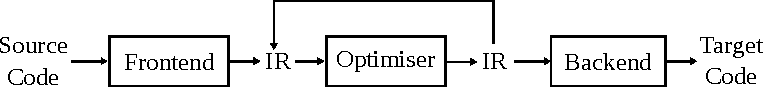
\includegraphics[scale=0.9]{figs/3-phase-compiler.pdf}
  \caption{Overview of the three-phase compiler infrastructure.}
  \label{fig:3-phase-compiler}
\end{figure}

%This IR is optionally fed through a series of analysis and optimization passes which improve the code, then is sent into a code generator to produce native machine code, as shown in Figure 11.3.
%This is a very straightforward implementation of the three-phase design, but this simple description glosses over some of the power and flexibility that the LLVM architecture derives from LLVM IR.

%The most important aspect of its design is the LLVM Intermediate Representation (IR), which is the form it uses to represent code in the compiler.
%LLVM IR is designed to host mid-level analyses and transformations that you find in the optimizer section of a compiler.
%It was designed with many specific goals in mind, including supporting lightweight runtime optimizations, interprocedural optimizations, whole program analysis, and aggressive restructuring transformations, etc.

%Like a real RISC instruction set, it supports linear sequences of simple instructions like add, subtract, compare, and branch.

\subsection{LLVM Virtual Instruction Set}

LLVM IR is a low-level RISC-like virtual instruction set.
It differs from other intermediate representations (e.g. GCC's GENERICS or the most recent GCC's GIMPLE) as it is defined as a first class language with well-defined semantics.
Beyond being implemented as a language, LLVM IR is actually defined in three isomorphic forms: the textual format above, an in-memory data structure inspected and modified by optimizations themselves, and an efficient and dense on-disk binary \textit{bitcode} format.
%The LLVM Project also provides tools to convert the on-disk format from text to binary: llvm-as assembles the textual .ll file into a .bc file containing the bitcode goop and llvm-dis turns a .bc file into a .ll file.

Unlike most RISC instruction sets, LLVM is strongly typed with a simple language-independent type system.
LLVM's type system can be used to implement data types and operations from high-level languages exposing their implementation behaviour to all stages of optimisation.
This type system includes the type information used by sophisticated techniques, such as algorithms for pointer analysis, dependence analysis, and data transformations.
LLVM also offers instructions for performing type conversions and low-level address arithmetic while preserving type information.
Furthermore, LLVM IR also differs from RISC instruction sets as some details of the machine are abstracted away.
For example, the calling convention is abstracted through call and ret instructions and explicit arguments.
Another significant difference from machine code is that the LLVM IR has an infinite set of virtual registers (which are named with a \% character), insted of having just a fixed set of named registers.

The LLVM type system is considered one of the most important features of its intermediate representation, as it enables several optimisations to be performed directly on the IR, without having to do extra analyses on the side before the transformation.
The main first class types supported are: single value types, aggregate types, and labels.
Single value types consist of integers of arbitrary bit width (e.g.\lstinline[language=llvm,style=nasm]{i32} denotes a 32-bit integer), floating-point of commonly used width (e.g.\lstinline[language=llvm,style=nasm]{half},\lstinline[language=llvm,style=nasm]{float},\lstinline[language=llvm,style=nasm]{double}, and\lstinline[language=llvm,style=nasm]{fp128}), pointers (e.g.\lstinline[language=llvm,style=nasm]{i32*}) and vector types.
Vectors are used when multiple primitive data are operated in parallel using a single instruction (SIMD).
A vector type is represented by a the number of elements and an underlying primitive data type, e.g.\lstinline[language=llvm,style=nasm]{<4 x i32>} is a vector of four 32-bit integer values.
Aggregated types consist of arrays and structures.
Vectors are not considered to be aggregate types.

In addition to type information, LLVM IR also provides other high-level information that are useful for effectively performing several code analysis and transformations.
This includes explicit control flow graphs (CFG)~\citep{allen70} and an explicit dataflow representation, by means of the infinite register set in \textit{static single assignment} form~\citep{alpern88,cytron89,cytron91}.

\subsubsection{Control Flow Graph}

A control flow graph (CFG) is a directed graph in which the nodes represent basic blocks and the edges represent control flow paths, i.e. edges represent transfers of control (jumps) between basic blocks.
A basic block is a straight-line sequence of instructions having only one entry point, i.e. the first instruction to be executed in the basic block, and only one exit point, i.e. the last instruction executed~\citep{allen70,cytron91}.
Figure~\ref{fig:cfg-odd_inc} shows an example of a CFG constructed from the code in Listing~\ref{lst:ex:odd_inc}.

\subsubsection{Static Single Assignment Form}

An IR is in \textit{static single assignment} (SSA) form if and only if each virtual register is assigned exactly once and every use of registers occur after their definition.
The primary advantage of using the SSA form is that it simultaneously simplifies and improves several compiler optimisations and analysis~\citep{alpern88,cytron91}.
Most of the industrial-strength compilers for imperative programming language rely heavily on the SSA form.

\begin{lstlisting}[language=llvm,style=nasm,caption={An illustrative example of a function in textual LLVM IR. This function returns the argument incremented by one if it is even or by two if it is an odd integer.}, label={lst:ex:odd_inc}]
define i32 @odd_inc(i32 %arg) {
entry:
  %rem = srem i32 %arg, 2
  %cmp = icmp eq i32 %rem, 0
  br i1 %cmp, label %if.then, label %if.else
if.then:
  %add.1 = add i32 %arg, 1
  br label %if.end
if.else:
  %add.2 = add i32 %arg, 2
  br label %if.end
if.end:
  %ans = phi i32 [ %add.1, %if.then ], [ %add.2, %if.else ] [!\label{lst:odd_inc:phi}!]
  ret i32 %ans
}
\end{lstlisting}

Listing~\ref{lst:ex:odd_inc} shows an example of a function written using textual LLVM IR.
Names starting with the @ character have a global scope, while names starting with \% have a local scope.
As stated previously, LLVM IR is strongly typed, which means that every virtual register is attributed a specific type (e.g.\lstinline[language=llvm,style=nasm]{i32 %arg} is of type\lstinline[language=llvm,style=nasm]{i32}, namely a 32-bit integer) as well as every operation (e.g.\lstinline[language=llvm,style=nasm]{add i32} expects all operands of type\lstinline[language=llvm,style=nasm]{i32}).
Instructions use the three address format, which refers to the use of three operands by most of the instructions.
However, instructions with fewer or more operands may occur, e.g. the\lstinline[language=llvm,style=nasm]{ret} instruction have fewer operands, while the\lstinline[language=llvm,style=nasm]{phi} and the\lstinline[language=llvm,style=nasm]{call} instructions may have more than three operands.

Furthermore, the SSA form requires a special assignment statements called the $\phi$-function (see line \ref{lst:odd_inc:phi} of Listing~\ref{lst:ex:odd_inc}).
The $\phi$-function receives as argument a list of virtual registers from different  control flow predecessors of the point where the $\phi$-function occurs.
The control flow predecessors of each point in the CFG are listed in some arbitrary fixed order, and the $i$-th operand of $\phi$-function is associated with the $i$-th predecessor.
If control reaches the $\phi$-function from its $i$-th predecessor, then the value of the $i$-th operand is attributed in the assignment.
Each execution of a $\phi$-function uses only one of the operands, but which one depends on the flow of control just before the $\phi$-function.

\begin{figure}[h]
  \centering
  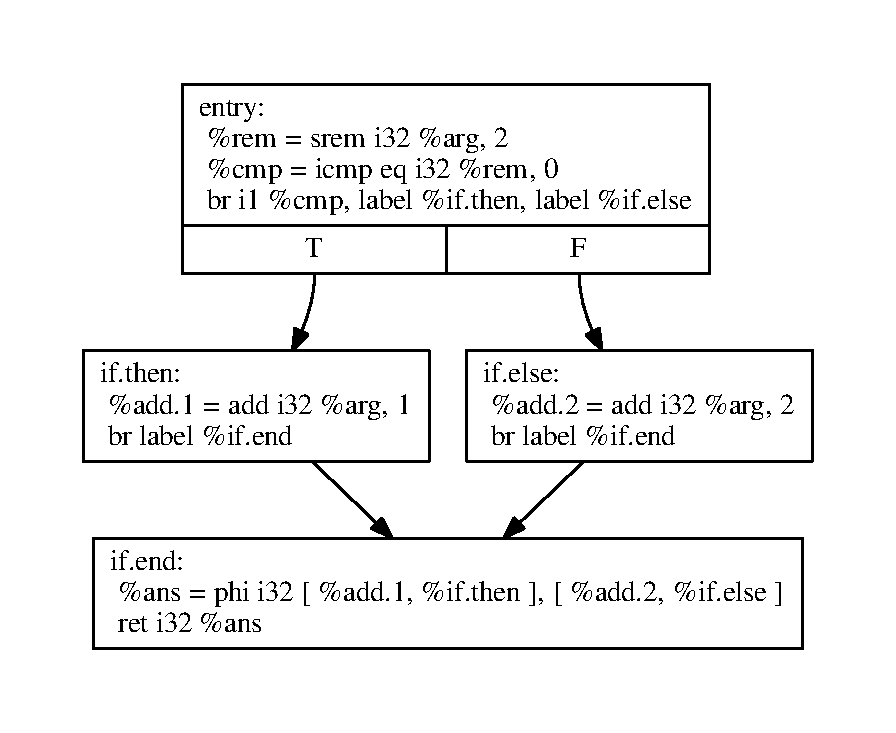
\includegraphics[scale=0.7]{figs/cfg-odd_inc.pdf}
  \caption{Control flow graph of the\lstinline[language=llvm,style=nasm]{odd_inc} function (see Listing~\ref{lst:ex:odd_inc}).}
  \label{fig:cfg-odd_inc}
\end{figure}

In addition to virtual registers, LLVM also allows for stack allocated local variables.
These are created by allocating data on the stack frame of the currently executing function.
Data from the stack frame can be manipulated by using explicit memory access operations.
Figure~\ref{lst:ex:odd_inc_stack} shows an implementation of the\lstinline[language=llvm,style=nasm]{odd_inc} function using data allocated on the stack frame.
This implementation avoids using the $\phi$-function by keeping the answer on the stack.
This is the preferred way of generating LLVM code by most frontends, as it simplifies the frontend's own implementation without incurring any serious detriment to the generated code.

LLVM provides an optimisation pass for promoting memory references to be register references (called \texttt{-mem2reg}).
It promotes alloca instructions which only have loads and stores as uses.
An alloca is transformed by using dominator frontiers to place phi nodes, then traversing the function in depth-first order to rewrite loads and stores as appropriate.

\begin{lstlisting}[language=llvm,style=nasm,caption={An example of the odd\_inc function implemented using data allocated on the stack frame.}, label={lst:ex:odd_inc_stack}]
define i32 @odd_inc_stack(i32 %arg) {
entry:
  %addr = alloca i32
  %rem = srem i32 %arg, 2
  %cmp = icmp eq i32 %rem, 0
  br i1 %cmp, label %if.then, label %if.else
if.then:
  %add.1 = add i32 %arg, 1
  store i32 %add.1, i32* %addr
  br label %if.end
if.else:
  %add.2 = add i32 %arg, 2
  store i32 %add.2, i32* %addr
  br label %if.end
if.end:
  %ans = load i32, i32* %addr
  ret i32 %ans
}
\end{lstlisting}

%\textbf{Another difference between LLVM and GCC:}

%In particular, LLVM IR is both well specified and the only interface to the optimizer.
%This property means that all you need to know to write a front end for LLVM is what LLVM IR is, how it works, and the invariants it expects.
%Since LLVM IR has a first-class textual form, it is both possible and reasonable to build a front end that outputs LLVM IR as text, then uses Unix pipes to send it through the optimizer sequence and code generator of your choice.

%It might be surprising, but this is actually a pretty novel property to LLVM and one of the major reasons for its success in a broad range of different applications.
%Even the widely successful and relatively well-architected GCC compiler does not have this property: its GIMPLE mid-level representation is not a self-contained representation.
%As a simple example, when the GCC code generator goes to emit DWARF debug information, it reaches back and walks the source level "tree" form.
%GIMPLE itself uses a "tuple" representation for the operations in the code, but (at least as of GCC 4.5) still represents operands as references back to the source level tree form.

%The implications of this are that front-end authors need to know and produce GCC's tree data structures as well as GIMPLE to write a GCC front end.
%The GCC back end has similar problems, so they also need to know bits and pieces of how the RTL back end works as well.
%Finally, GCC doesn't have a way to dump out "everything representing my code", or a way to read and write GIMPLE (and the related data structures that form the representation of the code) in text form. The result is that it is relatively hard to experiment with GCC, and therefore it has relatively few front ends.

\subsubsection{Dominators and Natural Loops}

A basic block $u$ dominates another basic block $v$ if and only if all paths 
to $v$ must also contain $u$.
In other words, any basic block that dominates all predecessors of $v$ also dominates $v$.

Natural loops are the cyclic structure in a CFG.
First we define a backedge, which is an edge $(u,v)$ such that $v$ dominates $u$.
Hence, a natural loop can be defined by the subgraph encompassed by its backedge.
That is, for any given backedge $(u,v)$, the subgraph consisting of all paths with origin $v$ and terminus $u$, in addition to the backedge itself, is a natural loop.

\begin{figure}[h]
  \centering
  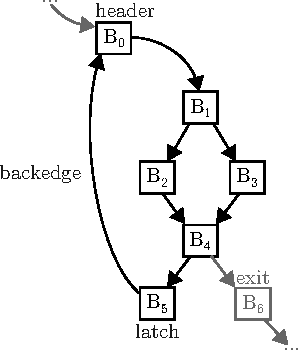
\includegraphics[scale=1]{figs/natural-loop.pdf}
  \caption{Example of natural loop.}
  \label{fig:natural-loops}
\end{figure}

Figure~\ref{fig:natural-loops} shows an example of a natural loop.
Natural loops contain a \textit{header} basic block, which is the entry basic block of the loop,
a \textit{latch} basic block, which is the origin of the backedge to the header of the loop.
It also contains one or more exit basic blocks, which are not part of the loop themselves but successors of basic blocks from the loop.
All basic blocks that comprise the natural loop can be found by a backwards \textit{depth-first search} that starts at the latch basic block and stops at the header.
 
\subsection{Analysis and Transformation Passes}

The LLVM optimiser offers several passes in order to provide analysis and transformation capabilities.
These passes are written using the LLVM Core libraries and they are as loosely coupled as possible.
In other words, each pass is either a stand-alone pass or it explicitly declares its dependencies among other passes, in the case where it depend on some other analysis.
A pass can also specify the analysis passes that will be invalidated by its execution.

The LLVM Core libraries provide both analysis and transformation passes for different levels of the input program.
These levels, in hierarchical order, are: module, call-graph SCC, function, loop, single-entry single-exit region (or only region for short), and basic block.
A module is an entire \textit{translation unit} (e.g., a C/C++ file with all its headers included).
A pass level only allows modification inside the component in focus.
For example: while a module-level pass can operate on the entire module at once,
a function-level pass prohibits any modification on the module-level (or other functions).

\begin{figure}[h]
  \centering
  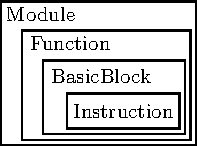
\includegraphics[scale=1]{figs/llvm-containers.pdf}
  \caption{The hierarchical levels in an LLVM input program. A call-graph SCC is a particular pattern amongst the functions in a module.
Similarly, a loop and a region are particular patterns on the CFG of a function.}
  \label{fig:llvm-containers}
\end{figure}

%\begin{description}
%\item[Module Pass:] This pass level allows the entire module to be analysed at once.
%\item[Function Pass:] This pass operates on each individual function contained in the module being processed.
%There is no particular order in which the functions will be considered.
%This pass level prohibits any modification on the module-level (or other functions).
%\item[Basic Block Pass:] This pass level considers one basic block at a time.
%\end{description}

The LLVM Pass Manager is responsible for scheduling the passes and make sure that the interactions among the passes are correctly fulfilled.
For that purpose, when given a series of passes to execute, the Pass Manager uses the explicit dependency information to satisfy these dependencies and optimise the execution of passes.
The Pass Manager aims at avoiding to repeat the execution of analysis passes.
It keeps track of which analyses are already available, which are invalidated, and which analyses are pending.
It also tracks the lifetimes of the analysis results and frees memory of the analysis results, when appropriate, managing memory usage.
%The Pass Manager pipelines the passes together to get a better memory and cache usage, improving the overall cache behaviour of the compiler.
For example, when performing a series of function-level passes, it executes all these passes in only one function, before moving to the next function, in order to improve the overall cache behaviour of the compiler.

Notice however, that the Pass Manager executes the transformation passes in the exact same order as they were requested, as changing this order may result in a different code.
Deciding on the best order to execute the transformation passes is a well known problem called the phase-ordering problem~\citep{touati06,kulkarni12,jantz14}.
The phase-odering problem is not addressed by the Pass Manager.

\section{{\IterComp} and its Space Exploration}

In this section we present the basic concepts of {\itercomp} and discuss some of the early work on this research topic.
We also consider some of the challenges on reducing its compilation time and present recent work that addresses these challenges.

{\Itercomp} is a well known compilation technique that searches the optimisation space in order to find the best optimisation for a particular program.
{\Itercomp} has the ability to adapt to new platforms, program and workload while still having a systematic and simple optimisation process.
It works by repeatedly evaluating a large number of compiler optimisations, by means of an execution-driven search, until the best optimisation is found for a particular program~\citep{kisuki99,fursin07,chen10}.
%The main challenge concerning {\itercomp} is the need for efficiently exploring such a large optimisation space~\citep{fursin07,cavazos07,zhou12}.

Figure~\ref{fig:itercomp-diagram} shows an overview of the architecture necessary for performing {\itercomp}.
After executing an optimised version of the program, profiling data is provided as a feed-back to the iterative search.
This profiling data can be as simple as the program's execution time, or more complex, including hardware performance counters for cache behaviour, measurements of energy consumption, etc.
The evaluator is able to use the feed-back in order to rank the optimisations and select the best one.
The optimisation generator can be a fixed sequence of optimisations or a dynamic mechanism for suggesting the next optimisation.

\begin{figure}[htb]
    \centering
    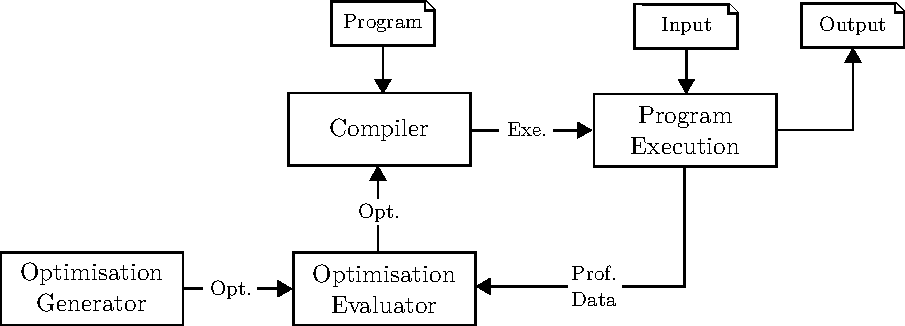
\includegraphics[width=\linewidth]{figs/itercomp-diagram}
    \caption{A simplified overview of the architecture of an iterative compiler.}
    \label{fig:itercomp-diagram}
\end{figure}

Early work on {\itercomp} have demonstrated its use for determining simultaneously optimal tile sizes and unroll factors for any given loop nest~\cite{kisuki00,knijnenburg04}.
These two transformations are highly interdependent with a very irregular optimisation space, as both of them affect, in different ways, cache behaviour and instruction-level parallelism.
Because of their close interaction, with non-trivial trade-offs, designing a static cost model, that enables the compiler to automatically select the best configuration, is a very laborious and impractical task.
\cite{kisuki00} propose the use of {\itercomp} to address this problem, where it is able to outperform several static techniques.
However, its success comes at the cost of a significant increase in compilation time, which involves several runs of the program for the execution-driven search.

Despite the high cost of compilation time, there are scenarios where this approach is highly attractive due to high-performance requirements, such as embedded systems and library codes.
Moreover, {\itercomp} was originally intended to be applied in an \textit{offline} scenario, where the software vendor optimises the program before shipping, the compilation time can be amortised across the number of products shipped, the lifetime of the product, or a much larger number of executions in production~\cite{kisuki99,kisuki00,chen10}.
It is also useful in contexts where the underlying architecture changes frequently, as the iterative search dismisses the arduous task of manually optimising the program for the new platform.

Numerous researchers have addressed the problem of reducing the optimisation space.
For the same problem of selecting optimal tile sizes and unroll factors, \cite{knijnenburg04} suggest the use of a cache model to avoid executing candidates during the execution-driven search of {\itercomp}.
By querying the cache model, the compiler is able to rank the optimisation candidates, filtering out candidates below a given threshold.
Their results show that it is possible to reduce the number of executions by up to about 70\%, without a significant degradation of the resulting optimisation.

\cite{agakov06} suggest using machine learning techniques to speed up {\itercomp}.
They propose a mechanism that learns a predictive model from a training set of benchmarks.
This predictive model will later be used for predicting regions of the optimisation space that are more likely to contain promissing results.
Their approach is able to significantly reduce the number of executions necessary for achieving good performance improvements with the iterative search.

More recently, \cite{ogilvie17} have proposed a strategy based on active learning techniques in order to focus the search on promissing optimisation candidates.
It avoids redundant candidates 
by using high-quality models which based on a combination of optimisation settings to predict the runtime of the training benchmarks.

The problem of reducing the optimisation space is out of the scope of this thesis.
Having a better search strategy would only improve our mechanism for online {\itercomp}.

%\section{Program Profiling}
%\textbf{Basic background about profiling in general}
%Progrma profiling concerns with the acquisition of dynamic information collected during the program's execution.
%Since early work, program profiling has been used mainly to find performance bottleneck and to focus optimisations.
%\cite{knuth71} introduces program profiling as a table of frequency counts that records execution frequency of each statement during a typical run of a program.
%This program profiling 
%\cite{knuth71} profiles the execution frequency of each FORTRAN statement during the execution of representative programs.
%Progrma profiling is particularly useful for providing 

\section{0-1 Knapsack Problem}

The \textit{0-1 knapsack problem} is a well known \textit{NP-hard} problem in combinatorial optimisation~\cite{martello00}.
For a given set of $n$ items, where each item has a profit $p_i$ and a weight $w_i$, the problem consists of selecting a sub-set of the items, such that the total weight of the sub-set does not exceed a pre-defined maximum capacity $c$ and whose total profit is a maximum.
Although the general knapsack problem allows to repeatedly \textit{pack} the same item, in the 0-1 knapsack problem each item can only be selected once, always considering the maximum capacity.
This problem is represented by the following integer linear programming model:
\begin{equation*}
\begin{aligned}
& \textrm{maximise }\quad \sum_{i=1}^{n} p_ix_i \\
& \textrm{subject to }\quad \sum_{i=1}^{n} w_ix_i \leq c
\end{aligned}
\end{equation*}
\[
x_i\in\{0,1\}, i\in\{1,\ldots,n\}
\]
where $x_i$ takes a value 1 if and only if item $i$ is packed.

Because it is an NP-hard problem, there is no algorithm with polynomial-time complexity on all cases.
The brute force algorithm evaluates all sub-sets of the items, resulting in a search over a full binary tree with complexity of $O(2^n)$.
However, this problem have been thoroughly studied and several exact algorithms for its solution have been proposed in the literature.
These exact algorithms are mainly based on two approaches, namely branch-and-bound or dynamic programming~\citep{martello77,martello99}.

The branch-and-bound approaches usually consist in computing an upper bound for each node of the tree.
This upper bound is then used to prune unpromising branches by comparing it to the current best solution.
A common strategy is to sort all items in decreasing order of ratio of profit per unit weight, whcih allows for efficiently computing upper bounds using a \textit{greedy} approach and also tends to maximise pruning opportunities~\citep{martello77,martello00}.

There are also many heuristics for efficiently selecting the sub-set of item while trying and maximise the total profit.
For example, a \textit{greedy} heuristic tries to maximise the total profit by sorting all items based on their profit-weight ratio and then eagerly selecting all items allowed by the maximum capacity as it iterates over the sorted items, in a single pass~\citep{dantzig57}.
This \textit{greedy} heuristic have a complexity of $O(n\log{n} + n)$, or just $O(n\log{n})$ for short.
Although heuristics are not guaranteed to find the best solution, they usually tend to efficiently find good or close to optimal solutions.

\section{Statistics}

Confidence Intervals ...

\subsection{Linear Regression}

In statistics, for a known dataset $\{y_i, x_{i,1}, x_{i,2}, \ldots, x_{i,k}\}_{i=1}^n$ of size $n$, a regression model creates a relation between the \textit{dependent variables} $y_i$ and the input variables $x_{i,j}$, also called \textit{regressors}, such that
\[
y_i \approx f(x_{i,1}, x_{i,2}, \ldots, x_{i,k})
\]

A well known regression model is the linear regression model, which assumes that there is a linear relation between regressors and the dependent variables.
In other words, it assumes that function $f$ has the form
\[
y_i = \varepsilon_i + \sum_{j=1}^k \beta_j x_{i,j}
\]
where $\beta_j$ are unknown parameters, also called \textit{regression coefficients},
and $\varepsilon_i$ are error terms.

%For a given dataset, the \textit{regression coefficients} and a single intercept term $\varepsilon$ can be estimated by a mathematical optimisation approach that tries to optimise for a given objective function. For example, it can minimise for the \textit{mean squared error}, i.e.,
%\[
%\min \quad MSE = \frac{1}{n} \sum_{i=1}^n\left(f(x_{i,1}, x_{i,2}, \ldots, x_{i,k}) - y_i\right)^2
%\]
%where $f$ is the linear function.

For a given dataset, the regression coefficients and an intercept term $\varepsilon$ can be estimated.
These estimated parameters can then be used to predict the dependent variable $y_i$ for new input variables $x_{i,j}$, not in the dataset.

There are many algorithms for parameter estimation, with different aspects and trade-offs~\citep{seber12}.
The linear regression model have been widely studied in the literature and describing specific algorithms for fitting the regression is out of the scope of this thesis.

\section{Summary}

\chapter{Related Work}

\section{{\IterComp}}

Until recently, most of existing work  had been focusing on finding the best optimisation through repeated runs using a single input.
Although they demonstrate the potential of {\itercomp}, in real scenarios the user rarely executes the same input dataset multiple times~\citep{bodin98,kisuki99,stephenson03,kulkarni04,agakov06}.
Applying {\itercomp} in light of a single input may not result in good performance when executing the optimised code with different inputs.

Most of real world applications are complex enough so that a single input case does not capture the whole range of possible scenarios and program behaviour~\citep{haneda06,fursin07,chen10,chen12a}.
Because programs can exhibit behaviours that differ greatly depending on the input, using a single input for {\itercomp} can produce poor performance when executed with different inputs.

For this reason, researchers have been studying the impact of using multiple input datasets for performing {\itercomp}.
\cite{chen10,chen12a} evaluate the effectiveness of iterative compilations across a large number of input test cases.
Their main motivation is to answer the question:
\textit{How data input dependent is {\itercomp}?}
When selecting the best optimisation sequence for each input of each program, these optimal optimisation sequences are program-specific and yield average speedups up to 3.75$\times$ over the highest optimisation level of compilers, namely {\flagstype -O3}.
Their results show that, for all the evaluated benchmarks, it is possible to find an optimisation sequence that achieves at least 83\% of the maximum speedup across all input test cases.
In other words, although the best optimisation sequences are both program and input-dependent, it is possible to find a program-specific optimisation sequence that achieves good performance on average.

When optimising a program, the main method for {\itercomp} used by \cite{chen10,chen12a} evaluates each combination of compiler optimisations across all the available inputs, i.e., if $N$ is the number of input test cases and $M$ is the total number of combinations of compiler optimisations, they perform a total of $O(NM)$ runs of the program being optimised.
Furthermore, they use a pre-defined set of only 300 different combinations of compiler optimisations, which represents a very small sample of the optimisation search space for most modern compilers, e.g.
LLVM has 56 distinct optimisation passes and GCC has about 47 high-level (SSA form) optimisation passes and about 25 low-level (RTL) optimisation passes, which in both cases result in much more than $2^{50}$ distinct combinations of compiler optimisations, without considering repetition.

Some recent work~\citep{chen12b,fang15} have applied the same idea of performing input-dependent {\itercomp} to distributed applications on data centres.
In summary, each worker receives a subset of the input dataset, called the evaluation dataset, to perform an \textit{online} {\itercomp} of the code being executed.
Each worker performs the same the method for {\itercomp} used by \cite{chen10,chen12a}, i.e., they evaluate each combination of compiler optimisations across all the evaluation dataset.
However, because the optimisation is performed online, they usually consider a small evaluation dataset and a small number of compiler optimisations.

\cite{fursin07} addressed the problem of comparing the effect of two optimisations on two distinct inputs.
For that purpose, they proposed to use instructions per cycle (IPC) as the metric for performing such comparison.
Their result show that using IPC seems promising as a robust metric for {\itercomp} across large input datasets.
However, some specific optimisation techniques may affect the use of IPC as a robust metric, and specially IPC has been shown to provide poor performance estimation for multi-threaded programs~\citep{alameldeen06,eyerman08}.
In particular, IPC can give a skewed performance measure if threads spend time in \textit{spin-lock loops} or other synchronisation mechanisms. 
Some existing work on performance assessment suggest that total execution time should be used for measuring performance of multi-threaded programs~\citep{alameldeen06,eyerman08}.
\cite{alameldeen06} in particular suggest that a simple work-related metric should be used if the unit of work is representative enough.
Work-related metrics have already been largely used for measuring performance of throughput-oriented applications, for other applications, however, choosing an appropriate unit of work can be more challenging~\citep{alameldeen06}.

\section{Work and Input Size Metrics}

\textbf{Talk about work-based metrics}

\citep{mcgeoch07}

Previous work have proposed profiling-based mechanism to estimate input sizes~\citep{zaparanuks12,coppa14}.
\cite{coppa14} in particular propose the concept of \textit{read memory size} for automatically estimating the size of the input passed to a routine, where \textit{read memory size} represents the number of distinct memory cells first accessed by a read operation.
In other words, the \textit{read memory size} metric measures the size of the useful portion of the input's memory footprint.
However, because we are interested in the amount of computational work performed in respect of a given input, the memory footprint of the input may not always have a direct correspondence to  the amount of computational work.

\cite{goldsmith07} use \textit{block frequency} as the measure for performance for empirically describing the asymptotic behaviour of programs, which is known as empirical computational complexity.
Block frequency is a relative metric that represents the number of times a basic block executes~\citep{ball94,ball96}.
They argue in favour of block frequency due to its portability, repeatability and exactness, since it does not suffer from timer resolution problems or non-deterministic noises.
Block frequency also has the advantage of being efficiently profiled by means of automatic code instrumentation~\citep{knuth73,ball94}.

However, in the context of comparing different optimisations, although block frequency would be able to capture aspects of optimisations that simplify the control-flow graph (CFG), measuring work at the basic block resolution would not capture effects of optimisations at the instruction level.
Because of that, we extend the idea of using basic block frequency to measure computational work by also considering the computational cost of each basic block.
The computational cost of a basic block is given by weighting the instructions that it contains.

\section{Progrma Profiling} \label{subsec:optimalInstrumentation}

\textbf{TODO: }
Progrma profiling concerns with the acquisition of dynamic information collected during the program's execution.
Since early work, program profiling has been used mainly to find performance bottleneck and to focus optimisations.
\cite{knuth71} introduces program profiling as a table of frequency counts that records execution frequency of each statement during a typical run of a program.
This program profiling 
\cite{knuth71} profiles the execution frequency of each FORTRAN statement during the execution of representative programs.


In order to profile  block frequency, the program can be instrumented with counters that determine how many times each basic block in a program executes.
A naive instrumentation would consist basically of having a counter for each basic block which is incremented every time the basic block is reached.
Although the naive instrumentation was commonly used in practice~\citep{knuth71}, it is a very invasive instrumentation that imposes an unnecessarily high overhead in the instrumented program.
An optimal instrumentation based on the principle of \textit{conservation of flow} (\textit{Kirchhoff's first law}\footnote{Gustav Kirchhoff defined two equalities about electric circuits, known as Kirchhoff's circuit laws. The first one is about current and and the second about potential difference.}) have been originally proposed by \cite{nahapetian73} and \cite{knuth73}.
While \cite{knuth73} proposed an optimal solution for basic block profiling with \textit{vertex counters}, \cite{ball94} showed that an optimal basic block profiling with \textit{edge counters} provides the best instrumentation for block-frequency profiling.
Further overhead reduction of the optimal instrumentation was later proposed by placing the counters in edges that are less likely to be executed~\cite{forman81,ball94}.

\begin{definition}[Kirchhoff's first law]
The amount of flow into a vertex equals the amount of output flow, i.e. the sum of the incoming edges of a vertex equals the sum of outgoing edges of the same vertex.
\end{definition}

The optimal instrumentation places probes in edges as the basic block frequency can be derived by summing either the flow of the incoming or outgoing edges.
However, it uses the Kirchhoff's first law in order to place probes in subset of the edges that allows to later infer the flow of all edges.
Previous work have shown that a set of edges represents the minimum number of probes for profiling block frequency if and only if the complementary set of edges forms a spanning tree~\citep{nahapetian73,ball94}.
In other words, after determining a spanning tree of the CFG, probes need to be placed only in the edges from the complement of a spanning tree, usually called \textit{cotree}.
Because the edge frequencies satisfy Kirchhoff's first law, each edge flow can be uniquely determined as an algebraic sum of the known edge flows from the cotree~\citep{nahapetian73,ball94}.

The optimal block-frequency instrumentation happens in two main stages:
\textit{(i.) Before execution.} The code is instrumented with the edge counters, i.e., it requires one global counter for each edge selected to contain a probe.
\textit{(ii.) After execution.} The information from the recorded probes is propagated in the CFGs of the program.
\lstlistingname~\ref{lst:populateEdgeFlows} shows the algorithm for the post-processing of a CFG, which requires the profiling information collected by the probes.

\begin{lstlisting}[caption={Post-processing of the CFG for populating all edge flows based on the collected probes.}, label={lst:populateEdgeFlows}, float]
// Inputs: CFG with the known edges flows from the cotree (collected probes).
// Output: Updated CFG with all edge flows.
populateEdgeFlows(G) {
  changed = true
  while changed:
    changed = false
    for B in G.vertices():
      unIN = count( G.unknownIncomingEdges(B) )
      unOUT = count( G.unknownOutgoingEdges(B) )
      if unIN==0 and unOUT==1:
        //sum known incoming and outgoing edges in B
        sIN = sum( G.incomingEdges(B) )
        sOUT = sum( G.outgoingEdges(B) )
        //update unknown outgoing edge in B with (sIN-sOUT)
        G.setUnknownOutgoingEdge(B, (sIN-sOUT))
        changed = true
      if unIN==1 and unOUT==0:
        //sum known incoming and outgoing edges in B
        sIN = sum( G.incomingEdges(B) )
        sOUT = sum( G.outgoingEdges(B) )
        //update unknown incoming edge in B with (sOUT-sIN)
        G.setUnknownIncomingEdge(B, (sOUT-sIN))
        changed = true
}
\end{lstlisting}

\lstlistingname~\ref{lst:populateEdgeFlows} is guaranteed to terminate because the probed edge flows on the complement of a spanning tree are necessary and sufficient to compute all edge flows~\citep{nahapetian73,forman81}.
Intuitively, if all the edge flows are known for the complement of a spanning tree then at any leaf of the spanning tree there is only one unknown edge flow.
This unknown edge flow can be calculated by Kirchhoff's first law.
This process repeats until all the unknown edge flows have been calculated.
Although this instrumentation algorithm is proved to produce the optimal placement of probes for well-structured CFGs, it may produce sub-optimal placement for some unstructured CFGs~\citep{ball94}.

This briefly described proof suggests that the edges can be more efficiently populated by a bottom-up propagation in the spanning tree.
By performing a post-order traversal of the spanning tree, i.e. starting from the leaves, we can then apply the flow equation from the Kirchhoff's first law.
At each node of the spanning tree, we first sum the known incoming and outgoing edges, and then the unknown edge flow will by computed by subtracting the minimum of the two sums from the maximum (as before).
This bottom-up propagation allows to populate the edge flows in a single pass over the basic blocks.

\cite{forman81} and \cite{ball94} propose to optimise the placement of the probes with respect to edges that are less likely to be executed.
It works by considering a weighting that assigns a non-negative value to each edge in the CFG.
The overhead cost of profiling a set of edges is considered to be proportional to the sum of the weights of the edges.
These weights can be obtained either by empirical measurements from previous executions or by static estimates at compile-time.
In order to minimise the profiling overhead, the instrumentation computes the maximum spanning tree in order to avoid probing in frequently executed edges.

\lstlistingname~\ref{lst:instrumentCFG} presents the algorithm for the optimal placement of probes.
If present, it uses edge-frequency profiling from previous executions,
otherwise it uses static estimates of edge frequencies.
Afterwards, it makes use of the edge frequencies for computing the maximum spanning tree.
LLVM implements Kruskal's algorithm using the union-find data structure~(see \lstlistingname~\ref{lst:kruskalMST})
for computing the maximum spanning tree of the CFG.
Only edges in the cotree are instrumented.

\begin{lstlisting}[caption={Optimal placement of probes for block frequency.}, label={lst:instrumentCFG}]
// Input: CFG	
instrumentCFG(G) {
  if not hasEdgeFrequency(G):
    estimateEdgeFrequency(G)
  T = MaxSpanningTree(G)
  for e in G.edges()-T.edges():
    placeProbe(e)
}
\end{lstlisting}

Because edges in a CFG are abstractions for a transition of control flow,
the actual code for the probes need to be placed in one of the endpoints of instrumented edges.
\lstlistingname~\ref{lst:placeProbe} selects which basic block of an edge will be instrumented.
\textit{Critical edges} are split, inserting a new basic block between its endpoints.
Critical edges are edges from a basic block that contains multiple successors to a basic block that contains multiple predecessors.

\begin{lstlisting}[caption={For a given edge, this procedure selects which basic block to place the instrumented code.
                            If the edge is critical, an intermediate basic block is created for the instrumentation.}, label={lst:placeProbe}]
// Input: edge selected for instrumentation
placeProbe(e){
  (B1, B2) = e
  if B1 is virtual:
    insertProbe(B2)
  else if B2 is virtual:
    insertProbe(B1)
  else if countSuccessors(B1)<=1:
    insertProbe(B1)
  else if e is not critical:
    insertProbe(B2)
  else
    B = splitCriticalEdge(e)
    insertProbe(B)
}
\end{lstlisting}

Notice that when instrumentation is performed guided by empirical measurements from previous executions, it means that edge-profiling information is used in order to produce a better edge-profiling instrumentation.
The next section presents the main algorithms for producing static estimates for the weights of the edges in a CFG.

\subsection{Static Estimates of Edge Frequencies}

\cite{ball93} presented a simple algorithm that predicts the outcome of conditional branches with a reasonably good accuracy.
For this purpose, they used several branch heuristics that were derived by measuring, on a large number of programs, the probability of branches being taken in respect of some \textit{ad-hoc} features from the programs.
Their algorithm selects, for each branch, the first heuristic that applies to the branch, in a given priority order of the heuristics.
The \textit{ad-hoc} heuristics defined by \cite{ball93} are:

\noindent\textbf{Loop branch heuristic (probability 88\%):} Probability of an edge back to a loop's head being executed.

\noindent\textbf{Loop exit heuristic (probability 80\%):} Probability that a comparison inside a loop will \textit{not} exit the loop. This heuristic does not apply to latch blocks, i.e. basic blocks that contain a branch back to the header of the loop.

\noindent\textbf{Pointer heuristic (probability 60\%):} Probability that a comparison between two pointers, where one of them can be a null pointer, will fail.

\noindent\textbf{Opcode heuristic (probability 84\%):} Probability that a comparison of an integer being less than zero, less than or equal to zero, or equal to a constant will fail.

\noindent\textbf{Guard heuristic (probability 62\%):} For a comparison with a register as operand, where the register is defined in a successor basic block which is not a post-dominator. The probability that the successor basic block is reached.

\noindent\textbf{Loop header heuristic (probability 75\%):} Probability of reaching a successor block that is a loop header (or pre-header) but not a post-dominator.

\noindent\textbf{Call heuristic (probability 78\%):} Probability of reaching a successor block that is not a post-dominator but contains a function call.

\noindent\textbf{Store heuristic (probability 55\%):} Probability of reaching a successor block that is not a post-dominator but contains a store instruction.

\noindent\textbf{Return heuristic (probability 72\%):} Probability of reaching a successor block that contains a return instruction.


\cite{wu94} proposed an algorithm for statically estimating edge frequencies, which improves on the work of \cite{wagner94} and \cite{ball93}.
This algorithm is able to combine several heuristics of the outcome of a branch into an estimated probability of the branch being taken.
\cite{wu94} use the \textit{ad-hoc} heuristics defined by \cite{ball93} as their initial predictions.
They also use the Dempster-Shafer theory~\citep{shafer76} that provides the necessary mathematical technique for combining evidences from the different heuristics in order to produce more accurate estimates.
These branch probabilities can then be used to estimate execution frequencies
for all the edges in a CFG.

\section{Summary}

%
\chapter{Work-based Metric} \label{sec:metric}

In this section we define the work-based performance metric proposed for comparing different optimised versions of a program when executing with different inputs.
We define the performance metric as the ratio between the amount of \textit{work}, $\Delta W$, performed during a period of time, $\Delta t$.
\[
   P = \frac{\Delta W}{\Delta t}
\]

%The hypothesis is that, given two optimisations $o_1$ and $o_2$, a program compiled with optimisation $o_2$ would \textit{consistently} perform better than when it is compiled with $o_1$, i.e., $o_1 \tilde{<}_p \, o_2$, if it performs more \textit{work} per unit of time when compiled with $o_2$ instead of $o_1$. 
By measuring the amount of \textit{work} done per unit of time we reduce the impact of input-dependent aspects and focus instead on the efficiency of the optimised program.
For this metric, the main challenge is to precisely define what represents \textit{work}.

%For that purpose, we intend to use profiling techniques to measure the input size and amount of computation performed on the execution path triggered by the input~\cite{ball94,ball96,zaparanuks12,coppa14}.

%In addition to being useful for speeding up {\itercomp} across a large number of different inputs, this metric based on comparing work-based efficiencies could
%potentially be used for applying {\itercomp} \textit{online}.
%However, the overhead for estimating the amount of \textit{work} must be low enough for the performance gains to be beneficial.

We model the computational work $\Delta W$ as a linear equation based on block frequency information and a cost-model of the instruction set.
\[
\Delta W = \varepsilon + \sum_{B} w(B)f(B)
\]
where $f(B)$ represents the frequency of basic block $B$ and $w(B)$ represents the computational work of executing $B$.
We define the work of a basic block $B$ as the sum of the cost of its instructions, i.e.,
\[
w(B) = \sum_{i} w_i N_B(i)
\]
where $w_i$ is the cost of instruction $i$ and $N_B(i)$ is the number of occurrences of instruction $i$ in basic block $B$.

In this simplified model, we consider that $w_i$ is constant across all programs and executions in the given target platform.
However, $N_B(i)$ is program dependent but constant across executions, while $f(B)$ is both program and execution dependent, since $f(B)$ can change when executing with different inputs.
In other words, $N_B(i)$ is a static value known at compile-time and $f(B)$ is a dynamic value known only at run-time.
%If we define $x_i$ as
%\[
%x_i = \sum_{B\in P} N_B(i)f(B)
%\]
%we can write our definition of work $\Delta W$ as the following linear equation
%\[
%\Delta W = \varepsilon + \sum_{i\in I} w_i x_i
%\]

%\subsection{Linear regression}
%
%\begin{figure}[htb]
%    \centering
%    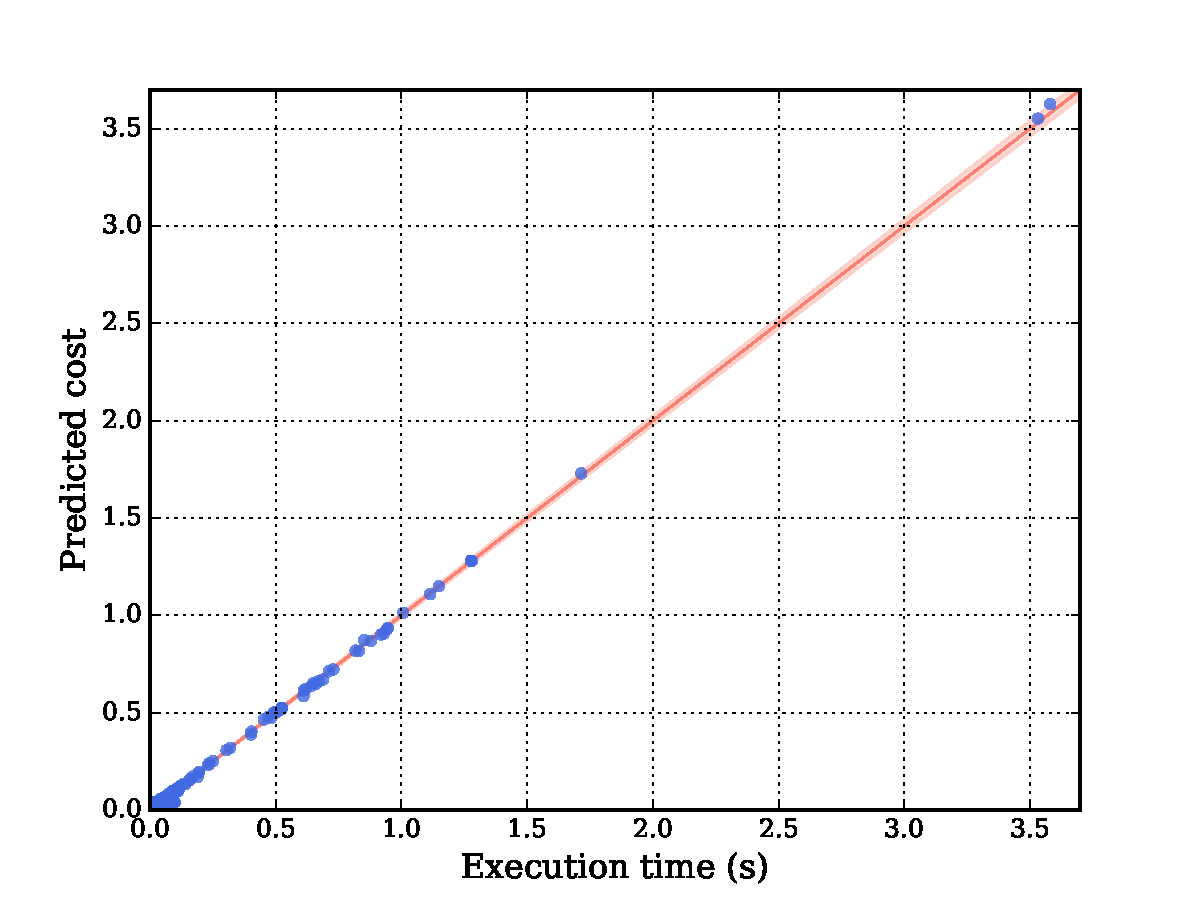
\includegraphics[width=\linewidth]{figs/cost-model.pdf}
%    \caption{Comparison between the naive and optimal instrumentation with no compiler optimisation.} %, i.e., compiled with \textbf{\texttt{-O0}}.}
%    \label{fig:cost-model}
%\end{figure}
%mse 0.000145373168444
%mae 0.00737261168981
%mae* 0.0033892281406
%mape 75.2924320971
%corr (0.99946441743545622, 0.0)

Similarly to previous work~\citep{giusto01,powell09,brandolese11}, we derive the cost model for the instruction set by modelling the problem as a multi-variable linear regression, where the \textit{regression coefficients} are the costs of the instructions and the \textit{regressors} (or \textit{explanatory variables}) are computed as $\sum_B N_B(i)f(B)$ for each instruction $i$.
\[
\Delta W = \varepsilon + \sum_{i} \left(w_i \sum_{B} N_B(i)f(B)\right)
\]

By having some empirical data after executing several benchmarks with different inputs, we can fit the linear model with this empirical data in order to obtain the costs of the instructions.

\begin{figure}[htb]
    \centering
    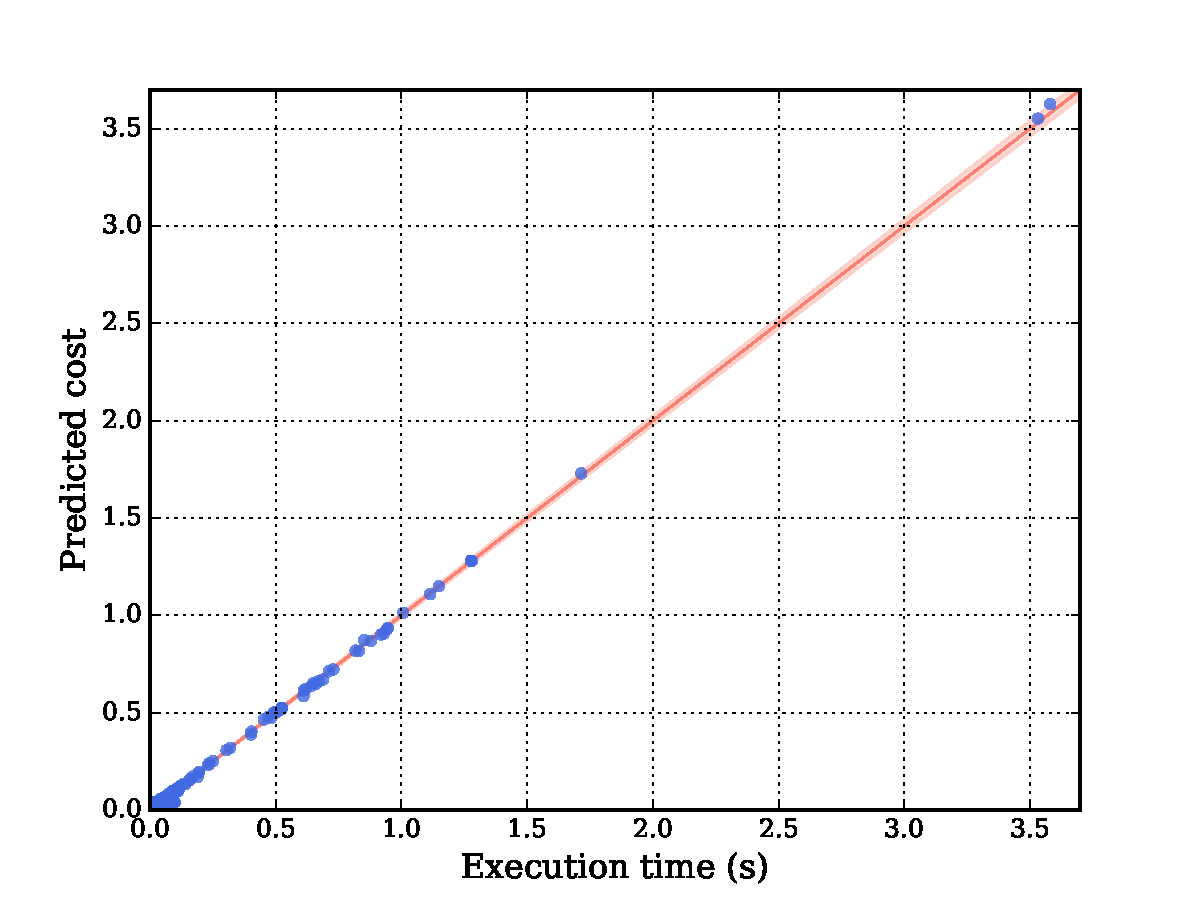
\includegraphics[width=0.9\linewidth]{figs/cost-model.pdf}
    \caption{Linear model fitted from empirical data. The mean absolute error (MAE) for the fitted curve is of 7 milliseconds.}
    \label{fig:cost-model}
\end{figure}


\chapter{Online {\IterComp}}

\section{Work-based Metric}\label{sec:metric}

In this section we define the work-based performance metric proposed for comparing different optimised versions of a program when executing with different inputs.
We define the performance metric as the ratio between the amount of \textit{work}, $\Delta W$, performed during a period of time, $\Delta t$.
\[
   P = \frac{\Delta W}{\Delta t}
\]

%The hypothesis is that, given two optimisations $o_1$ and $o_2$, a program compiled with optimisation $o_2$ would \textit{consistently} perform better than when it is compiled with $o_1$, i.e., $o_1 \tilde{<}_p \, o_2$, if it performs more \textit{work} per unit of time when compiled with $o_2$ instead of $o_1$. 
By measuring the amount of \textit{work} done per unit of time we reduce the impact of input-dependent aspects and focus instead on the efficiency of the optimised program.
For this metric, the main challenge is to precisely define what represents \textit{work}.

%For that purpose, we intend to use profiling techniques to measure the input size and amount of computation performed on the execution path triggered by the input~\cite{ball94,ball96,zaparanuks12,coppa14}.

%In addition to being useful for speeding up {\itercomp} across a large number of different inputs, this metric based on comparing work-based efficiencies could
%potentially be used for applying {\itercomp} \textit{online}.
%However, the overhead for estimating the amount of \textit{work} must be low enough for the performance gains to be beneficial.

We model the computational work $\Delta W$ as a linear equation based on block frequency information and a cost-model of the instruction set.
\[
\Delta W = \varepsilon + \sum_{B} w(B)f(B)
\]
where $f(B)$ represents the frequency of basic block $B$ and $w(B)$ represents the computational work of executing $B$.
We define the work of a basic block $B$ as the sum of the cost of its instructions, i.e.,
\[
w(B) = \sum_{i} w_i N_B(i)
\]
where $w_i$ is the cost of instruction $i$ and $N_B(i)$ is the number of occurrences of instruction $i$ in basic block $B$.

In this simplified model, we consider that $w_i$ is constant across all programs and executions in the given target platform.
However, $N_B(i)$ is program dependent but constant across executions, while $f(B)$ is both program and execution dependent, since $f(B)$ can change when executing with different inputs.
In other words, $N_B(i)$ is a static value known at compile-time and $f(B)$ is a dynamic value known only at run-time.
%If we define $x_i$ as
%\[
%x_i = \sum_{B\in P} N_B(i)f(B)
%\]
%we can write our definition of work $\Delta W$ as the following linear equation
%\[
%\Delta W = \varepsilon + \sum_{i\in I} w_i x_i
%\]

%\subsection{Linear regression}
%
%\begin{figure}[htb]
%    \centering
%    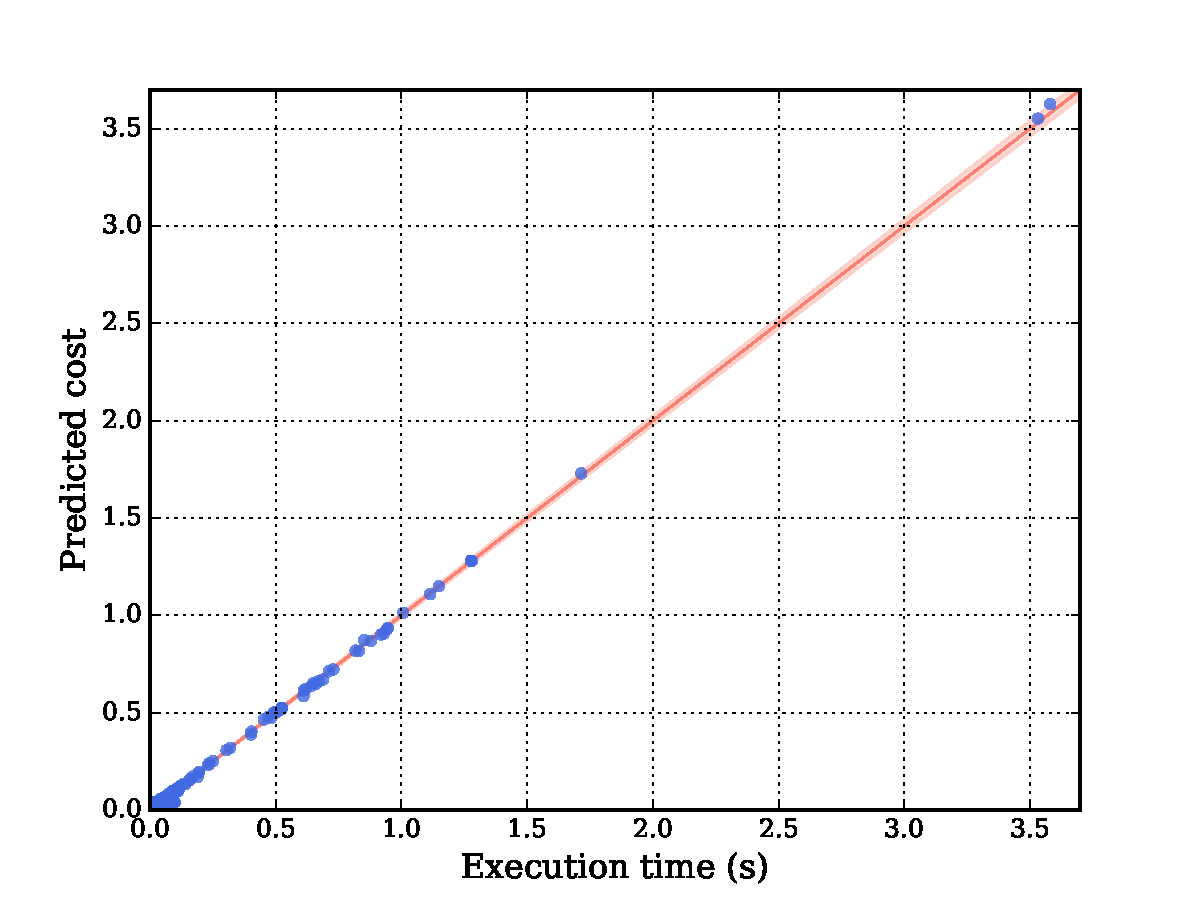
\includegraphics[width=\linewidth]{figs/cost-model.pdf}
%    \caption{Comparison between the naive and optimal instrumentation with no compiler optimisation.} %, i.e., compiled with \textbf{\texttt{-O0}}.}
%    \label{fig:cost-model}
%\end{figure}
%mse 0.000145373168444
%mae 0.00737261168981
%mae* 0.0033892281406
%mape 75.2924320971
%corr (0.99946441743545622, 0.0)


\subsection{Estimating a Cost Model of the Instructions}

Similarly to previous work~\citep{giusto01,powell09,brandolese11}, we derive the cost model of the instruction set by modelling the problem as a multi-variable linear regression, where the \textit{regression coefficients} are the costs of the instructions and the \textit{regressors} (or \textit{explanatory variables}) are computed as $\sum_B N_B(i)f(B)$ for each instruction $i$.
\[
\Delta W = \varepsilon + \sum_{i} \left(w_i \sum_{B} N_B(i)f(B)\right)
\]

By having some empirical data after executing several benchmarks with different inputs, we can fit the linear model with this empirical data in order to obtain the costs of the instructions.
In order to fit the linear model, we measure the wall-clock time when executing the training benchmarks described in Section\ref{} with their respective 1000 input datasets.
For these measurements, the training benchmarks are compiled without optimisation.
The reason for using no optimisation is because it allows to use the trained cost model for computing a work metric which is independent of optimisations, as we explained in Section~\ref{}.

\begin{figure}[htb]
    \centering
    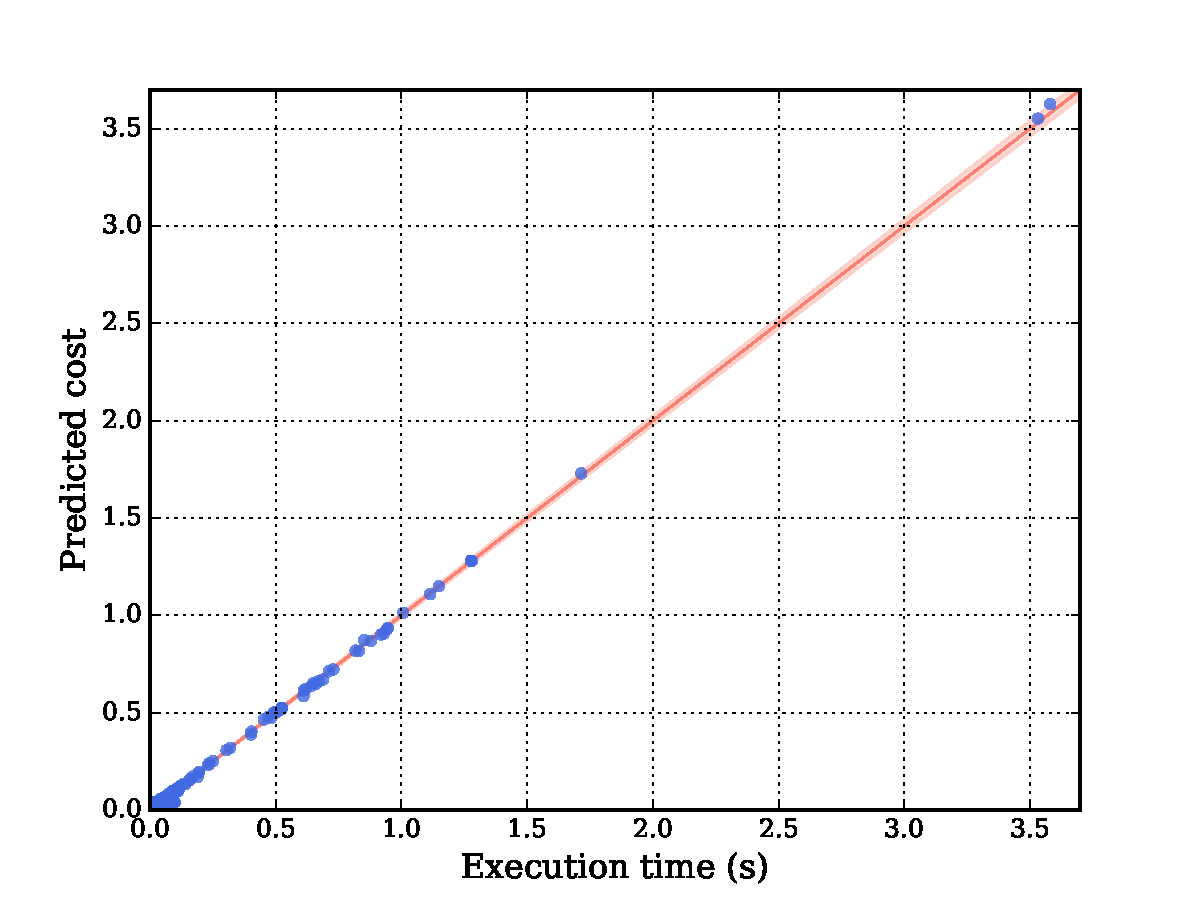
\includegraphics[width=0.9\linewidth]{figs/cost-model.pdf}
    \caption{Linear model fitted from empirical data. The mean absolute error (MAE) for the fitted curve is of 7 milliseconds.}
    \label{fig:cost-model}
\end{figure}

Because we fit the linear model based on the wall-clock execution time, the derived cost model can be interpreted as an estimate of the execution time when the program is compiled without optimisations.
Figure~\ref{fig:cost-model} compare the work metric with the corresponding execution time for some instances of the test benchmarks.
Notice how the fitted model has a higher relative error for the instances with very short execution time, namely those that run for less than one tenth of a second.
The mean absolute error (MAE) for the fitted curve is of 7 milliseconds.

\subsection{Comparison with Instructions Per Cycle} \label{sec:ipc-vs-work-metric}

The IPC metric have been widely used for studying performance benefits of hardware optimisations.

The proposed work-based performance metric differs from IPC in a key aspect:
the IPC metric is computed soley on the final optimised program.
For different optimisations of the same program, both the number of instructions and the number of cycles can change for the same input.
On the other hand, the work-based performance metric computes the amount of work based on the unoptimised program, which means that it always consider the same amount of work for the same input, regardless of the optimisations applied on the program.

For this reason, higher IPC does not necessarily translates to shorter execution time.
We can illustrate this fact with an example as shown in Table~\ref{}.
Although program P1 has twice the IPC of P2, P1 is one cycle slower than P2.
As this example illustrates, the IPC metric can be misleading when compared different versions of the same program.

\begin{table}[h]
\centering
\begin{tabular}{|c|c|c|c|}
\hline
                       & P1 & P2  \\
\hline
Number of Instructions & 5  & 2   \\
Number of Cycles       & 5  & 4   \\
IPC                    & 1  & 0.5 \\
\hline
\end{tabular}
\caption{Example that illustrates that a higher IPC does not necessarily translates to shorter execution time.}
\label{tab:ipc-example}
\end{table}

\section{Online {\IterComp} Infrastructure} \label{sec:oic-infra}

Although {\itercomp} had been originally proposed as an \textit{offline} optimisation strategy it can also be adapted to work in the online scenario.
Instead of selecting the best optimisation sequence as part of the development time (pre-shiping) of a program, a first version of the program is shipped together with a {\itercomp} mechanism.
In the online scenario, the program is shipped with a initial optimisation sequence and different optimisation sequences are evaluated as the end-user executes the program.
This optimisation strategy is also known as idle-time optimisation, as the re-compilation happens between runs of the program.

LLVM is particularly suitable for iterative compilation as it makes possible to cache a pre-compiled, but still unoptimised, version of the input program in the bitcode format of the LLVM IR.  
This caching allows to speedup the time required for re-compilation as it is able to bypass the frontend phase.
If re-compilation time is critical, it would also be possible to keep only the hot portion of the code in the LLVM bitcode format, while the remaining portion of the code is already in the format of object code.
However, this is out of the scope of this work and we always re-compile the whole program.

\begin{figure}[htb]
    \centering
    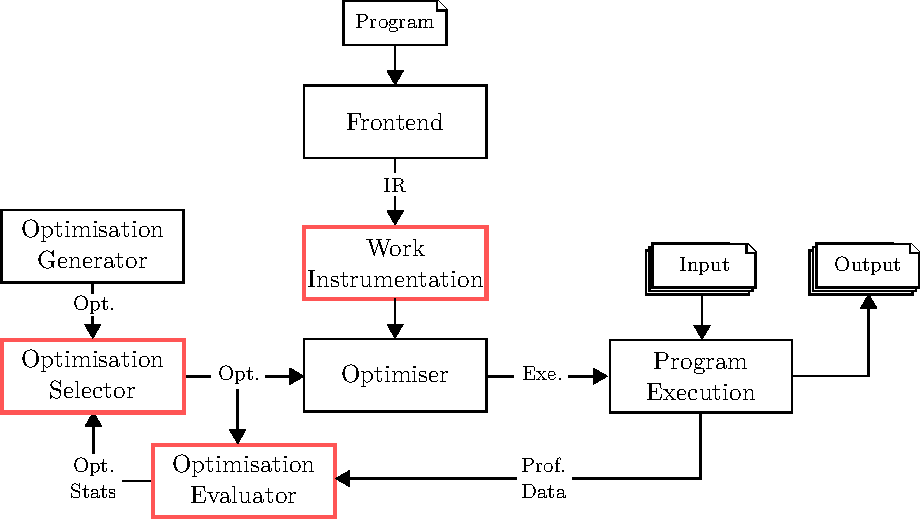
\includegraphics[width=\linewidth]{figs/infra-diagram}
    \caption{Overview of the execution engine for applying {\itercomp}.}
    \label{fig:infra-diagram}
\end{figure}
%\textbf{Describe the process step by step.}

Figure~\ref{fig:infra-diagram} shows an overview of the infrastructure required for applying online {\itercomp},
using the work-based performance metric as the metric of choice for evaluating optimisation sequences.
The online {\itercomp} follows as described bellow:
\begin{enumerate}
\item The program is pre-compiled to the LLVM bitcode format without optimisation.
\item The unoptimised program is instrumented for work profiling.
\item Execution-based optimisation seach:
 \begin{enumerate}
   \item The current optimisation sequence is used for the re-compilation of the program.
   \item The program is executed with any input provided by the end-user.
         During the execution of the program, wall-clock time and the work metric are recorded by profiling instrumentation.
   \item If the recorded profiling for the current optimisation can be used to compute an average performance measurement within a small confidence interval,
         then a new optimisation sequence is generated.
         Otherwise, the same optimisation sequence is used for the next execution.
 \end{enumerate}
\end{enumerate}

In this work we focus mainly on the two highlighted components.
In both phases the goal is to improve the performance of the execution phase, but from different perspectives.
\textit{(i.)} In the compilation phase we focused on providing a low-overhead instrumentation for profiling the work metric. This phase is responsible to improve performance by lowering the overhead of the work profiling.
\textit{(ii.)} In the evaluation phase we proposed the use of the work-based metric in order to enable {\itercomp} in an online scenario. This phase is responsible to improve performance by being able to properly assess different optimisations such that the best optimisation can be selected.
Chapter~\ref{chap:instr} describes our work profiling strategy and Section~\ref{sec:metric} describes the work-based metric.

%\textbf{Talk about the process of keeping the same optimization for a given input-window and how the optimizations as selected based on the evaluation of these "evidences". Perhaps we could suggest using the Theory of Evidences at this point?!}

In most online scenarios, it is common for periods of peak usage and idle periods.
For example, mobile devices are usually intensely used during the day, with some idle periods at night while its battery is being re-charged.
The proposed infrastructure is very well suited for these online scenarios as multiple runs of the program can be monitored during peak time, by collecting the work profiling and measuring its execution time, while at the idle time, the profiling statistics can be used for selecting better optimisations and re-compiling the program.
However, if idle time is almost non-existent, the proposed infrastructure can still be used by re-compiling the program with a different optimisation while multiple runs of the program are being executed.


\chapter{Work Instrumentation} \label{chap:instr}

In this section we describe how the computation of the work-metric can be performed during runtime by means of instrumenting the code.
In particular, we adapt the optimal algorithm proposed originally for block-frequency profiling~\citep{nahapetian73,knuth73,ball94}.
Afterwards, we propose a relaxed instrumentation that focus on further reducing the overhead by considering the trade-off between profiling accuracy and instrumentation overhead.

Because we define work as a linear equation on the block-frequency counters, it is possible to embed its computation into the execution of the program.
A naive instrumentation would consist basically of having a global counter that starts with the interception value, $\varepsilon$, and each basic block increments its own cost into the global counter.
Although this instrumentation is easily implemented, it imposes a large overhead on the instrumented program.
However, it is possible to insert fewer probes by carefully placing the probes in a way that is possible to reconstruct the complete profiling information~\cite{knuth73,ball94}.

\begin{figure}[h]
  \centering
  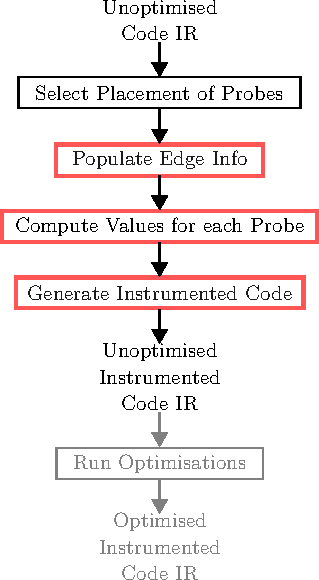
\includegraphics[scale=0.9]{figs/instr-diagram.pdf}
  \caption{Overview of the work instrumentation algorithm.}
  \label{fig:instr-diagram}
\end{figure}

We adapt the optimal block-frequency instrumentation in order to perform the work profiling efficiently.
The proposed work instrumentation differs from the optimal block-frequency instrumentation as the latter occurs in two stages:
\textit{(i.) Before execution.} The code is instrumented with counters for each probe.
\textit{(ii.) After execution.} The information from the recorded probes is propagated in the CFGs of the program.
In contrast, the work instrumentation has a single counter and it only requires the instrumentation before execution, without any post-processing of the recorded profiling.

Figure~\ref{fig:instr-diagram} shows a high-level overview of the complete work instrumentation algorithm.
The highlighted sections are introduced or improved by our work profiling  instrumentation.
The instrumented code is assumed to be generated before optimising the code.
This assumption is based on three key points:
\textit{(i.)} it guarantees that the work metric is independent of optimisation, i.e., the same input is always mapped to the same amount of work, regardless of the optimisation;
\textit{(ii.)} it simplifies the code generator;
\textit{(iii.)} it leverages from the optimisations to further improve the instrumentation code.
Having a work metric that is independent of optimisation is the most important reason for which we instrument the code before optimisations.

The optimal placement of the probes works exactly as previously described in Section \ref{subsec:optimalInstrumentation}.
It first computes the maximum spanning tree based on a weighing that assigns a non-negative value to each edge in the CFG.
These weights can be obtained either by empirical measurements or heuristic estimations, and their goal is to avoid probing in frequently executed edges.
Once we have the maximum spanning tree, probes are placed on every edge not in the spanning tree.
Figure~\ref{fig:cfg-example} shows an example of a CFG with a maximum spanning tree represented by the black edges, while the edges highlighted in red represent the placement of the probes.

\begin{figure}[htb]
\centering {
  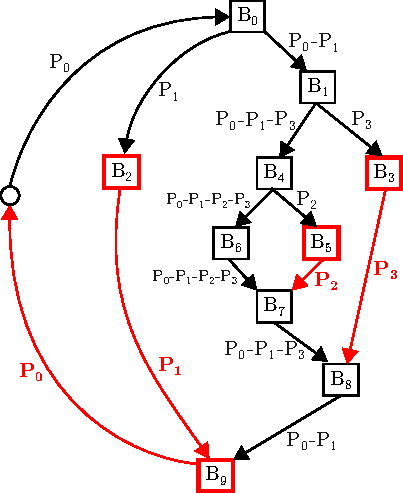
\includegraphics[scale=1]{figs/cfg-example.pdf}\\\vspace{1ex}
  \resizebox{0.8\textwidth}{!}{
  %\scalebox{0.8}{
     \begin{minipage}{0.5\textwidth}
     Instrumented value for each probe $P_i$:
     \begin{align*}
     \omega(P_0) &= w(B_0) + w(B_1) + w(B_4) + w(B_6) + w(B_7) + w(B_8) + w(B_9)\\
     \omega(P_1) &= w(B_2) - w(B_1) - w(B_4) - w(B_6) - w(B_7) - w(B_8)\\
     \omega(P_2) &= w(B_5) - w(B_6)\\
     \omega(P_3) &= w(B_3) - w(B_4) - w(B_6) - w(B_7)
     \end{align*}
     \end{minipage}
  }
}
  \caption{Example of a CFG with its minimum spanning tree in black and the
   basic blocks highlighted in red represent the instrumented basic blocks with
   the placement of the probes.}
  \label{fig:cfg-example}
\end{figure}

In contrast to the naive instrumentation where each basic block records only its own amount of work, with the optimal profiling, the instrumented basic blocks need to record an aggregated value of work that represents a path in the CFG.
These values are constructed with some instrumented basic blocks speculatively assuming some paths while other probes correct when these assumptions are wrong (see for example $w(P_0)$ and $w(P_1)$ in Figure~\ref{fig:cfg-example}).

%\begin{algorithm}[h]
%  \caption{Pseudocode of the data-flow analysis for assigning the values computed
%  in each probe of the instrumentation for the profiling of the work metric.}
%  \label{alg:populateEdgeInfo}
%  \begin{algorithmic}
%    \Function{\textrm{populateEdgeInfo}}{$G$}
%    
%    \For{\textbf{each} $e \in $ \textrm{instrumentedEdges}($G$) }
%       \State $B_I \gets $ \textrm{instrumentedBlock}($e$)
%       \State $inc[e] \gets \{ B_I \}$
%       \State $dec[e] \gets \{ \}$
%       \State $known[e] \gets $ \textbf{true}
%    \EndFor
%
%    \State $changed \gets $ \textbf{true}
%    \While{$changed$}
%       \State $changed \gets $ \textbf{false}
%	   \For{\textbf{each} $B \in V(G)$}
%          \State $uIn \gets $ \textrm{unknownIn}($known, G, B$)
%          \State $uOut \gets $ \textrm{unknownOut}($known, G, B$)
%		  \If{$uIn=0$ \textbf{and} $uOut=1$}
%             \State $changed \gets $ \textbf{true}
%		     \State $incOut \gets \{\}$
%			 \State $decOut \gets \{\}$
%		     \For{$B_p\in$ \textrm{predecessors}($G, B$)}
%			    \State $incOut \gets incOut \bigcup inc[(B_p,B)]$
%			    \State $decOut \gets decOut \bigcup dec[(B_p,B)]$
%			 \EndFor
%		     \For{$B_s\in$ \textrm{successors}($G, B$)}
%			    \State $incOut \gets incOut \cup dec[(B,B_s)]$
%			    \State $decOut \gets decOut \cup inc[(B,B_s)]$
%			 \EndFor
%		     \For{$B_s\in$ \textrm{successors}($G, B$)}
%			    \If{\textbf{not} $known[(B,B_s)]$}
%			       \State $inc[(B,B_s)] \gets incOut\setminus{decOut}$
%			       \State $dec[(B,B_s)] \gets decOut\setminus{incOut}$
%			       \State $known[(B,B_s)] \gets$ \textbf{true}
%				\EndIf
%			 \EndFor
%		  \EndIf
%		  \If{$uIn=1$ \textbf{and} $uOut=0$}
%             \State $changed \gets $ \textbf{true}
%		     \State $incIn \gets \{\}$
%			 \State $decIn \gets \{\}$
%		     \For{$B_s\in$ \textrm{successors}($G, B$)}
%			    \State $incIn \gets incIn \cup inc[(B,B_s)]$
%			    \State $decIn \gets decIn \cup dec[(B,B_s)]$
%			 \EndFor
%		     \For{$B_p\in$ \textrm{predecessors}($G, B$)}
%			    \State $incIn \gets incIn \bigcup dec[(B_p,B)]$
%			    \State $decIn \gets decIn \bigcup inc[(B_p,B)]$
%			 \EndFor
%		     \For{$B_p\in$ \textrm{predecessors}($G, B$)}
%			    \If{\textbf{not} $known[(B_p,B)]$}
%			       \State $inc[(B_p,B)] \gets incIn\setminus{decIn}$
%			       \State $dec[(B_p,B)] \gets decIn\setminus{incIn}$
%			       \State $known[(B_p,B)] \gets$ \textbf{true}
%				\EndIf
%			 \EndFor
%		  \EndIf
%	   \EndFor
%    \EndWhile
%    \EndFunction
%  \end{algorithmic}
%\end{algorithm}

\begin{lstlisting}[caption={Pseudocode of the data-flow analysis for assigning the values computed
  in each probe of the instrumentation for the profiling of the work metric.}, label={lst:populateEdgeInfo}, float]
// Inputs: CFG with the known edges flows of the chords
// Output: Updated CFG with all edge flows
populateEdgeInfo(G) {
  //the instrumented edges are the only known edge flows
  for e in instrumentedEdges(G):
    B = instrumentedBlock(e)
    inc[e] = set{B}
    dec[e] = set{}
    knownInfo[e] = true

  changed = true
  while changed:
    changed = false
    for B in G.vertices():
      unIN = count( G.unknownIncomingEdges(B,knownInfo) )
      unOUT = count( G.unknownOutgoingEdges(B,knownInfo) )
      if unIN==0 and unOUT==1:
        //sum known incoming and outgoing edges in B
        incSum = set{}
        decSum = set{}
        for predB in G.predecessors(B):
          incSum = incSum union dec[G.getEdge(predB, B)]
          decSum = decSum union inc[G.getEdge(predB, B)]
        for succB in G.successors(B):
          incSum = incSum union inc[G.getEdge(B, succB)]
          decSum = decSum union dec[G.getEdge(B, succB)]
        //update unknown outgoing edge in B with incSum and decSum
        e = G.getUnknownOutgoingEdge(B,knownInfo)
        inc[e] = incSum-decSum
        dec[e] = decSum-incSum
        knownInfo[e] = true
        changed = true
      if unIN==1 and unOUT==0:
        //sum known incoming and outgoing edges in B
        incSum = set{}
        decSum = set{}
        for predB in G.predecessors(B):
          incSum = incSum union inc[G.getEdge(predB, B)]
          decSum = decSum union dec[G.getEdge(predB, B)]
        for succB in G.successors(B):
          incSum = incSum union dec[G.getEdge(B, succB)]
          decSum = decSum union inc[G.getEdge(B, succB)]
        //update unknown incoming edge in B with incSum and decSum
        e = G.getUnknownIncomingEdge(B,knownInfo)
        inc[e] = incSum-decSum
        dec[e] = decSum-incSum
        knownInfo[e] = true
        changed = true
}\end{lstlisting}

Because the algorithm for the optimal placement of the probes is proved to uniquely compute the block frequencies by propagating the probe counts, we adapt this algorithm (see \lstlistingname~\ref{lst:populateEdgeFlows}) in order to compose the aggregated values that will be instrumented in each probe, based on our model of computational work, $\Delta W$, derived from the basic block frequencies (see Section~\ref{sec:metric}).
We perform a similar propagation of the probes in a symbolic fashion, as illustrated in Figure~\ref{fig:cfg-example}.
This symbolic propagation of the probes is implemented by the data-flow analysis described in \lstlistingname~\ref{lst:populateEdgeInfo}, and the final aggregated values are extracted from the edge information as described by \lstlistingname~\ref{lst:instrValue}.

The data-flow analysis in \lstlistingname~\ref{lst:populateEdgeInfo} keeps two sets for each edge, namely, the increment and the decrement sets.
We consider that both sets represent the \textit{edge expressions} shown in Figure~\ref{fig:cfg-example}, for which we define a \textit{symbolic sum} by computing the union of the increment and decrement sets, respectively, with the appropriate cancellation of common elements.
This data-flow analysis is based on the invariant that the symbolic sum of all the incoming edges must equals the symbolic sum of the outgoing edges.
For example, the symbolic sum of the incoming edges of the basic block $B_8$ is $P_0 - P_1$, where $P_3$ is cancelled out.

%By construction, the \textit{symbolic experssions} of a basic block, i.e., the \textit{symbolic sum} of the incoming edges (or outgoing edges) of a basic block, has the following properties:
%\begin{enumerate}
%\item Probes in the increment set either (post-)dominates or is (post-)dominated by the given basic block;
%\item Probes in the decrement set are (post-)dominated by the probes in the increment set;
%\item Probes in the decrement set and the given basic block are in exclusive paths from the virtual node of the CFG to the (post-)dominators in the increment set;
%\end{enumerate}
%From property (1) it follows that whenever the given basic block is executed, exactly one of the probes in the increment set is executed.
%From properties (2) and (3), it follows that whenever a probe in the decrement set is executed, although the given basic block is not executed, one of the probes in the decrement set is executed.

\lstlistingname~\ref{lst:instrValue} reads the edge information for each basic block by computing the symbolic sum of their respective incoming edges (or outgoing edges).
From these \textit{edge expressions}, we are able to compose the aggregated value of the probes.
The positive terms in the edge expression of a basic block indicate that the amount of work of this basic block will be incremented in the probes represented by these positive terms, similarly, the negative terms indicate that the amount of work of this basic block will be decremented in the probes represented by these negative terms.
For example, because the edge expression for the basic block $B_8$ is $P_0 - P_1$, the amount of work of $B_8$, denoted by $w(B_8)$, is incremented in probe $P_0$ and decremented in $P_1$.

%\begin{algorithm}[h]
%  \caption{Pseudocode that describes how the edge information is used in order to extract the value that will be computed in a given instrumented basic block $B_I$. This algorithm could equally be implemented based on the predecessors.}
%  \label{alg:instrValue}
%  \begin{algorithmic}
%    \Function{\textrm{instrValue}}{$G, B_I, inc, dec$}
%	\State $v \gets 0$
%    \For{\textbf{each} $B \in V(G)$}
%	   \State $inc_B \gets \{\}$
%	   \State $dec_B \gets \{\}$
%%	   \For{$B_p\in$ \textrm{predecessors}($G, B$)}
%%	      \State $inc_B \gets inc_B \bigcup inc[(B_p,B)]$
%%	      \State $dec_B \gets dec_B \bigcup dec[(B_p,B)]$
%%	   \EndFor
%	   \For{$B_s\in$ \textrm{successors}($G, B$)}
%	      \State $inc_B \gets inc_B \bigcup inc[(B,B_s)]$
%	      \State $dec_B \gets dec_B \bigcup dec[(B,B_s)]$
%	   \EndFor
%	   \If{ $B_I \in inc_B\setminus{dec_B}$}
%	      \State $v \gets v + w(B)$
%	   \EndIf
%	   \If{ $B_I \in dec_B\setminus{inc_B}$}
%	      \State $v \gets v - w(B)$
%	   \EndIf
%	\EndFor
%    \Return $v$
%    \EndFunction
%  \end{algorithmic}
%\end{algorithm}

\begin{lstlisting}[caption={Pseudocode that describes how the edge information is used in order to extract the value that will be computed in a given instrumented basic block $B_I$. This algorithm could equally be implemented based on the predecessors.}, label={lst:instrValue}, float]
// Inputs: 1) CFG with the known edges flows of the chords
//         2) Basic block targeted for probing
// Output: Work value to be incremented by the given probe B
instrValue(G, B, inc, dec) {
  value = 0
  for B in G.vertices():
    incB = set()
    decB = set()
    for succB in G.successor(B):
      incB = incB union inc[ G.getEdge(B, succB) ]
      decB = decB union dec[ G.getEdge(B, succB) ]
    if B in (incB - decB):
      value = value + w(B)
    if B in (decB - incB):
      value = value - w(B)
  return value
}
\end{lstlisting}

\section{Code Generation for the Instrumentation Probes}

This section describes the code generator for the work instrumentation.
Once we have the placement of the probes as well as the aggregated value computed for each probe, we insert the appropriate instructions for the probes of the work profiling.
Because the instrumented code is assumed to be generated before optimising the code, the code generator has a straightforward code generation process.
It produces the code for the probes using a local variable as it tends to improve optimisation opportunities.
This variable acts as the local accumulator that will eventually be incremented into the global work counter.

For every function, the code generator allocates memory on the stack frame for the local work variable.
In LLVM, allocated memory on the stack is automatically released when the function returns, therefore there is no need to generate code for that purpose.
Afterwards, the local work variable is set to zero.

\begin{lstlisting}[language=llvm,style=nasm,caption={Code for the entry point of a function.}, label={lst:instr_entry_point}]
  %local.work = alloca i32
  store i32 0, i32* %local.work
\end{lstlisting}

For every probe, the code generator produces memory access operations in addition to the actual increment of the local work counter.
The value incremented to the local counter is the value computed by \lstlistingname~\ref{lst:instrValue}.

\begin{lstlisting}[language=llvm,style=nasm,caption={Code for a probe that increments the local work counter.}, label={lst:instr_probe}]
  %r1 = load i32, i32* %local.work
  %r2 = add i32 %r1, 8
  store i32 %r2, i32* %local.work
\end{lstlisting}

Because it produces instrumentation code using a local variable, eventually this local variable needs to be incremented into the global counter.
This is performed at every exit point of the function, even if the basic block with the exit point was not selected for having a probe.
For every exit point of the function, the code generator produces simple memory access operations that load the current values of both the local and the global counters, adds them together, and finally updates the global counter.

\begin{lstlisting}[language=llvm,style=nasm,caption={Code at an exit point of a function.}, label={lst:instr_exit_point}]
  %r1 = load i32, i32* %local.work
  %r2 = load i32, i32* @__work_counter
  %r3 = add i32 %r1, %r2
  store i32 %r3, i32* @__work_counter
\end{lstlisting}

For the special case where a probe belongs to a basic block which is also an exit point of the function, the code generator leverages from this scenario to produce a code for the probe that works in collaboration with the update of the global counter.

\begin{lstlisting}[language=llvm,style=nasm,caption={Code for a probe that increments the local work counter and also updates the global counter at an exit point of a function.}, label={lst:instr_probe_exit_point}]
  %r1 = load i32, i32* %local.work
  %r2 = add i32 %r1, 273
  %r3 = load i32, i32* @__work_counter
  %r4 = add i32 %r2, %r3
  store i32 %r4, i32* @__work_counter
\end{lstlisting}

After optimisations, the instrumented code can benefit from some of the transformations.
For example, the optimisation pass for promoting memory to register (\texttt{-mem2reg}) is able to eliminate the local variable such that the local work counter is only kept in registers.
The only explicit access to memory is performed when updating the global work counter.

\begin{lstlisting}[language=llvm,style=nasm,caption={An illustrative example of how \texttt{-mem2reg} can optimise the instrumented code.}, label={lst:instr_opt_probe}]
  ...
  ;If probes from multiple paths reach a given point,
  ;a phi operation is used for selecting the appropriate value.
  ;Furthermore, the initial store of 0 is unnecessary.
  %r1 = phi i32 [ 0, %entry ], [ %r2, %for.inc ]
  ...
  ;If there is only one value that reaches a given point,
  ;this value can be directly used.
  %r3 = add i32 %r1, 273
  %r4 = load i32, i32* @__work_counter
  %r5 = add i32 %r3, %r4
  store i32 %r5, i32* @__work_counter
\end{lstlisting}

\section{Relaxed Instrumentation}

Although the optimal instrumentation significantly reduces the profiling overhead when compared to the naive instrumentation, from an average overhead of 79\% to 13\%, in some critical cases, even the optimal instrumentation can have an overhead of about 70\% (see benchmark \texttt{adpcm\_d} in Figure~\ref{fig:overhead-O3}).
In order to further reduce the overhead in these critical cases, we propose a relaxed instrumentation by trading off accuracy and overhead.
While the optimal placement of probes tries to place probes in edges that are less likely to be executed, the relaxation focus on removing probes that are more likely to be executed.

\begin{figure}[h]
  \centering
  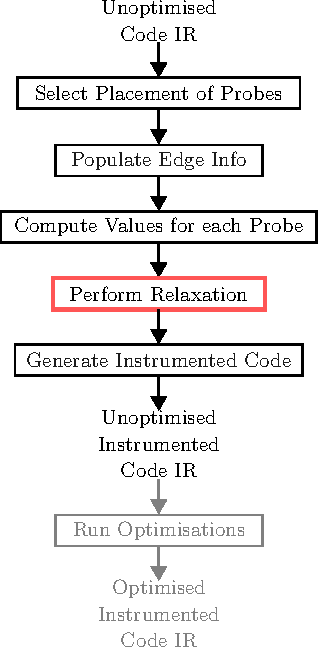
\includegraphics[scale=0.9]{figs/relax-instr-diagram.pdf}
  \caption{Diagram.}
  \label{fig:relax-instr-diagram}
\end{figure}

%\begin{figure*}[htb]
%    \centering
%    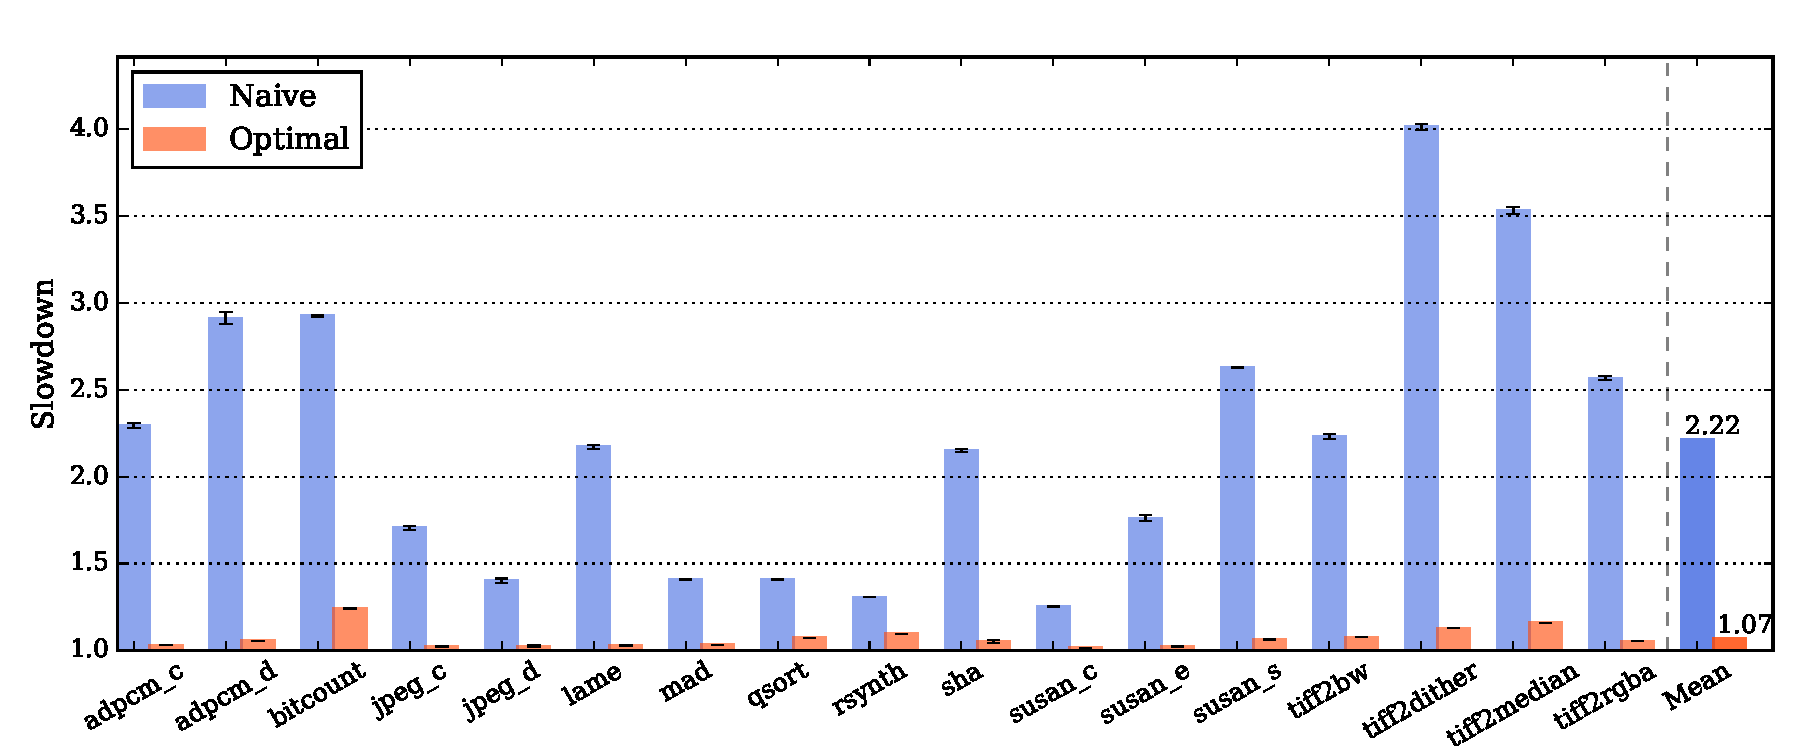
\includegraphics[width=\textwidth]{figs/overhead-O0.pdf}
%    \caption{Comparison between the naive and optimal instrumentation
%              with no compiler optimisation.}
%    \label{fig:overhead-O0}
%\end{figure*}

%Define an DAG of a CFG as a directed graph which may contain cycles if they have known constant trip counts.
Figure~\ref{fig:relax-instr-diagram} shows an overview of the relaxed instrumentation algorithm.
The highlighted step is introduced by the relaxed instrumentation on top of the previously defined optimal work instrumentation algorithm.
The relaxed instrumentation performs a post-processing on the resulting instrumentation of the optimal algorithm.
The relaxation starts by extracting DAGs (directed acyclic graphs) from the CFG, as illustrated in Figure~\ref{fig:cfg-relax-example}.
The algorithm extracts all the subgraphs that represent a loop or the outer most region of the function.
These subgraphs are transformed into DAGs by ignoring the back edge and also by considering that any loop within the subgraph is never executed, i.e., only the headers of the inner loops are actually included into the DAG.
Figure~\ref{fig:cfg-relax-example} shows a CFG partitioned into two DAGs (consider only basic blocks and edges completely inside the yellow and green boundaries).
%
%LLVM has a Scalar Evolution Analysis which is used primarily to analyse expressions involving induction variables in loops~\cite{pop05}.
%An induction variable is a variable that is increased or decreased by a fixed amount on every iteration of a loop or is a linear function of another induction variable.
%
%This Scalar Evolution Analysis provides a way to compute \textit{small} constant trip counts (where \textit{small} is defined by a threshold).

\begin{figure}[h]
  \centering
  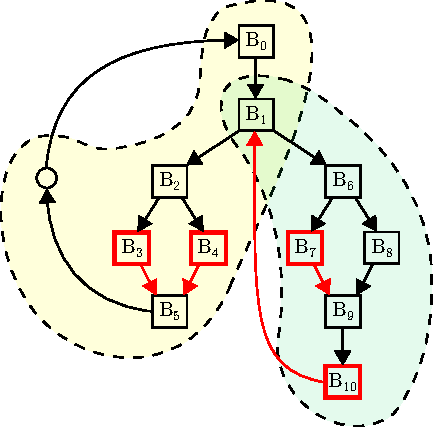
\includegraphics[scale=1]{figs/cfg-relax-example.pdf}
  \caption{Example of a CFG containing a loop and its decomposition into DAGs when applying the relaxation.
           The DAGs are the subgraphs within the dashed boundaries.}
  \label{fig:cfg-relax-example}
\end{figure}


\begin{lstlisting}[caption={Optimal placement of probes for block frequency.}, label={lst:instrumentCFG}]
// Input: CFG	
relaxInstrumentation(G) {
  for loop in G:
     DAG = colapseInnerLoops(loop)
     relaxInstrumentedDAG(DAG)
  DAG = colapseInnerLoops(G)
  relaxInstrumentedDAG(DAG)
}
\end{lstlisting}

For every DAG with a set of probes $\{P_0, P_1, \ldots, P_k\}$, we relax the profiling accuracy by selecting a subset of the probes to be removed, subject to the maximum allowed percentage error, $M$.

We model the relaxation as a 0-1 Knapsack problem:
\begin{equation*}
\begin{aligned}
& \textrm{maximise }\quad \sum_{i=0}^{k} f(P_i)x_i \\
& \textrm{subject to }\quad \sum_{i=0}^{k} \varepsilon(P_i)x_i \leq M
\end{aligned}
\end{equation*}
\[
x_i\in\{0,1\}, i\in\{0,\ldots,k\}
\]
where $f(P_i)$ is the execution frequency of probe $P_i$, $x_i$ denotes the probes selected for removal, and $\varepsilon(P_i)$ is the percentage error of removing probe $P_i$ relative to the minimum work value possible to compute in the DAG, i.e., if $m$ is the minimum amount of work possible to be computed when executing the DAG, then $\varepsilon(P_i) = \frac{\omega(P_i)}{m}$.
Because the percentage error is computed based on the path with the minimum amount of work, $\varepsilon(P_i)$ represents the maximum error possible that would be incurred when removing probe $P_i$.
Furthermore, by constraining the percentage error of every DAG below a given threshold we guarantee that the final error of the relaxation will always be bounded by the threshold, as demonstrated by Proposition~\ref{prop:relax-bound}.

\begin{prop}\label{prop:relax-bound}
Let $n_i$ be the number of times a given DAG $i$ is executed, $r_i$ be the total relaxation (amount of work removed) in DAG $i$, and $m_i$ be its minimum amount of work.
If $\frac{r_i}{m_i} \leq M$ for every $i$,
then the final error of the relaxation will always be bounded by the same threshold.
\end{prop}
\begin{proof}
We can model the overall error of the relaxation as:
\[
1 - \frac{n_1(m_1 - r_1) + n_2(m_2 - r_2) + \ldots + n_k(m_k - r_k) + c}{n_1m_1 + n_2m_2 + \ldots + n_km_k + c}
\]
That is,
%\begin{equation*}
\begin{gather*}
 1 - \frac{n_1m_1 + n_2m_2 + \ldots + n_km_k + c}{n_1m_1 + n_2m_2 + \ldots + n_km_k + c} + \frac{n_1r_1 + n_2r_2 + \ldots + n_kr_k}{n_1m_1 + n_2m_2 + \ldots + n_km_k + c} = \\
 \frac{n_1r_1 + n_2r_2 + \ldots + n_kr_k}{n_1m_1 + n_2m_2 + \ldots + n_km_k + c}
\end{gather*}
%\end{equation*}
If $\frac{r_j}{m_j}$ is the maximum ratio $\frac{r_i}{m_i}$ for every $i$, then
\begin{equation*}
\begin{aligned}
 \frac{n_1r_1 + n_2r_2 + \ldots + n_kr_k}{n_1m_1 + n_2m_2 + \ldots + n_km_k + c} &\leq\\
 \frac{n_1r_j + n_2r_j + \ldots + n_kr_j}{n_1m_j + n_2m_j + \ldots + n_km_j + c} &\leq\\
 \frac{n_1r_j + n_2r_j + \ldots + n_kr_j}{n_1m_j + n_2m_j + \ldots + n_km_j} & 
\end{aligned}
\end{equation*}
If $N = max\{n_i$ for every $i\}$, then
\begin{equation*}
\begin{aligned}
 \frac{n_1r_j + n_2r_j + \ldots + n_kr_j}{n_1m_j + n_2m_j + \ldots + n_km_j} &\leq\\
 \frac{Nr_j + Nr_j + \ldots + Nr_j}{Nm_j + Nm_j + \ldots + Nm_j} &=\\
 \frac{Nkr_j}{Nkm_j} = \frac{r_j}{m_j} &\leq M
\end{aligned}
\end{equation*}
\end{proof}


\begin{lstlisting}[caption={Optimal placement of probes for block frequency.}, label={lst:instrumentCFG}]
// Input: CFG	
relaxInstrumentedDAG(DAG){
   P = ProbesIn(DAG)
   m = minWork(DAG,P)
   K = createKnapsackModel(P,m)
   Bag = solveKnapsack(K)
   for B in (P-Bag):
     removeProbe(B)
}
\end{lstlisting}

The necessary block-frequency information for optimising both the placement of probes can be acquired from profiles of previous executions of the program or by a static heuristic of the CFG during compilation.

For our experiments, we implemented two solvers for the 0-1 Knapsack problem:
the optimal brute-force solver;
the greedy heuristic based on sorting the items~\citep{dantzig57}.
We use the brute-force solver for DAGs with a small number of probes and the greedy heuristic when the number of probes is greater than a threshold.
Some of the benchmarks have DAGs with several hundreds of probes, which could result in a long compilation time.

\section{Whole Program Relaxation}

In some cases, the proposed relaxation can be very conservative, because it considers the static error of removing probe $P_i$ relative to the minimum work possible of a DAG, in order to be able to guarantee that the dynamic error will be bounded by a given threshold.
This conservatism can be overly restrictive in some cases, resulting in a negligible overhead reduction but also causing only negligible dynamic error to the work profiling.

In some cases, this overly restrictive conservatism may be unnecessary.
For these cases, we propose an adapted version of the relaxation algorithm that operates on the whole program.
Traditionally, compilers optimisations are performed on the function-level, or at best on a per module basis.
Whole program optimisation (WPO) means that the compiler considers all compilation units of the program and optimises them using the combined knowledge of how they are used together.

The whole program relaxation works by using block-frequency profiling from previous executions.
By having this profiling information, the \textit{whole program relaxation} is able to compute the error of removing a given probe in terms of the whole program's execution,
and then use this error values for selecting a subset of all the probes to be removed.

For a program with a set of probes $\{P_0, P_1, \ldots, P_k\}$, we model the whole program the relaxation as the following 0-1 Knapsack problem:
\begin{equation*}
\begin{aligned}
& \textrm{maximise }\quad \sum_{i=0}^{k} f(P_i)x_i \\
& \textrm{subject to }\quad \sum_{i=0}^{k} \varepsilon(P_i)x_i \leq M
\end{aligned}
\end{equation*}
\[
x_i\in\{0,1\}, i\in\{0,\ldots,k\}
\]
where $f(P_i)$ is the execution frequency of the instrumented basic block $P_i$, $x_i$ denotes the probes selected for removal, $M$ is the error threshold, and $\varepsilon(P_i)$ is the percentage error of removing probe $P_i$ relative to the profiled global work, i.e.,
if $\Delta W$ is the work value for the whole program's execution, computed from the basic block frequencies profiled from previous executions, the error for a given probe $P_i$ is
\[
\varepsilon(P_i) = \frac{\omega(P_i)f(P_i)}{\Delta W}.
\]

Contrary to the per DAG relaxation, the whole program relaxation is not guaranteed to be bounded by the error threshold $M$,
as it is dependent on the representativity%representativeness
 of the profiling information that was provided.



\chapter{Experimental Evaluation}\label{chap:eval}

In this chapter, we discuss our experimental evaluation.
First, we describe the benchmarks with datasets used in the experiments.
Afterwards, we discuss our results concerning the instrumentations for profiling our work metric.
Finally we present results of the online {\itercomp}.

We implemented the instrumentations in LLVM 4.0\footnote{The implementation of the work profiling in LLVM is available at: \url{https://github.com/rcorcs/llvm-work-instr}.}.
All experiments use the Clang/LLVM compiler suite.
The target platform is a Linux-4.4.27 system with an Intel Core i7-4770 3.40GHz Skylake~CPU with 16~GiB RAM.

\section{Benchmarks and Datasets} \label{sec:benchmarks}

%{\Itercomp} is essentially based on repeatedly trying out a large number of compiler optimisations until the best combination of compiler optimisations is found for a particular program.
%Our main goal is to speed up {\itercomp} while targeting optimal performance across large input datasets.

For the experimental evaluation, we have used a subset of the \textit{KDataSets} benchmark suite, which is the same benchmark and dataset suite used by \cite{chen10,chen12a}.
The KDataSets contains 1000 different inputs for each one of its benchmark programs.
These benchmarks cover a broad spectrum of application scenarios, ranging from simple embedded signal-processing tasks to common mobile-phone and desktop tasks.
The different inputs try to capture distinct characteristics in terms of workload sizes and how these workloads exercise different control flow paths.
A summary of the benchmarks and dataset suite is shown in Table~\ref{tab:kdatasets}.

\begin{table}[h]
\centering
\scalebox{.8}{
\begin{tabular}{|c|c|c|c|}
\hline
\textbf{Program} & \textbf{LOC}    & \textbf{Input file size}            & \textbf{Input description}              \\ \hline % Domain
qsort         & 154    & 32K-1.8M                   & 3D coordinates                 \\ \hline
jpeg\_d       & 13501  & 3.6K-1.5M                  & JPEG images                    \\ \hline
jpeg\_c       & 14014  & 16K-137M                   & PPM images                     \\ \hline
tiff2bw       & 15477  & \multirow{4}{*}{9K-137M}   & \multirow{4}{*}{TIFF images}   \\ \cline{1-2}
tiff2rgba     & 15424  &                            &                                \\ \cline{1-2}
tiffdither    & 15399  &                            &                                \\ \cline{1-2}
tiffmedian    & 15870  &                            &                                \\ \hline
susan\_c      & 1376   & \multirow{3}{*}{12K-46M}   & \multirow{3}{*}{PGM images}    \\ \cline{1-2}
susan\_e      & 1376   &                            &                                \\ \cline{1-2}
susan\_s      & 1376   &                            &                                \\ \hline
adpcm\_c      & 210    & 167K-36M                   & WAVE audios                    \\ \hline
adpcm\_d      & 211    & 21K-8.8M                   & ADPCM audios                   \\ \hline
lame          & 14491  & 167K-36M                   & WAVE audios                    \\ \hline
rsynth        & 4111   & 0.1K-42M                   &  Text files                    \\ \hline
sha           & 197    & 0.6K-35M                   & Files of any format            \\ \hline
\rowcolor{gray!20}
bitcount      & 460    &  -                         & Numbers: random                \\ \hline
\rowcolor{gray!20}
dijkstra      & 163    & 0.06K-4.3M                 & Adjacency matrices             \\ \hline
\rowcolor{gray!20}
patricia      & 290    & 0.6K-1.9M                  & IP and mask pairs              \\ \hline
\rowcolor{gray!20}
mad           & 2358   & 28K-27M                    & MP3 audios                     \\ \hline
\rowcolor{gray!20}
%gsm           & 3806   & 83K-18M                    & Sun/NeXT audios                \\ \hline
ghostscript   & 99869  & 11K-43M                    & Postscript files               \\ \hline
\rowcolor{gray!20}
%ispell        & 6522   & \multirow{3}{*}{0.1K-42M}  & \multirow{3}{*}{Text files}    \\ \cline{1-2}
%rsynth        & 4111   &                            &                                \\ \cline{1-2}
stringsearch  & 338    &  0.1K-42M                 &  Text files                     \\ \hline
\rowcolor{gray!20}
%blowfish\_e   & 863    & 0.6K-35M                   & Files of any format            \\ \hline
%blowfish\_d   & 863    & 0.6K-35M                   & Encrypted files                \\ \hline
%pgp\_e        & 19575  & 0.6K-35M                   & Files of any format            \\ \hline
%pgp\_d        & 19575  & 0.4K-18M                   & Encrypted files                \\ \hline
%rijndael\_e   & 952    & 0.6K-35M                   & Files of any format            \\ \hline
%rijndael\_d   & 952    & 0.7K-35M                   & Encrypted files                \\ \hline
CRC32         & 130    & 0.6K-35M                   & Files of any format            \\ \hline
\rowcolor{gray!20}
bzip2e        & 5125   & 0.7K-57M                   & Files of any format            \\ \hline
\rowcolor{gray!20}
bzip2d        & 5125   & 0.2K-25M                   & Compressed files               \\ \hline
\end{tabular}
}
\caption{Description of the KDataSets with 1000 inputs for each benchmark (Chen~\etal~\cite{chen10,chen12a}).}
\label{tab:kdatasets}
\end{table}

The shaded (grey) benchmarks in Table~\ref{tab:kdatasets} represent the benchmarks used for training the cost model used for computing the weight of the instructions for the work metric.
These same training benchmarks were also used for collecting a fixed set of optimisation sequences for the {\itercomp}.
The remaining (white) benchmarks are used for the experimental evaluation.

\section{Evaluation of the Instrumentation}

In this section, we evaluate the performance of the work instrumentation presented in Chapter~\ref{chap:instr}.
We analyse the optimal work profiling as well as both relaxation algorithms.
%comparing between the optimal and the relaxed instrumentation with different thresholds.
%We organise the evaluation of the instrumentation as follows:

\subsection{Static Evaluation}

We first compare static aspects of the instrumentation algorithms.
The naive instrumentation always has 100\% of the basic blocks instrumented, by definition.
First, we evaluate the optimal work profiling compared to the relaxation algorithm applied per DAG.
Afterwards, we compare these profiling techniques with the whole program relaxation.

Figure~\ref{fig:num-probes} shows the percentage of instrumented basic blocks for the optimal and the relaxed instrumentation with different relaxation thresholds.
While Figure~\ref{fig:num-probes} compares the various instrumentation algorithms in respect of the naive instrumentation, Figure~\ref{fig:num-probes-improvement} shows the improvement of the relaxation algorithm  over the optimal instrumentation.

\begin{figure}[ht]
    \centering
    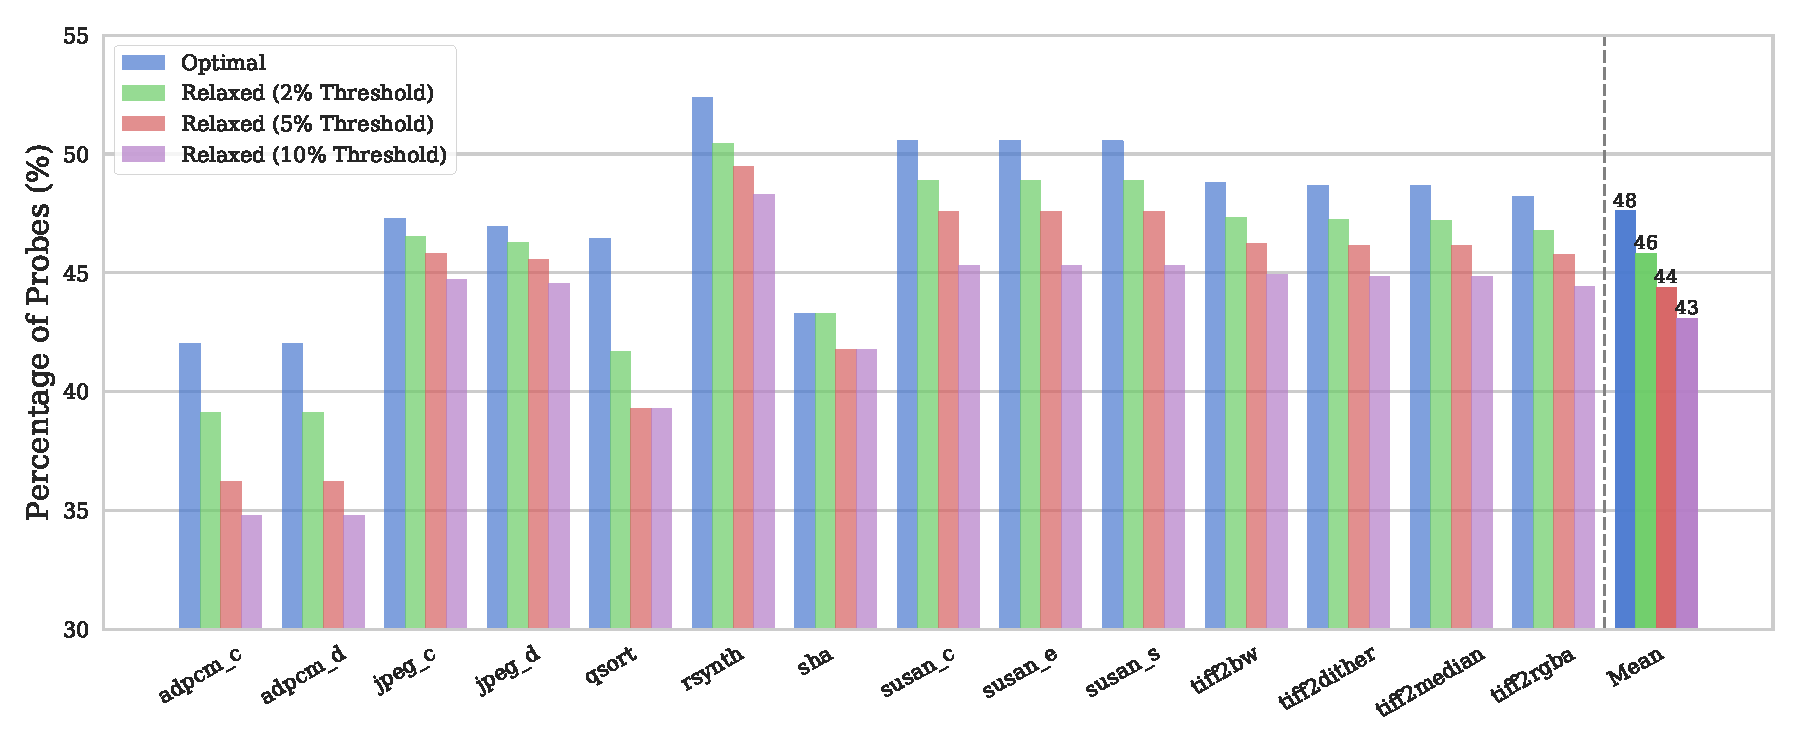
\includegraphics[width=\textwidth]{figs/num-probes.pdf}
    \caption{Percentage of instrumented basic blocks for the optimal and the relaxed instrumentation with different relaxation thresholds.}
    \label{fig:num-probes}
\end{figure}

Even a small threshold of 2\% is able to reduce the number of probes by an average of 5\% compared to the optimal algorithm.
The {\flagstype sha} benchmark was the only benchmark for which a 2\% threshold was not sufficient for further reducing the number of probes.
%With a 10\% threshold the relaxation algorithm was able to improve over the optimal instrumentation by an average of 11\%, in terms of the amount of instrumented basic blocks.
With a 5\% threshold, the relaxation algorithm was able to improve over the optimal instrumentation by an average of 7\%, in terms of the amount of instrumented probes.

\begin{figure}[ht]
    \centering
    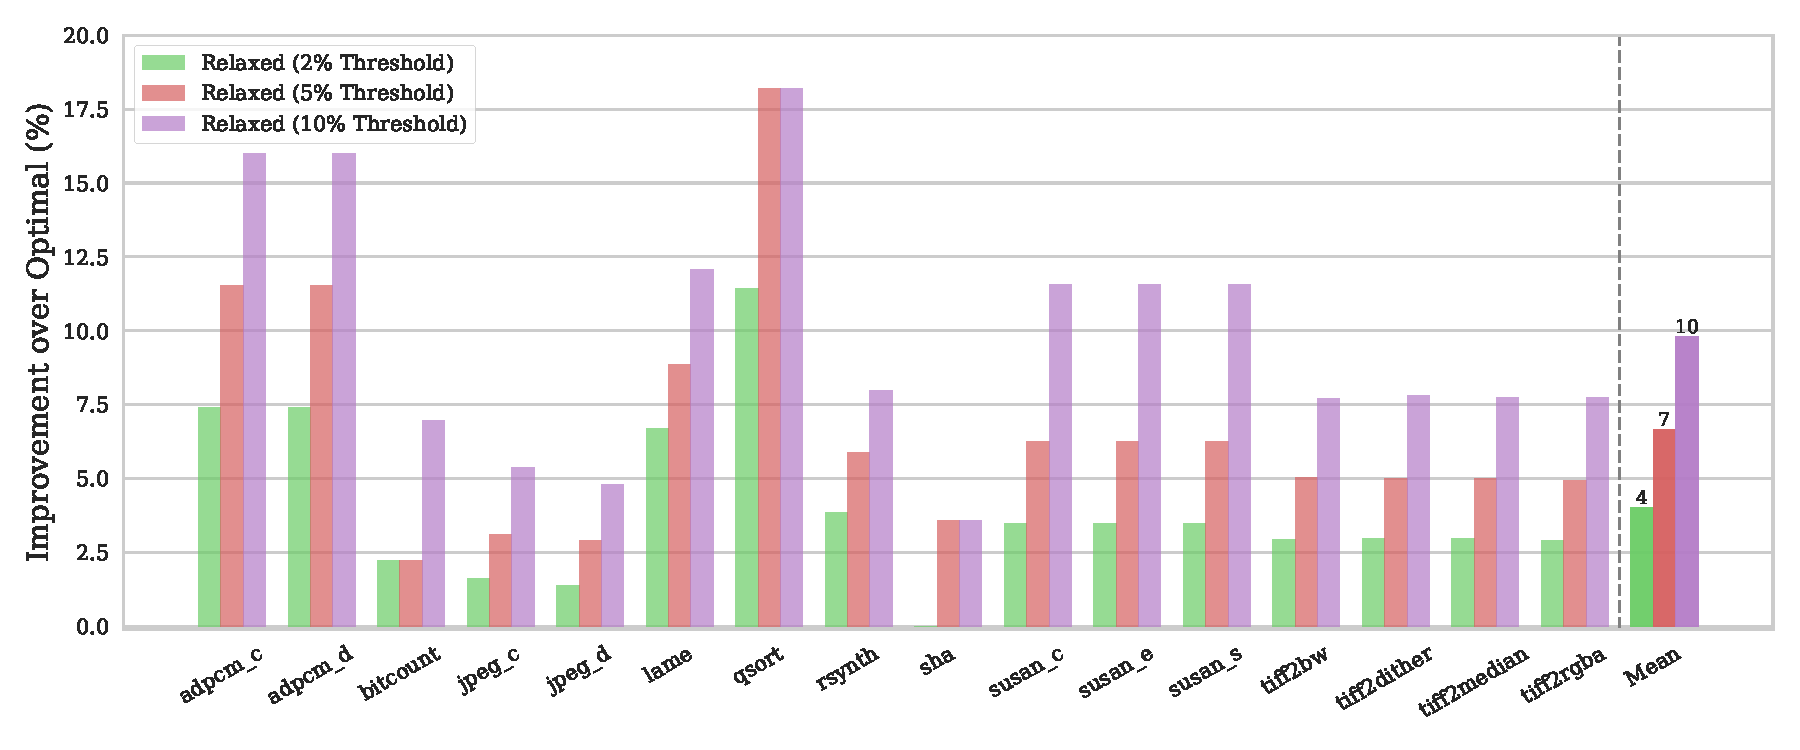
\includegraphics[width=\textwidth]{figs/num-probes-improvement.pdf}
    \caption{Percentage of instrumented basic blocks for the optimal and the relaxed instrumentation with different relaxation thresholds.}
    \label{fig:num-probes-improvement}
\end{figure}

The static errors presented in Figure~\ref{fig:static-instr-error} indicate the amount of error expected by the relaxation algorithm after reducing the number of probes.
This figure shows both the maximum (bars with light colours) and the average (bars with dark colours) static errors observed when relaxing the instrumentation for each DAG of the benchmarks.
Notice that, in most cases, the average static errors are considerably lower than the relaxation threshold, while the maximum static errors are usually close to the threshold.
The average static error shows that in a significant number of DAGs, the relaxation was notably conservative.
This conservatism will be especially evident in the dynamic evaluation.

\begin{figure}[ht]
    \centering
    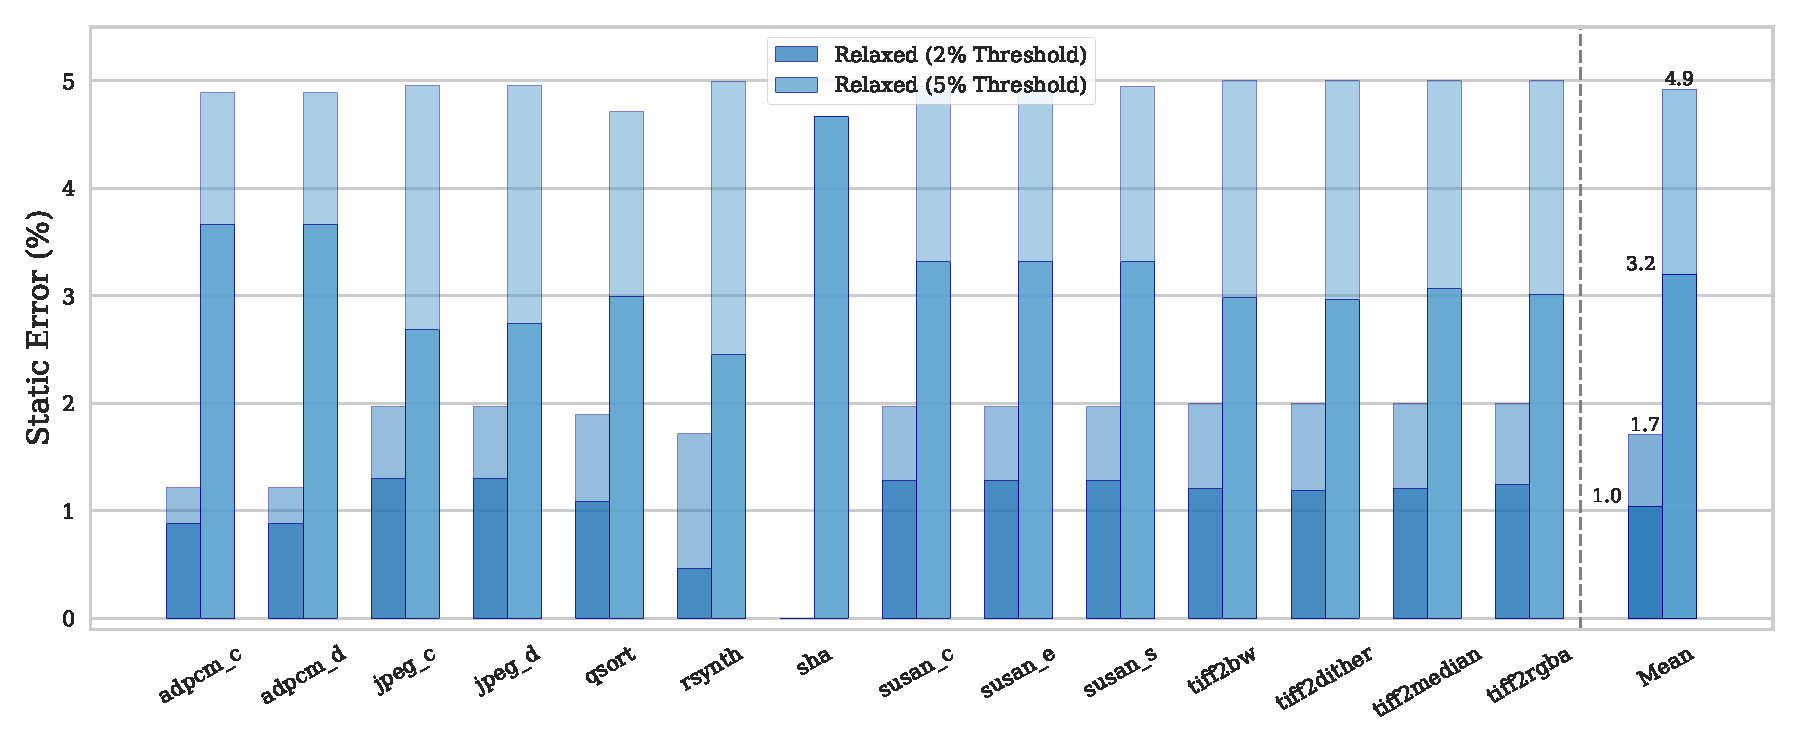
\includegraphics[width=\textwidth]{figs/instr-error.pdf}
    \caption{Average and maximum static error expected for the work profiling, after relaxing the number of probes.}
    \label{fig:static-instr-error}
\end{figure}

The whole program relaxation tries to address this overly conservative aspect of the relaxation algorithm.
Figure~\ref{fig:null-probes-relative-to-optimal} shows the percentage of probes, considering the optimal profiling, that were instrumented in basic blocks that were never executed for randomly selected inputs for each benchmark.
Notice how most of the probes are never executed.
This happens mainly because these benchmarks contain functions which are not called.
For example, the benchmarks {\flagstype adpcm\_c} and {\flagstype adpcm\_d} have the same code, where they differ only in their {\flagstype main} function.
This is also true for the {\flagstype susan\_c}, {\flagstype susan\_e}, and {\flagstype susan\_s} benchmarks.
Therefore, it is natural that some functions are not executed with specific inputs.

\begin{figure}[ht]
    \centering
    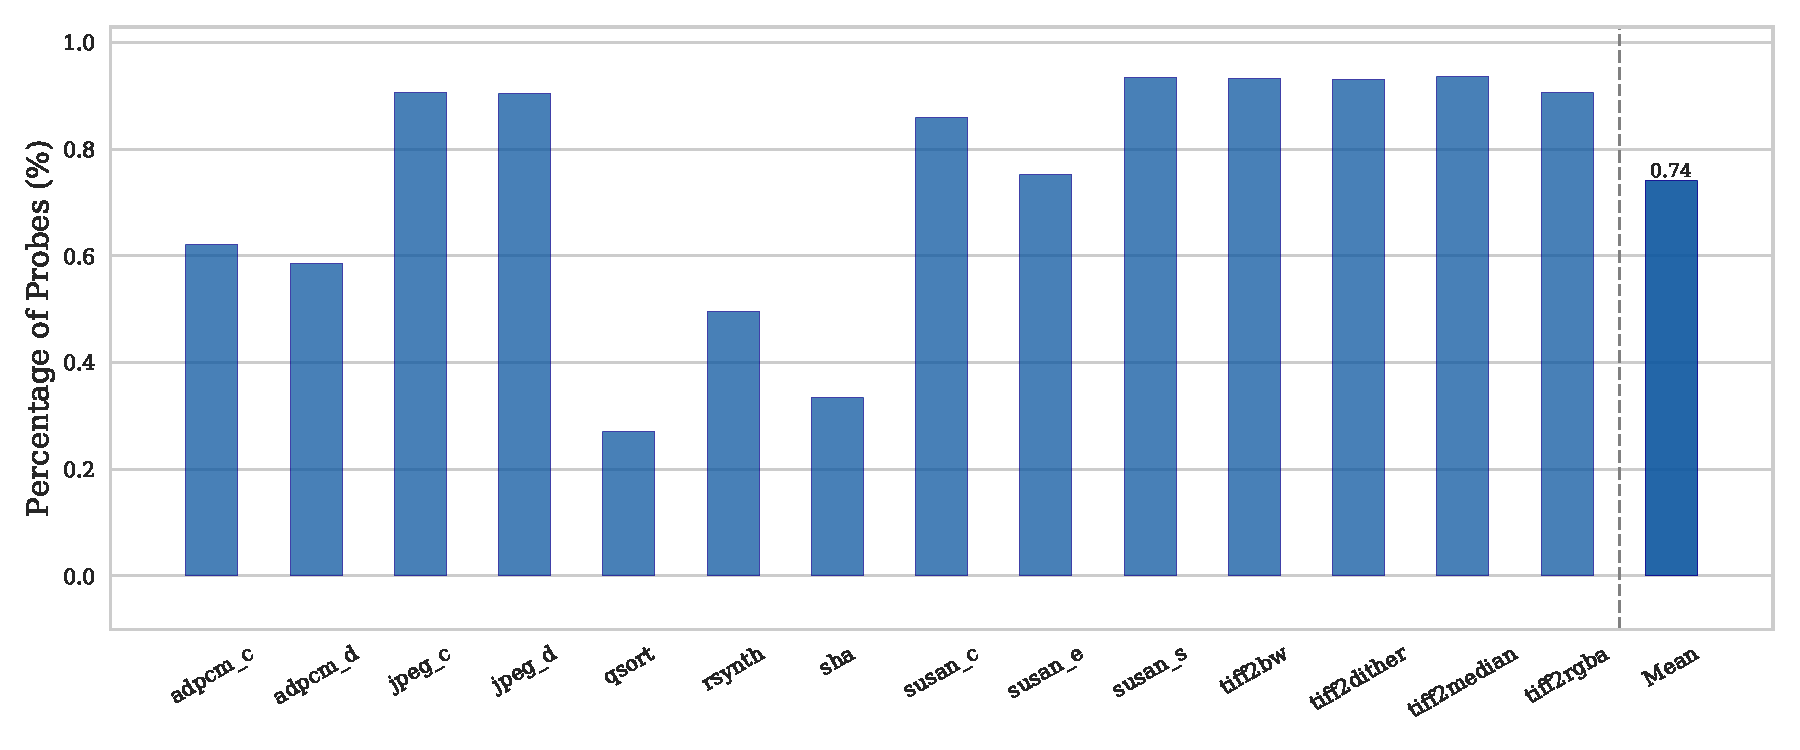
\includegraphics[width=\textwidth]{figs/null-probes-relative-to-optimal.pdf}
    \caption{Percentage of probes instrumented in basic blocks that were never executed, based on a randomly selected input for each benchmark.}
    \label{fig:null-probes-relative-to-optimal}
\end{figure}

\newpage
Figure~\ref{fig:wpo-nonzero-probes-relative-to-optimal} shows the number of instrumented basic blocks, after applying a whole program relaxation with a threshold of 5\%, relative only to the probes from the optimal profiling that are executed, based on a randomly selected input.
We ignore the probes placed in basic blocks that were never executed as they do not affect the measurement of the amount of work.

\begin{figure}[ht]
    \centering
    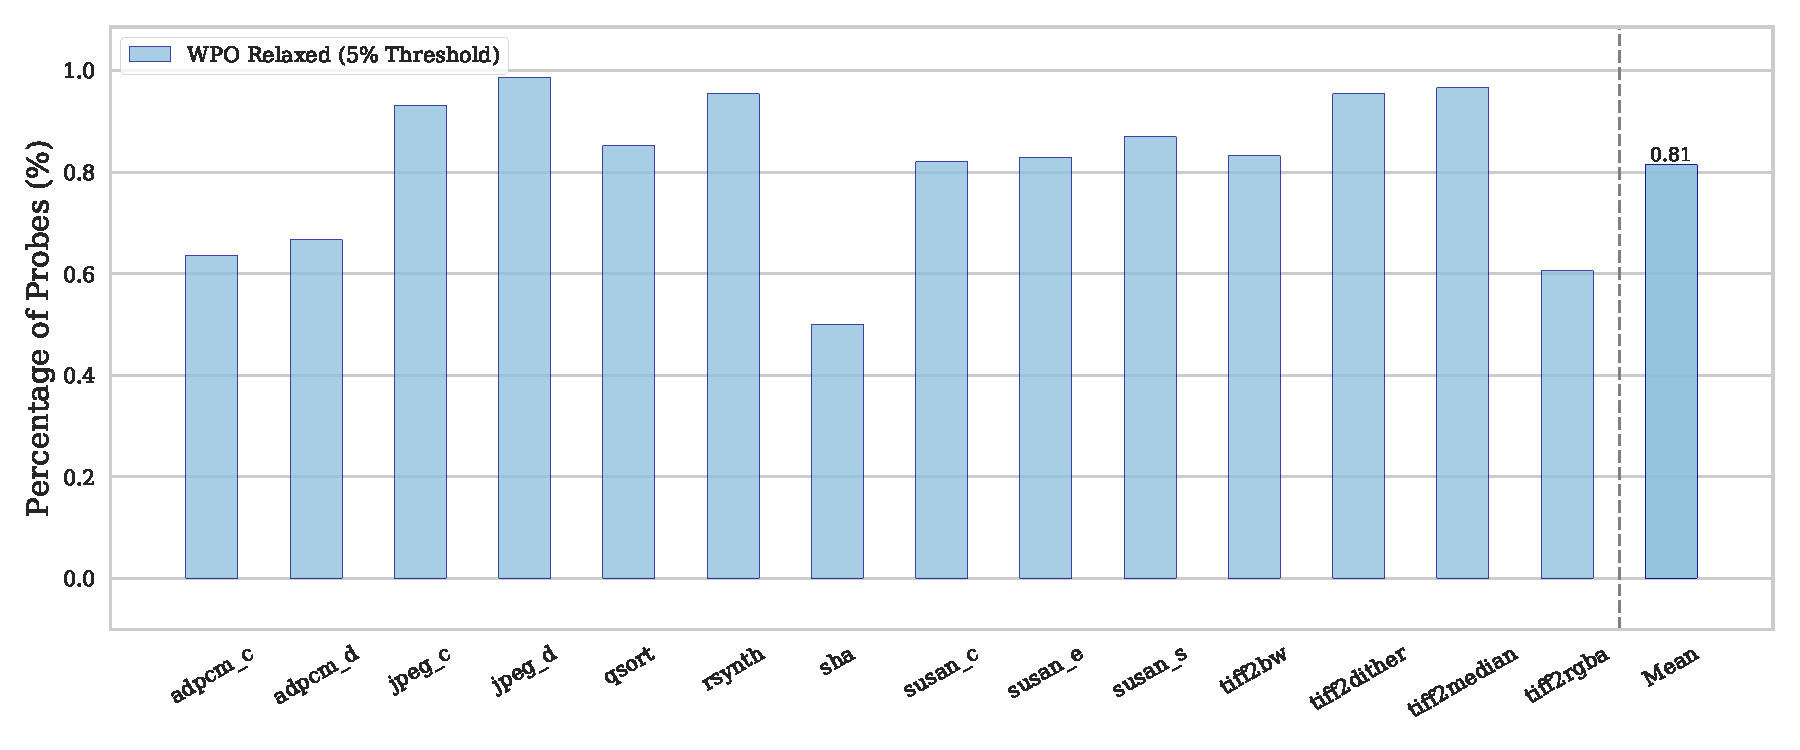
\includegraphics[width=\textwidth]{figs/wpo-nonzero-probes-relative-to-optimal.pdf}
    \caption{Percentage of instrumented basic blocks, after applying a whole program relaxation, relative only to the probes from the optimal profiling that are executed, based on a randomly selected input. In other words, it ignores the probes in basic blocks that were never executed.}
    \label{fig:wpo-nonzero-probes-relative-to-optimal}
\end{figure}

\begin{figure}[h!]
    \centering
    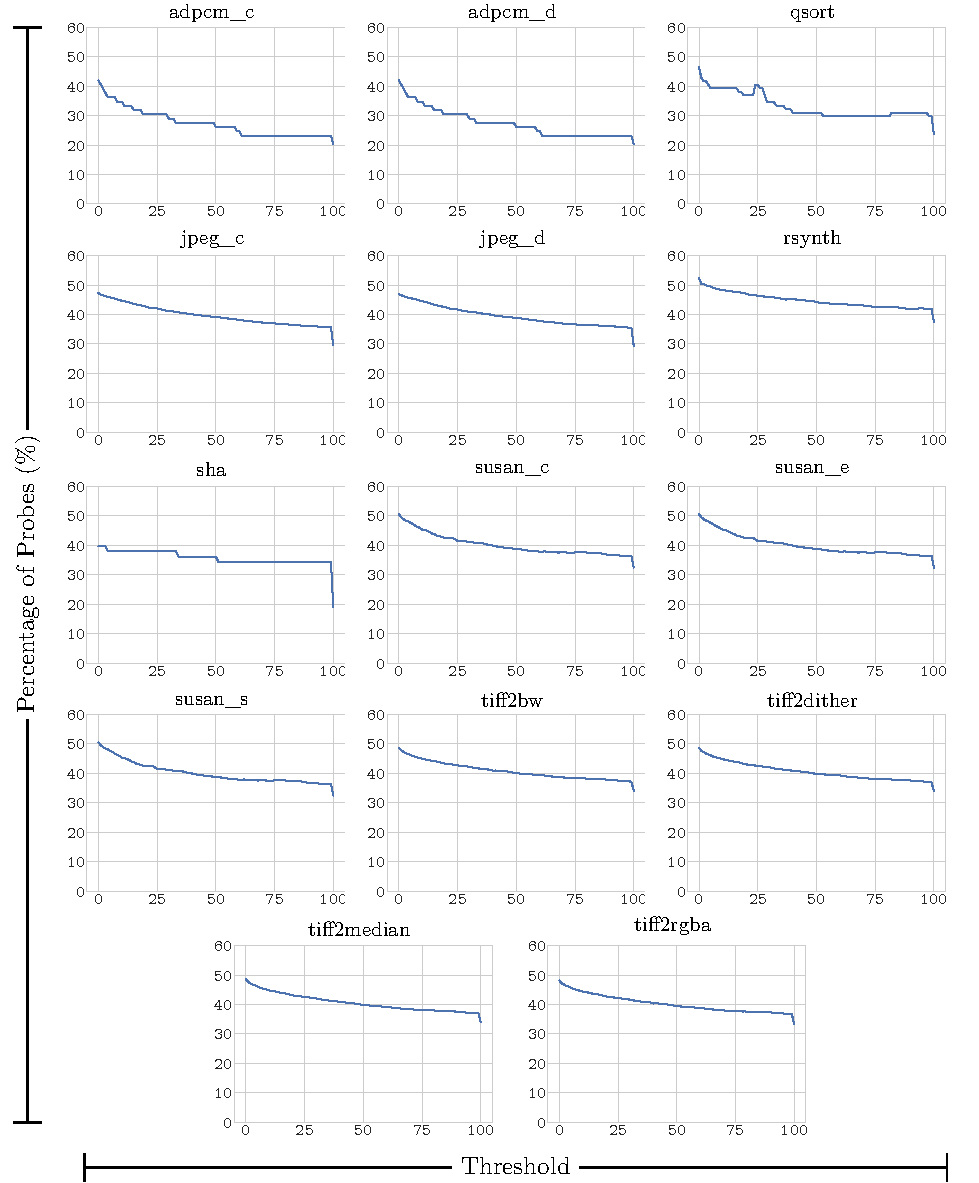
\includegraphics[width=\textwidth]{figs/instr-all-thresholds.pdf}
    \caption{Percentage of instrumented basic blocks, relative to the optimal profiling, for both relaxation algorithms when varying the threshold from 0\% up to 100\%.}
    \label{fig:instr-all-thresholds}
\end{figure}

In order to investigate the effects caused to the instrumentation when varying the relaxation threshold for both relaxation algorithms, we performed a full analysis of the reduction in the number of probes varying the threshold from 0\% up to 100\%, as presented in Figure~\ref{fig:instr-all-thresholds}.
This figure shows the percentage of instrumented probes relative to the optimal profiling.
It is interesting to understand some of the aspects of these results.
In some cases, when increasing the threshold, the number of probes also increased, e.g., as it is noticeable in the {\flagstype qsort} benchmark.
This happens when the larger threshold allows the 0-1 knapsack solver to exchange a large number probes for fewer probes with higher execution frequency and also higher error.
It is also interesting to notice the highly conservative aspect of the relaxation algorithm that operates per DAG, as all benchmarks remain with more than 40\% of the same probes as the optimal profiling, even with a relaxation threshold of 100\%.
This happens as the static error is computed based on the path with the minimum amount of work possible in the DAG, which can be very conservative in most cases.

On the other hand, the whole program relaxation can significantly reduce the number of probes.
This is possible for two main reasons: first, there are several probes which are never executed, as shown in Figure~\ref{fig:null-probes-relative-to-optimal};
second, the WPO relaxation relies on profiling information from previous execution, which allows it to perform a more aggressive relaxation.

\subsection{Dynamic Evaluation}

For the evaluation of the performance overhead that the instrumentation incur to the benchmarks, we measure the wall-clock time of the benchmarks when compiled with the default {\flagstype -O3} optimisation.
For each benchmark, we compute the average overhead over all its 1000 input dataset.
When measuring the wall-clock time for each input, in order to reduce noise, we execute the same input until we have a statistically sound measurement, i.e. we execute until we have an interval no larger than 1\% with 99\% confidence.
Figure~\ref{fig:overhead-O3} shows the performance overhead imposed by the work instrumentation on the benchmarks when compared to their non-instrumented counterparts.
Figure~\ref{fig:overhead-improvement-O3} indicates the improvement of the relaxation algorithm over the optimal instrumentation, regarding the reduction in overhead.

\begin{figure}[ht]
    \centering
    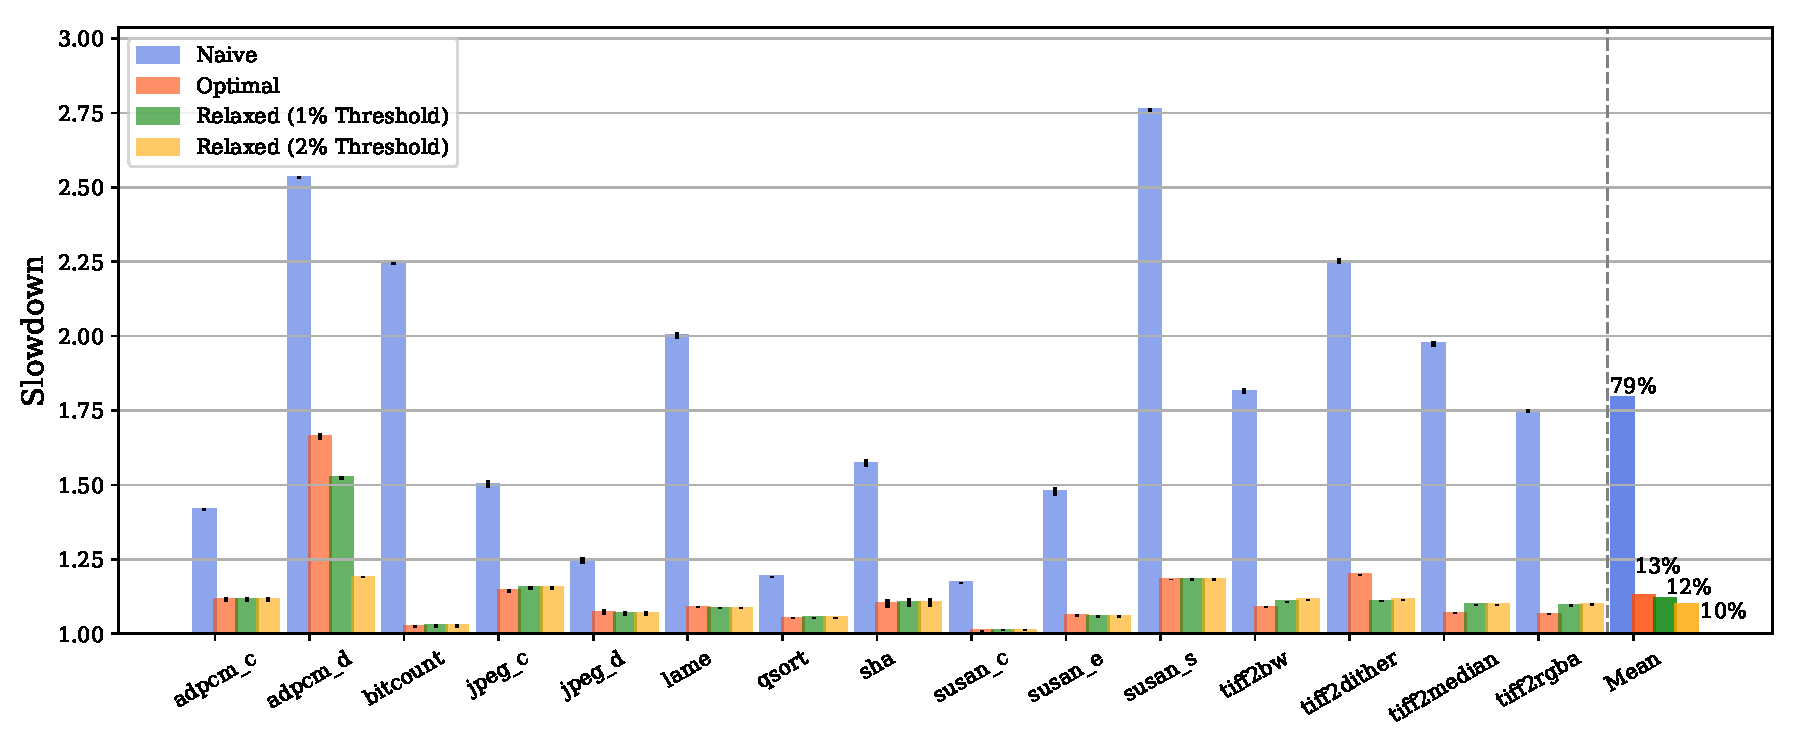
\includegraphics[width=\textwidth]{figs/overhead-O3.pdf}
    \caption{Overhead of the instrumentations compiled with {\flagstype -O3}.}
    \label{fig:overhead-O3}
\end{figure}

The WPO relaxation was performed using profiling information for every specific input, which provides the perfect information to perform the WPO relaxation.
This means that the experiments show its best performance enabled by having perfect profiling information.

\begin{figure}[ht]
    \centering
    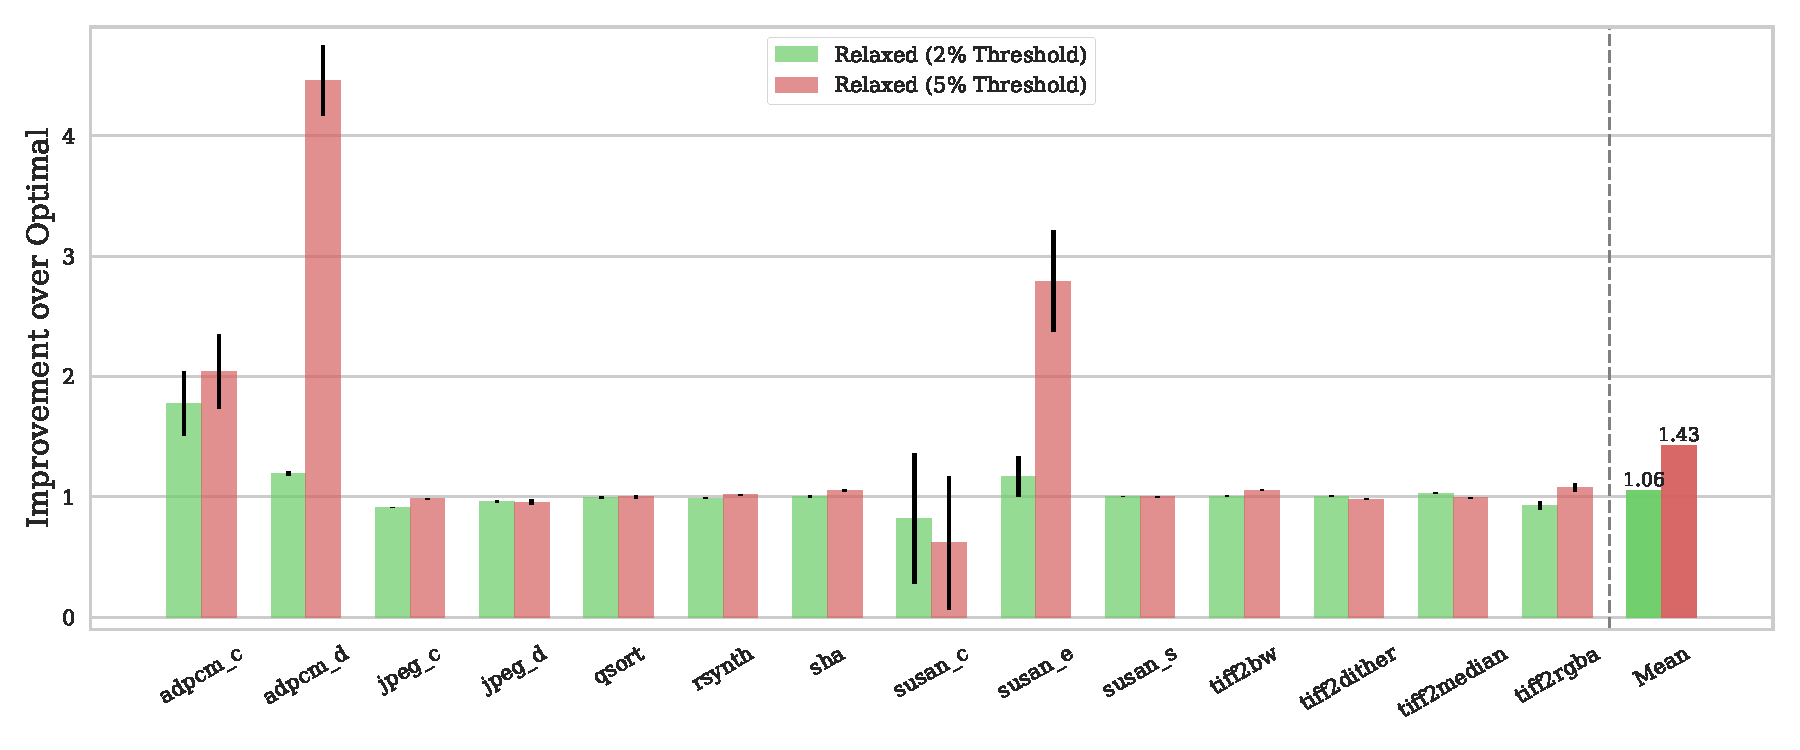
\includegraphics[width=\textwidth]{figs/overhead-improvement-O3.pdf}
    \caption{Overhead of the instrumentations compiled with {\flagstype -O3}.
             Notice that the average of the ratios does not equal the ratio of the averages.}
    \label{fig:overhead-improvement-O3}
\end{figure}

\begin{figure}[h!]
    \centering
    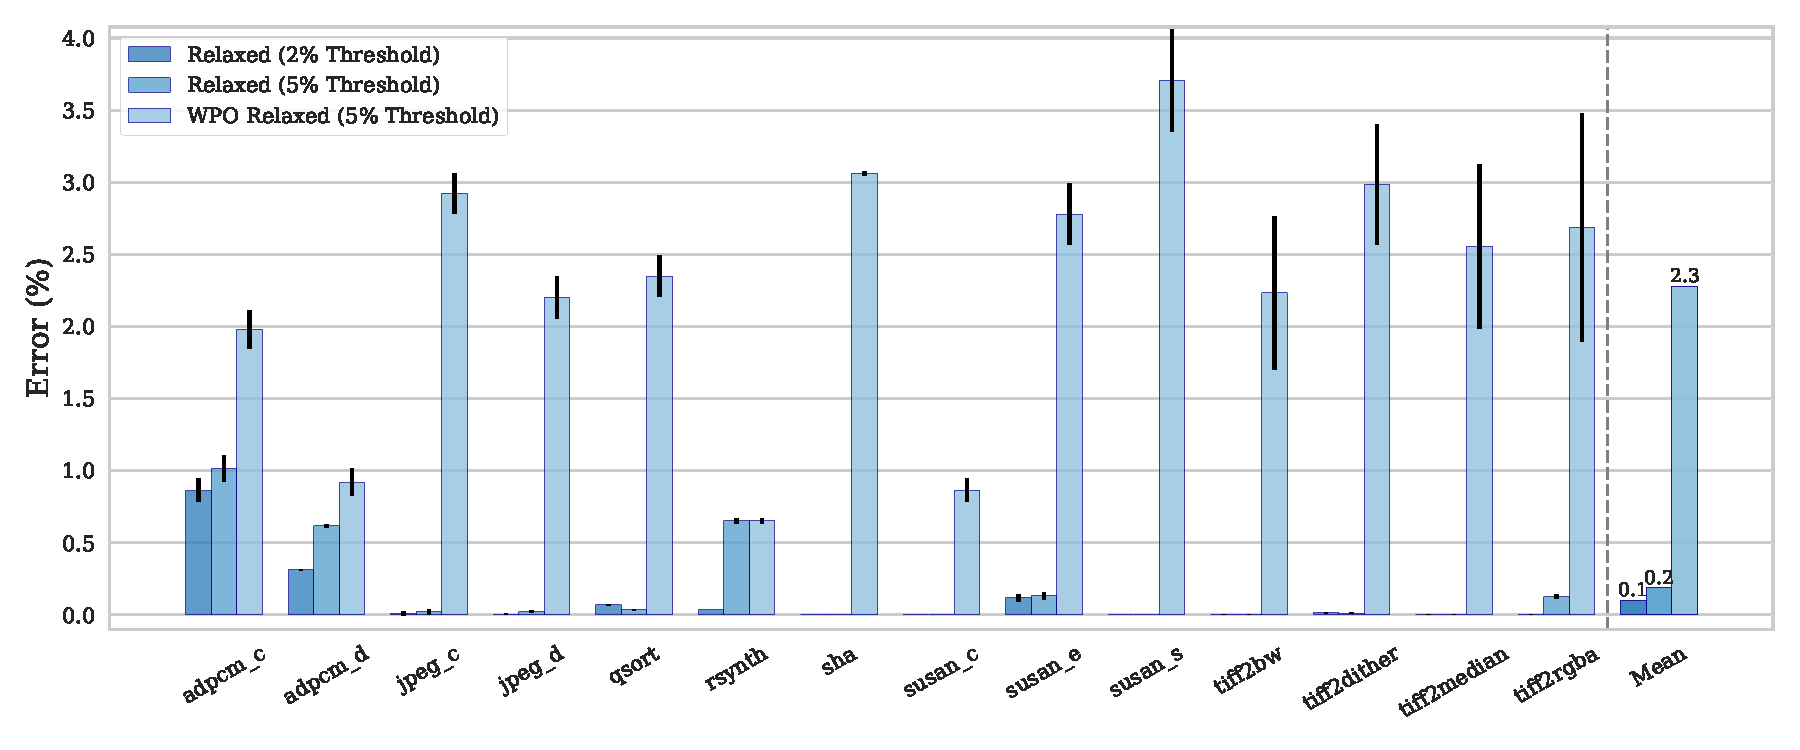
\includegraphics[width=\textwidth]{figs/error-O3.pdf}
    \caption{Dynamic error of the work profiling averaged over the 1000 inputs, after relaxing the number of probes.}
    \label{fig:error-O3}
\end{figure}

Figure~\ref{fig:overhead-improvement-O3} shows that the relaxation algorithm, with 5\% threshold, is able to improve an average of 48\% over the optimal instrumentation, 
and the WPO relaxation achieves an average of $2\times$ improvement over the optimal instrumentation.
While the optimal profiling has a maximum overhead of almost 60\%, the work profiling with a relaxation of 5\% threshold has an overhead of less than 20\% for all benchmarks,
with the WPO relaxation reaching an average overhead of only 5\%, compared to an average of 12\% for the optimal profiling.

%improving about $4.5\times$ for both the {\flagstype adpcm\_d} and {\flagstype susan\_e} benchmarks.
%If we disconsider the exceptional improvement for the \texttt{adpcm\_d} benchmark, the relaxation algorithm with a 5\% threshold is able to improve an average of about 20\% over the optimal instrumentation.
Furthermore, these improvements can be obtained while incurring very little dynamic error, as shown in Figure~\ref{fig:error-O3}.
This result confirms the overly conservative aspect of the relaxation algorithm applied per DAG,
while the WPO relaxation is significantly less conservative.
Because we performed the WPO relaxation having perfect profiling information, its dynamic error was always below the 5\% thresholds.
Although it is not guaranteed by the algorithm, profiling representative inputs should also result in small dynamic errors.


%\textbf{Profile-guided Instrumentation.}

%\textbf{Code size.}
%\begin{figure}[ht]
%    \centering
%    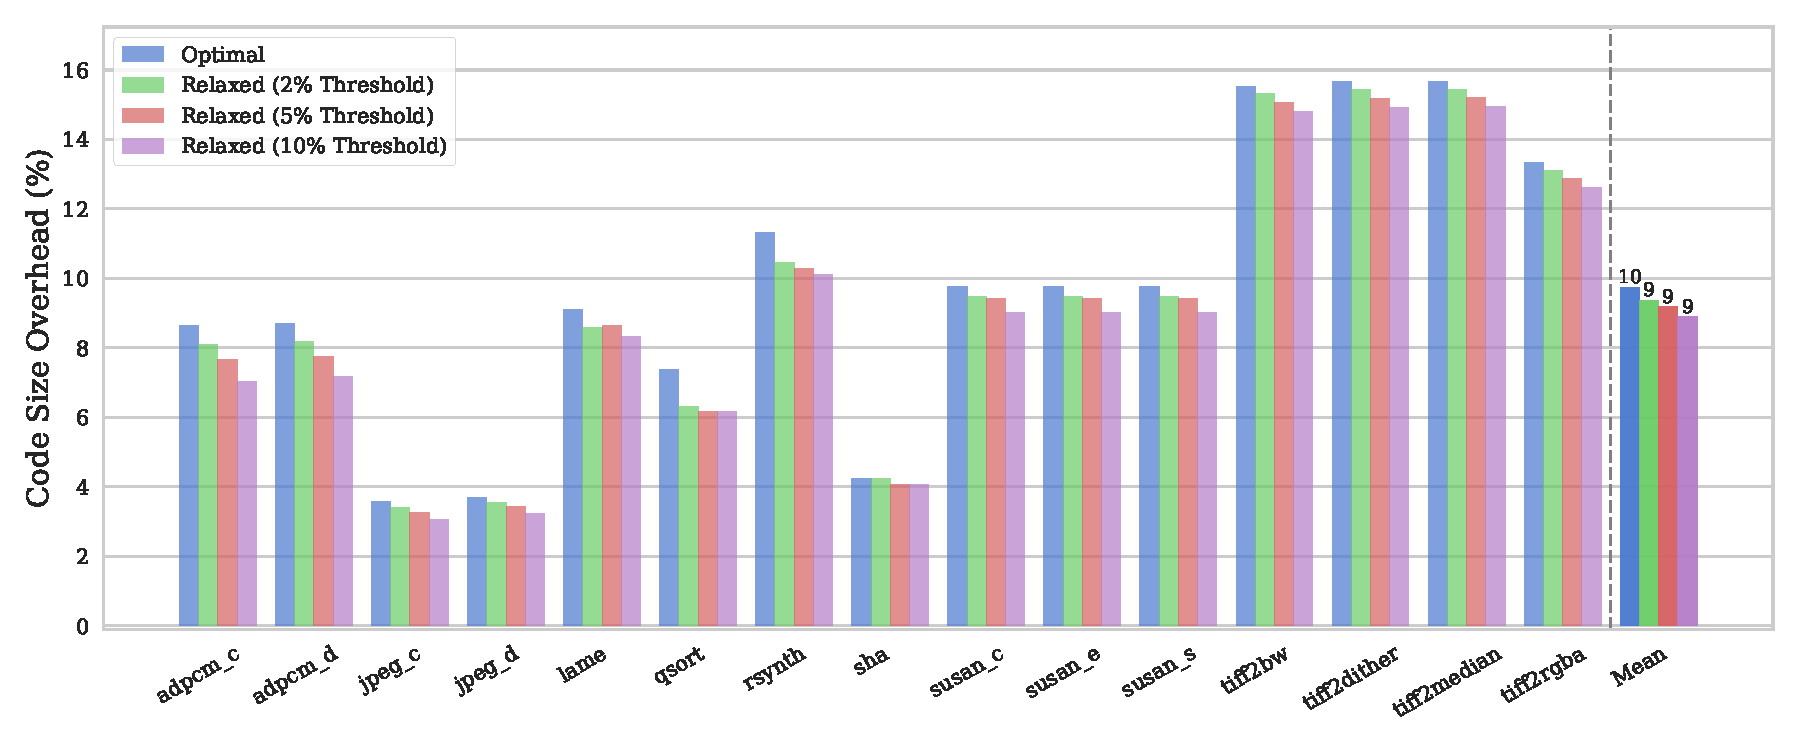
\includegraphics[width=\textwidth]{figs/code-size-probes.pdf}
%    \caption{Percentage of instrumented basic blocks for the optimal and the relaxed instrumentation with different relaxation thresholds.}
%    \label{fig:num-probes}
%\end{figure}
%
%\begin{figure}[ht]
%    \centering
%    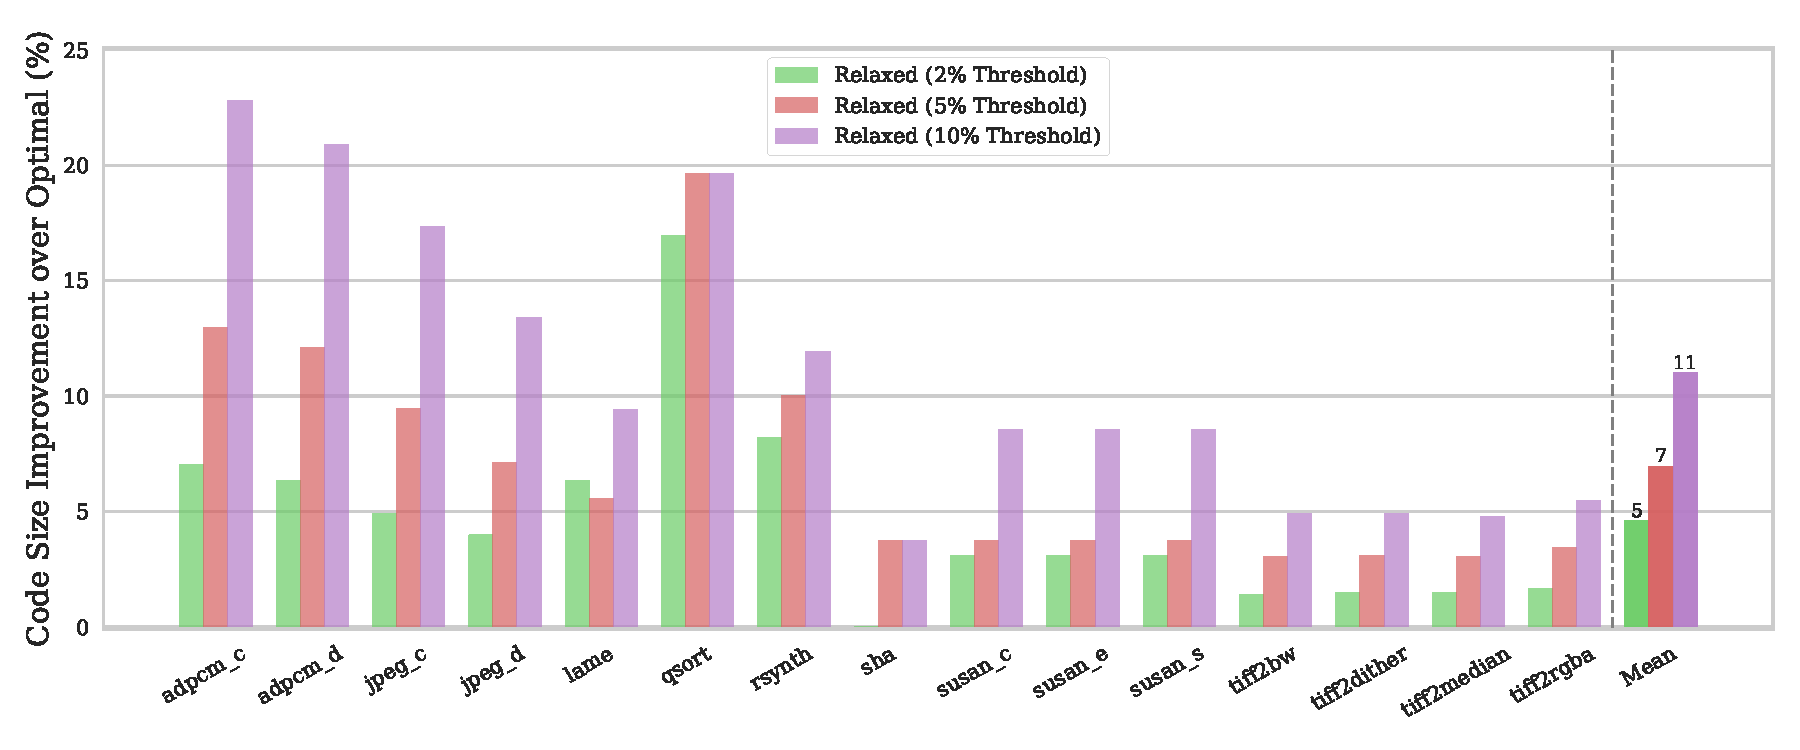
\includegraphics[width=\textwidth]{figs/code-size-probes-improvement.pdf}
%    \caption{Percentage of instrumented basic blocks for the optimal and the relaxed instrumentation with different relaxation thresholds.}
%    \label{fig:num-probes-improvement}
%\end{figure}


%In this section we discuss the three baseline implementations that will be used for assessing the quality of the proposed metric.

%\vspace{1ex}
%\noindent \textbf{{\Itercomp} over a single input}

%Most of the existing {\itercomp} studies find the best optimisation though repeated runs on the same input.
%Although this approach will usually lead to sub-optimal performance across large input datasets, it provides a good baseline when considering the complexity and resonably low compile-time regarding iterative optimising compilers.
%If $M$ is the total number of combinations of compiler optimisations, this approach requires $O(M)$ runs of the program being optimised.
%We can consider two main scenarios:
%\textit{($i$ - best case scenario)} after selecting the optimisation over each individual input, consider the one with best performance across the whole input dataset;
%\textit{($ii$ - expected scenario)} after selecting the optimisation over each individual input, consider the average case of their performance across the whole input dataset.

%\vspace{1ex}
%\noindent \textbf{{\Itercomp} across large input datasets}

%Recent work on {\itercomp} have been targeting optimisation across multiple inputs~\cite{fursin07,chen10,chen12a}.
%If $N$ is the number of input test cases and $M$ is the total number of combinations of compiler optimisations, they perform a total of $O(NM)$ runs of the program being optimised.
%Similarly to what have been discussed previously, there are different ways for how to determine the optimal combination of compiler optimisations across multiple inputs.
%It is possible to tune the selection of the program-optimal combination to minimise risk or to maximise average performance.
%A compromise-based selection criterion could be to maximise average speedup with minimised variance.
\newpage
\subsection{Case Studies}

\noindent \textbf{Analysis of the Best Improvement in Overhead: {\flagstype adpcm\_d}}

\begin{figure*}[htb]
    \centering
    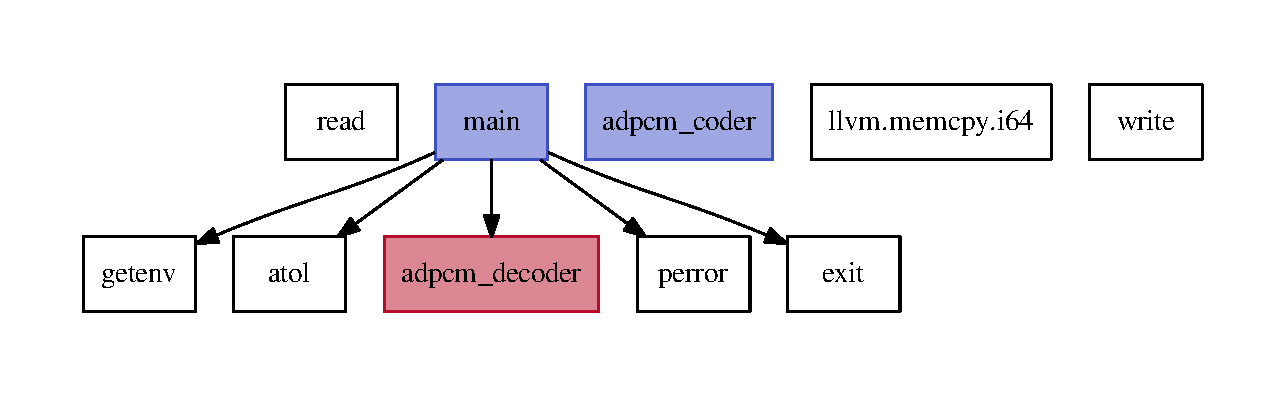
\includegraphics[width=0.9\textwidth]{figs/adpcm_d-heat-callgraph.pdf}
    \caption{Call graph highlighting the maximum basic block frequency of each function, using a cool/warm colour map.}
    \label{fig:adpcm_d-heat-callgraph}
\end{figure*}

The {\flagstype adpcm\_d} benchmark is the most critical case amongst the evaluated benchmarks, with an overhead of about 59\% for the optimal instrumentation.
Figure~\ref{fig:adpcm_d-heat-callgraph} shows the \textit{heat} call-graph of the {\flagstype adpcm\_d} benchmark, with each function coloured based on their maximum basic block frequency, using a cool/warm colour map.
This benchmark has a single hot function, namely the function called \verb|adpcm_decoder|.
Moreover, it consists mainly of a single hot loop with several branches inside it, as depicted by Figure~\ref{fig:adpcm_d-cfg-instr}.
The relaxation algorithm is able to reduce this overhead down to about 47\% (with a static error threshold of 2\%) and 14\% (with a static error threshold of 5\%) by removing only one and two probes from the hot loop, respectively.
These overhead reductions represent a 20\% and 4.5$\times$ improvement over the optimal algorithm, with 2\% and 5\% relaxation threshold respectively.
The two relaxed probes were placed in branches, inside the hot loop, with a high probability of being taken, but with a small contribution to the total amount of work measured in the loop.

\begin{figure}[H]
    \centering
    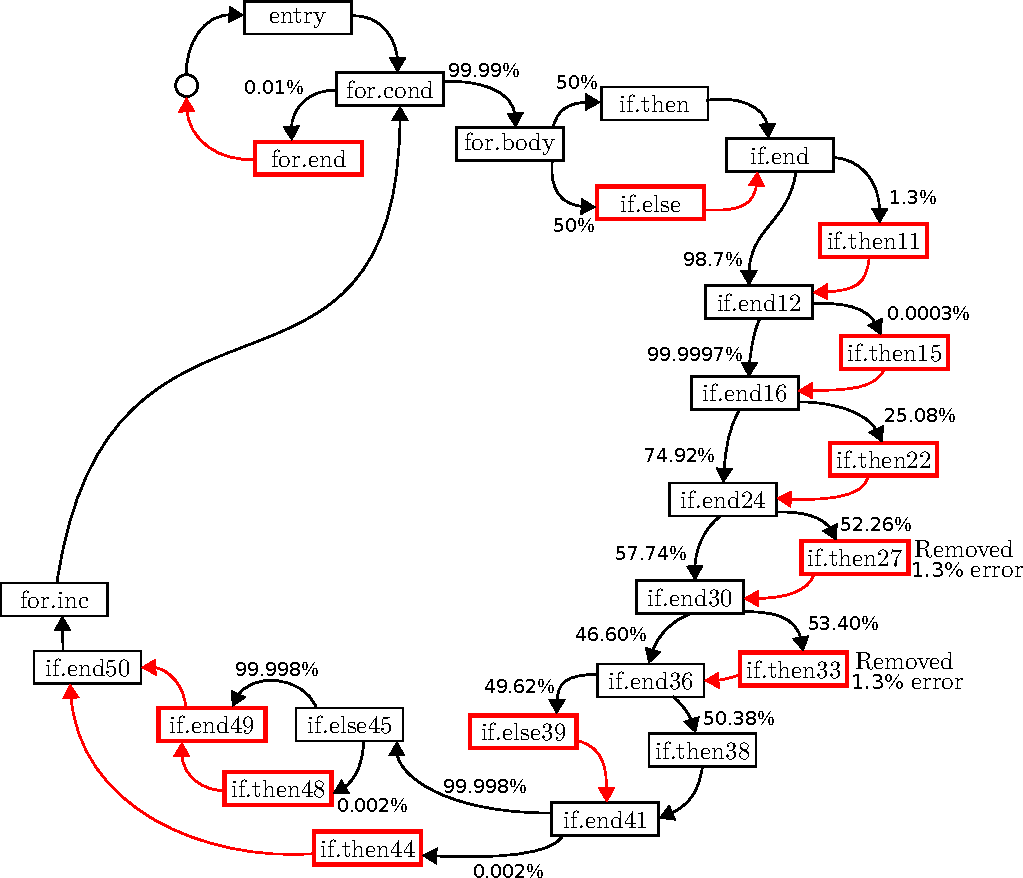
\includegraphics[width=0.8\textwidth]{figs/adpcm_d-cfg-instr.pdf}
    \caption{CFG of the function that contains the hot loop of the {\flagstype adpcm\_d} benchmark.}
    \label{fig:adpcm_d-cfg-instr}
\end{figure}

Figure~\ref{fig:adpcm_d-probes-err-freq} shows all the probes necessary for the function that contains the hot loop of the {\flagstype adpcm\_d} benchmark.
Notice that the relaxation was able to remove all probes with a static error lower than the 5\% threshold.
Because these probes were placed in basic blocks with a considerable execution frequency, their removal resulted in a significant reduction in performance overhead.

\begin{figure}[H]
    \centering
    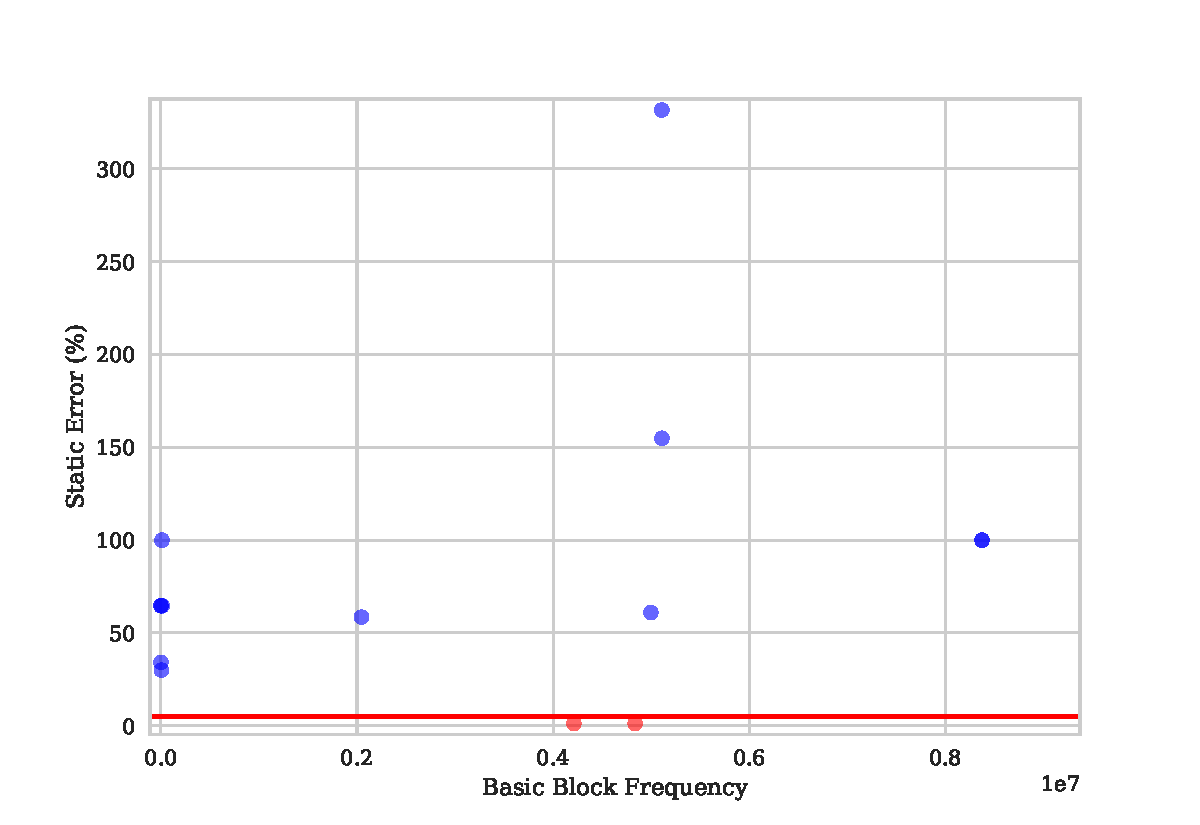
\includegraphics[width=0.8\textwidth]{figs/adpcm_d.pdf}
    \caption{Comparison between probe frequency and static error for the {\flagstype adpcm\_d} benchmark. The red line marks the 5\% threshold limit.}
    \label{fig:adpcm_d-probes-err-freq}
\end{figure}

\noindent \textbf{Analysis of the Abnormal Regression: {\flagstype susan\_c}}

The {\flagstype susan\_c} presents an abnormal regression as relaxation seems to increase the profiling overhead.
This increase in profiling overhead is counter-intuitive because the relaxation algorithms are able to reduce the number of instrumented probes.
Although we could not pinpoint the precise reason for this abnormal regression, we can provide an analysis of this benchmark.

Figure~\ref{fig:susan_c-probes-err-freq} shows that most probes are rarely or never executed, in accordance with Figure~\ref{fig:null-probes-relative-to-optimal},
with only a few probes being highly executed, and some of these frequently executed probes were not removed by the relaxation algorithm.

Another important aspect to point out is the difference among the final CFGs after applying the {\flagstype -O3} optimisation.
Although relaxation does not directly alter the CFG, it is important to notice that many optimisation passes make use of LLVM's built-in target-based cost model,
which means that adding or removing instructions from basic blocks may affect decisions during transformations of the code.
For example, there are optimisations for loop-unrolling, function inlining, and simplifications of the CFG, that make use of this built-in cost model.
Although this difference in the CFGs may not be the only reason for the increase in overhead, it is one of the reasons, since changes in the CFG may affect other compiler and hardware optimisations, such as instruction caching.

\begin{figure}[H]
    \centering
    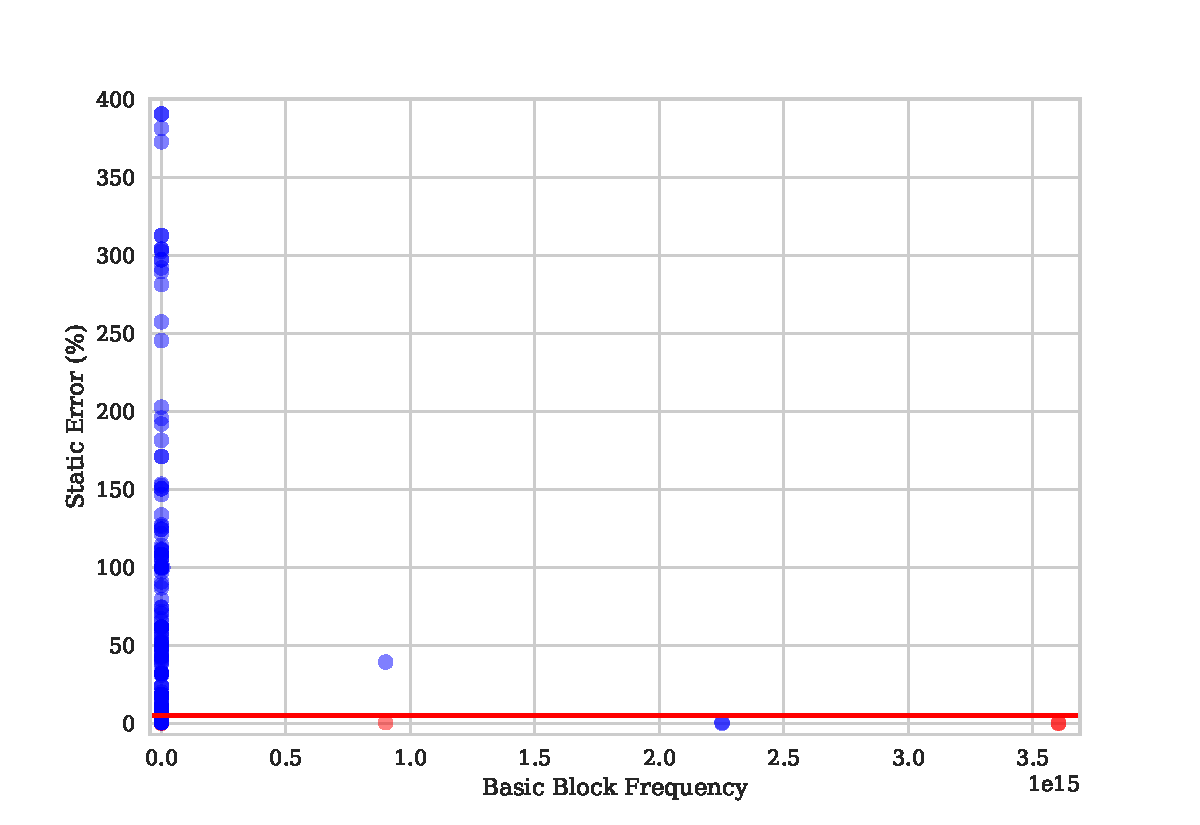
\includegraphics[width=0.8\textwidth]{figs/susan_c.pdf}
    \caption{Comparison between probe frequency and static error for the {\flagstype susan\_c} benchmark. The red line marks the 5\% threshold limit.}
    \label{fig:susan_c-probes-err-freq}
\end{figure}

%\vspace{1ex}
%\noindent \textbf{{\Itercomp} based on the IPC metric}

%While the previous two baselines addresses two opposite aspects of {\itercomp}, namely, compile-time efficiency and performance of the generated code, we also intend to compare against IPC as the competing baseline.
%The main reason for comparing against IPC is because it has been proposed as a metric for comparing the performance of two optimisations running on two distinct inputs.
%If $M$ is the total number of combinations of compiler optimisations, this approach requires $O(M)$ runs of the program being optimised.

\section{Evaluation of the Online {\IterComp}}

In this section, we evaluate the online {\itercomp} guided by the WP metric.
For comparison, we use four configurations\footnote{A configuration using the WPO relaxation was not used due to the time necessary for executing the experiments.}.
In all configurations, the same optimisation sequence is used for multiple inputs, using a dynamic input-window size, as explained in Section~\ref{sec:oic-infra}.
The average performance over the input window provides an estimate for the overall performance of the optimisation sequence across distinct inputs.
The optimisation sequences are ranked based on their average performance, and the best optimisation sequence is selected.
%When selecting the best optimisation sequence, they are ranked by the average of their performance measurement, using the WP metric, except for the Oracle-RM which uses the real speedup over \texttt{-O0}.
\begin{itemize}
\item \textbf{Oracle-RM} executes the program multiple times for each input, measuring the real speedup for each optimisation sequence, and then uses the real speedup over {\flagstype -O0} for comparing the optimisation sequences.
  The speedups are computed based on the wall-clock time.
  In order to reduce noise, the program is executed several times for the same input, until the confidence interval was no larger than 1\% for a 99\% confidence.
\newpage
\item \textbf{Oracle-PP} represents an oracle with a \textit{perfect} non-intrusive profiling.
  Although it uses the WP metric for comparing optimisation sequences, this oracle also avoids noise in its measurements by also executing the program multiple times for each input.
  The first execution is used for profiling the work metric.
  The remaining executions are used for measuring the wall-clock time without using the work profiling.
\item \textbf{Real-OP} corresponds to the online {\itercomp} as it would be applied in a real online scenario.
  For each optimisation, a random sample of inputs is selected, and the program is executed only once with each input.
  When executing each input, it uses the optimal work instrumentation for profiling the work metric.
  The average of the WP for the sample of inputs is then used for selecting the best optimisation.
\item \textbf{Real-R5} is similar to the {Real-OP}.
  It also corresponds to the online {\itercomp} as it would be applied in a real online scenario.
  For each optimisation, a random sample of inputs is selected, and the program is executed only once with each input.
  When executing each input, it uses the relaxed work instrumentation, with a 5\% threshold, for profiling the work metric.
  The average of the WP for the sample of inputs is then used for selecting the best optimisation.
\item \textbf{Real-IPC} corresponds to the online {\itercomp} based on the IPC metric.
  For each optimisation, a random sample of inputs is selected, and the program is executed only once with each input.
  The average of the IPC metric for the sample of inputs is then used for selecting the best optimisation.
\end{itemize}
The comparison between Oracle-RM and Oracle-PP is useful for validating the use of the WP metric for guiding {\itercomp}, while the other configurations demonstrate the viability of applying the online {\itercomp} in a real scenario.

Figure~\ref{fig:window-size} shows the average input-window size for each benchmark and configuration.
It shows that we can have a statistically sound measurement of the performance metric using just a small number of inputs.

\begin{figure}[htb]
    \centering
    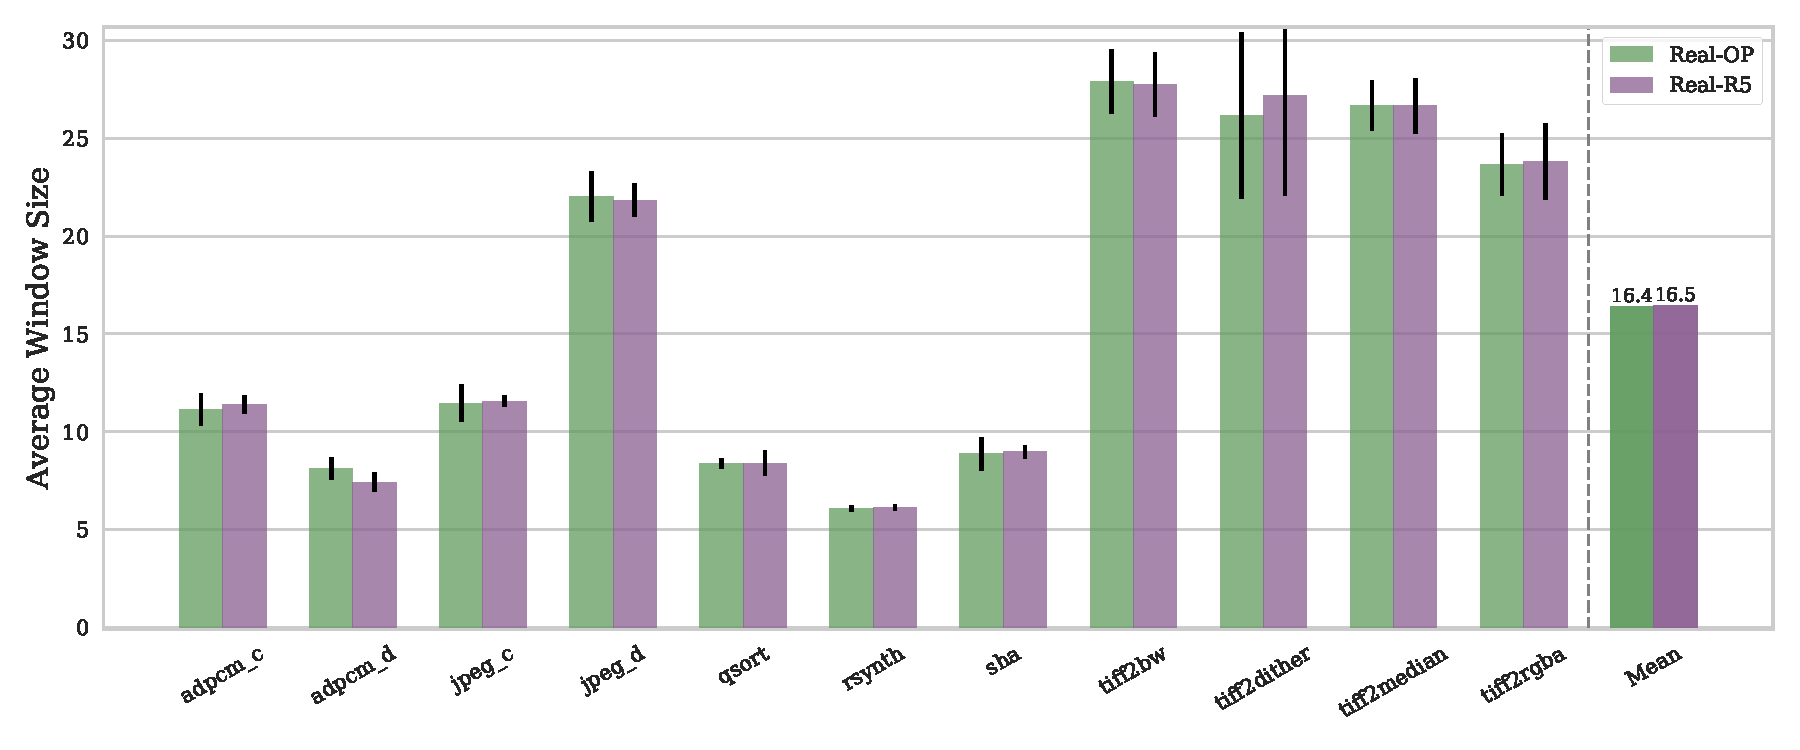
\includegraphics[width=\textwidth]{figs/window-size.pdf}
    \caption{Average input-window sizes observed during the online {\itercomp}.}
    \label{fig:window-size}
\end{figure}
\newpage
\subsection{The Set of Optimisation Sequences}

For the purpose of evaluating the use of the WP metric with {\itercomp}, we collected in advance a fixed set of optimisation sequences.
The reason for using this fixed set, as explained in Section~\ref{sec:oic-infra}, is because this thesis is focused on other components of the infrastructure for performing {\itercomp} and we assume that a good generator of optimisation sequences will be used in a real online scenario.
This set contains 500 optimisation sequences collected in a random search using the training benchmarks.
These optimisation sequences contain an average of 40 individual optimisation passes, including repetitions, with a maximum of 119 optimisation passes, but it also contains optimisation sequences which consist of a single flag, such as the default optimisations {\flagstype -O1}, {\flagstype -O2}, {\flagstype -O3}, {\flagstype -Os}, and {\flagstype -Oz}.

  \begin{minipage}{0.9\textwidth}
     \vspace{1em}
     \singlespace
     \noindent\textbf{Example of a short optimisation sequence:}\vspace{-1ex}
     \justify{\flagstype -mem2reg -simplifycfg -constprop -dce}
  \end{minipage}

  \begin{minipage}{0.9\textwidth}
     \vspace{1em}
     \singlespace
     \noindent\textbf{Example of a long optimisation sequence:}\vspace{-1ex}
     \justify{\flagstype -globalopt -reassociate -instcombine -loop-rotate -block-freq -deadargelim -early-cse -sroa -argpromotion -sccp -tbaa -barrier -constmerge \mbox{-loop-vectorize} -domtree -basicaa -memdep -basiccg -memcpyopt \mbox{-constprop} -adce -globaldce -mem2reg -constmerge \mbox{-globaldce} -constprop -instsimplify -dse -dce -simplifycfg -loop-unroll -reassociate -constprop \mbox{-globaldce} -instsimplify -adce -constmerge -bb-vectorize -dce -mergefunc -simplifycfg -dse -loop-unroll -globaldce}
  \end{minipage}

  \begin{minipage}{0.9\textwidth}
     \vspace{1em}
     \singlespace
     \noindent\textbf{Example of an optimisation sequence which includes {-O3}:}\vspace{-1ex}
     \justify{\flagstype -O3 -adce -globaldce -simplifycfg -memcpyopt -reassociate -mergefunc \mbox{-dce} -dse}
     \vspace{2em}
  \end{minipage}

Repeating the same optimisation pass can be beneficial and usually expected by other passes.
For example, the {\flagstype -loop-simplify} pass is used for transforming loops into a canonical form by inserting pre-header and exit basic blocks.
Although this pass inserts jumps due to redundant basic blocks, this canonical form can be favourable to other loop optimisations.
Because of the redundant basic blocks, this optimisation pass expects that the {\flagstype -simplifycfg} will eventually be executor later on the optimisation pipeline.
Another example of such inter-relation between transformations concerns the {\flagstype -licm} and {\flagstype -mem2reg} passes.
The {\flagstype -licm} pass is responsible for moving invariant code out from the loop body.
It usually creates new local variables, using memory access operations, for assisting with the code manipulation, which means that the executing the {\flagstype -mem2reg} pass afterwards would be useful as a cleanup pass for removing the extra memory accesses generated.
However, many of the analysis required for identifying loop invariant also benefit from the transformations performed by the {\flagstype -mem2reg} pass.
These examples illustrate the importance of repeating optimisation passes.
Moreover, they illustrate the intricate relation amongst several transformations.

However, all optimisation sequences in the set of optimisations were generated completely at random, without using any knowledge of individual transformations.
Each optimisation sequence was generated in two steps: \textit{(1)} randomly selects the number of flags; \textit{(2)} randomly selects the flags, allowing repetitions.
Afterwards, this randomly generated optimisation sequence would be included in the set of optimisation sequences only if it was able to improve the performance of a training benchmark, also selected at random, in respect of the {\flagstype -O3} default optimisation.
This process was repeated until we obtained all the 500 distinct optimisation sequences.

\subsection{Performance Evaluation}

In order to evaluate the quality of the final optimisation sequences selected by the {\itercomp} search, we compare their speedup by measuring wall-clock time of the benchmarks when compiled with the standard {\flagstype -O3} optimisation.
For each benchmark, after selecting the final optimisation sequence, we compute the average speedup over all the 1000 input dataset.
When measuring the wall-clock time for each input, to reduce noise, we execute the same input until we have a statistically sound measurement, i.e. we execute until we have an interval no larger than 1\% with 99\% confidence.
Figure~\ref{fig:speedups} shows these average speedups over all the 1000 input dataset.
This figure shows that the best optimisation sequence selected with the Oracle-PP is very close to the performance of the best optimisation sequence selected with the Oracle-RM.
This result is important for demonstrating that a work-based metric has the potential to produce good results in a real online scenario, where there is the restriction that programs execute distinct inputs only once.
Moreover, the evaluation also indicates that the use of relaxation algorithms does not degrade the optimisation search,
it might even benefit the {\itercomp} as it tends to insert smaller interferences in the performance measurement.
Finally, Figure~\ref{fig:speedups} also presents the results of {\itercomp} guided by IPC, which is futher discussed in Figure~\ref{fig:ipc-vs-work}.

\begin{figure*}[htb]
    \centering
    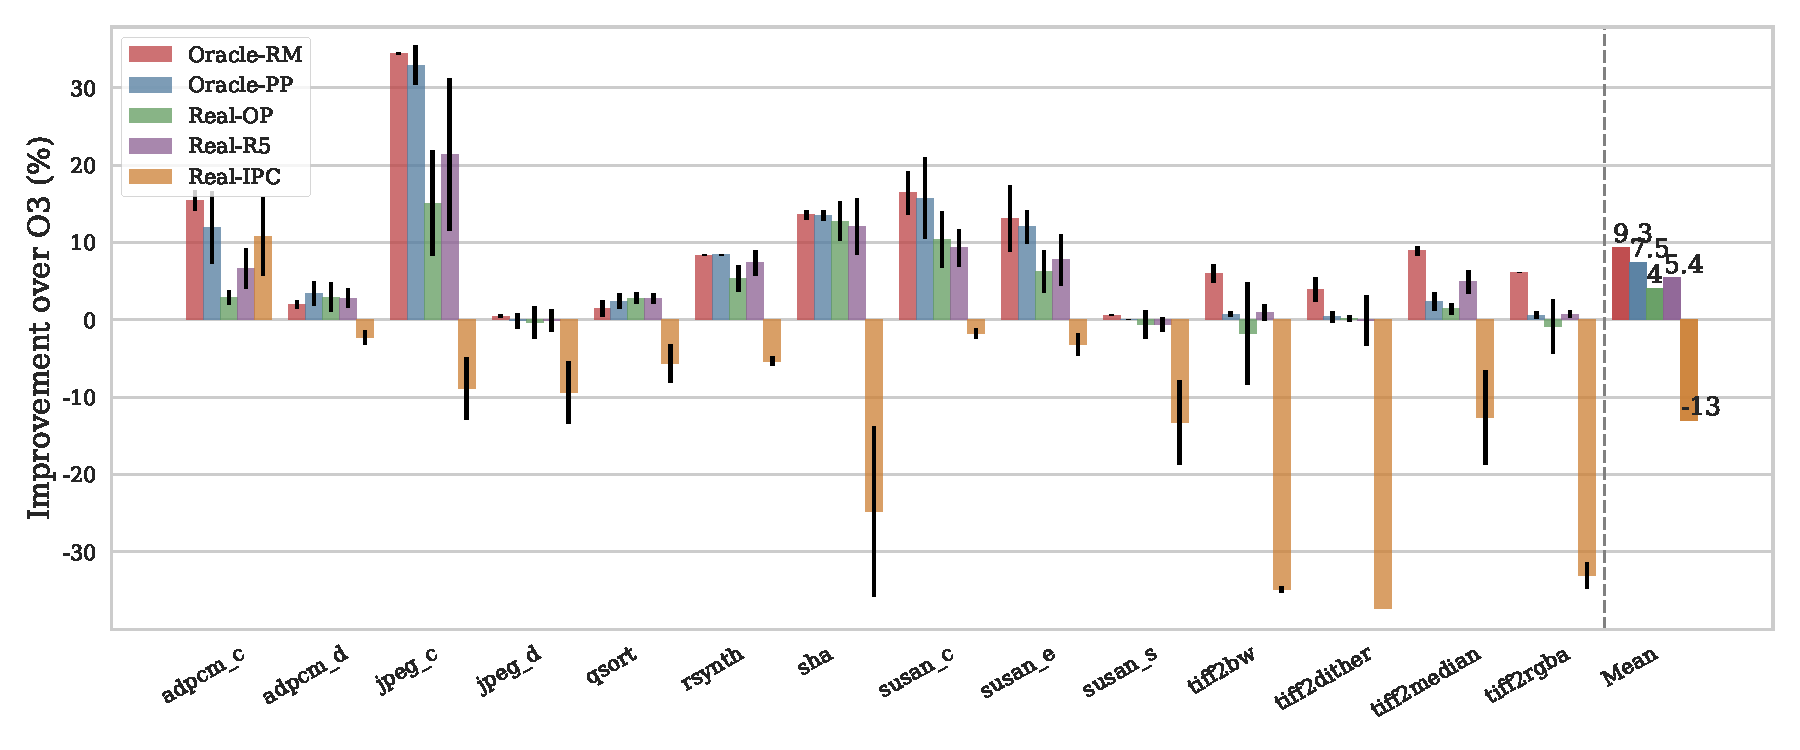
\includegraphics[width=\textwidth]{figs/speedups.pdf}
    \caption{Speedups obtained from the final optimisation sequence selected by the online {\itercomp}.
	         The speedups reported for each benchmark represents the average speedup across their complete 1000 input datasets.}
    \label{fig:speedups}
\end{figure*}

%It illustrates the expected upper bound by the online {\itercomp}.

\begin{figure}[h!]
    \centering
    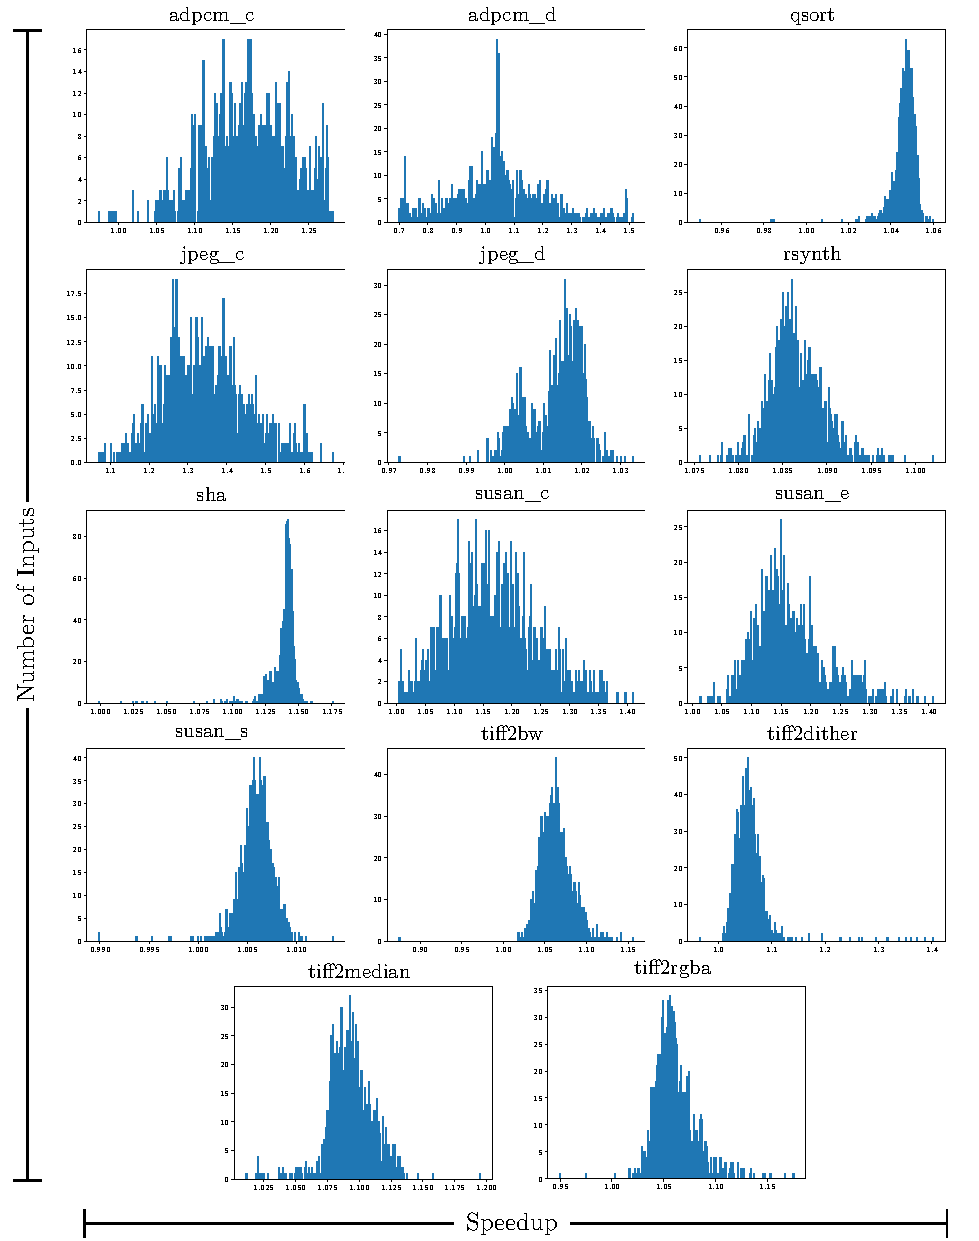
\includegraphics[width=\textwidth]{figs/speedups-per-input.pdf}
    \caption{Histograms for the speedups over {\flagstype -O3} with the complete dataset of 1000 inputs for each benchmark.
             In each case, we are using the optimisation sequence with the best average speedup over {\flagstype -O3}.
             This figure shows how the performance for some of the benchmarks are highly sensitive to the input.}
    \label{fig:speedups-per-input}
\end{figure}

\begin{figure}[h!]
    \centering
    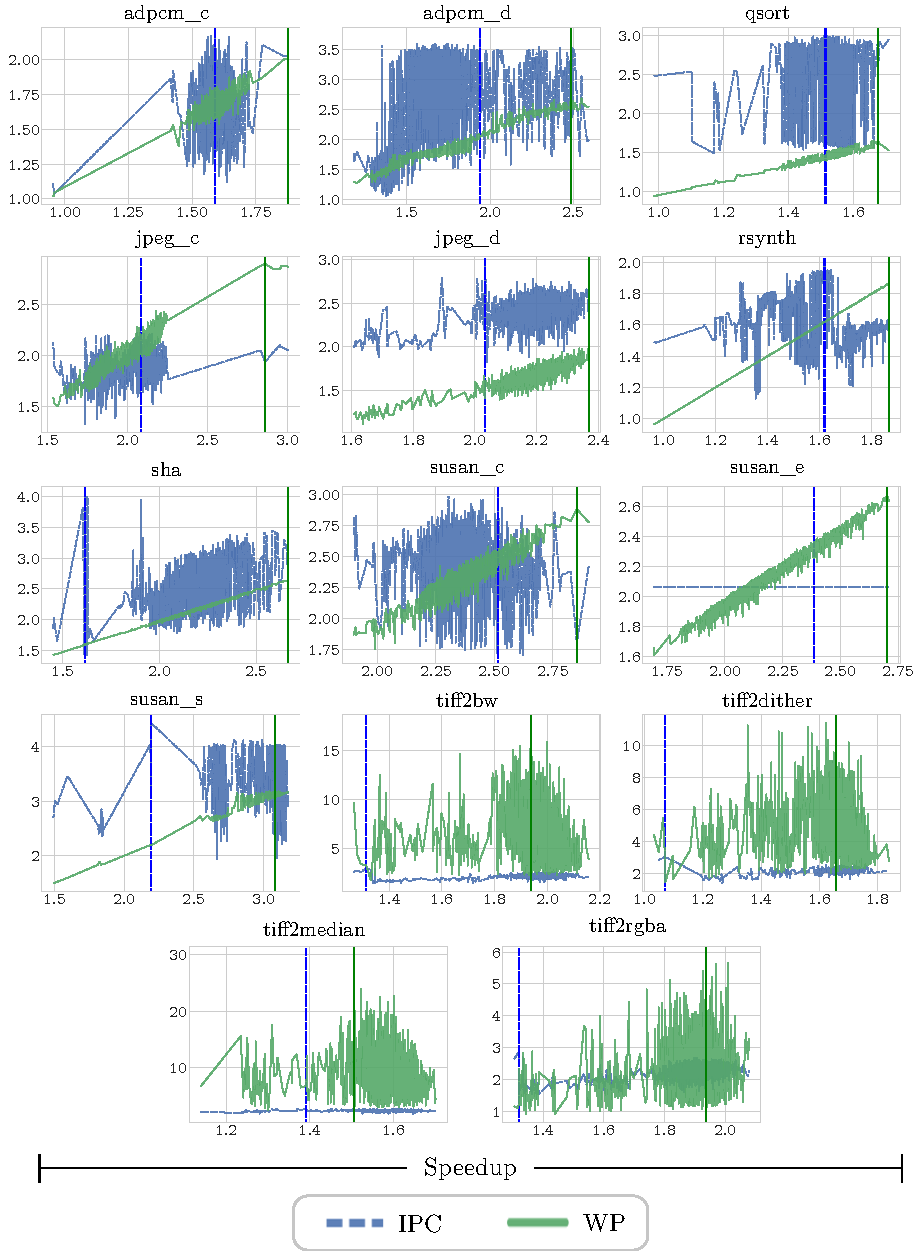
\includegraphics[width=\textwidth]{figs/ipc-vs-work.pdf}
    \caption{Comparison between {\itercomp} using IPC or the WP metric.}
    \label{fig:ipc-vs-work}
\end{figure}


Figure~\ref{fig:speedups-per-input} shows the histogram of the speedups obtained for each benchmark with all their respective 1000 inputs.
This figure shows the speedups of the best optimisation sequence found by the oracle with real measurements of execution time (Oracle-RM).
Figure~\ref{fig:speedups-per-input} is also important for showing that, although some of the benchmarks have a very consistent speedup for all their inputs,
other benchmarks are highly sensitive to the input.
For example, the optimisation sequence with best average performance for the {\flagstype jpeg\_c} benchmark presents a wide range of speedups across all its inputs,
varying from about 1 up to about 1.6 of speedup.
On the other hand, although the best optimisation sequence selected for the {\flagstype adpcm\_c} benchmark has a much shorter range of speedups, there is a clear concentration of inputs around different speedups.
These results corroborate the claim that performing {\itercomp} on a single input can be misleading and cause the optimisation search to overfit.

%\begin{figure*}[htb]
%    \centering
%    \includegraphics[width=\textwidth]{figs/profiled-speedups.pdf}
%    \caption{Speedups observed with the online {\itercomp} if we
%             consider the instrumentation overhead.}
%    \label{fig:profiled-speedups}
%\end{figure*}


Finally, Figure~\ref{fig:ipc-vs-work} presents a comparison between IPC and the WP metric regarding their correlation with the actual speedup over \verb|-O0| observed during {\itercomp}.
Each point in the figure corresponds to each metric averaged over input windows collected during multiple executions of the {\itercomp}.
The vertical lines correspond to the optimisation sequence selected by the {\itercomp} search, which either represents the highest IPC or the highest value of WP.
In all cases, the optimisation sequence selected based on the WP is much closer to the best speedup than the optimisation sequence selected based on IPC, which can be attributed to the fact that the WP has a stronger correlation with the speedup.
In all cases, IPC shows little to no correlation with the speedup, which corroborates the argument given in Section~\ref{sec:ipc-vs-work-metric}.

For some cases, namely for the tiff-related benchmarks, the WP shows a worse correlation with speedup.
We believe these cases could be improved by improving the cost model used to compute the work metric.
However, even in these cases, the optimisation sequences selected based on the WP outperform those selected based on the IPC metric.


% \subsection{Contribution of individual optimisation passes}
%
% Figure~\ref{fig:flagsfreq} shows an aggregated view of the final combination of compiler optimisations that were selected by {\itercomp} search.
% The figure presents the individual optimisation passes with at least 1\% of frequency in the selected combination of compiler optimisations that improved the performance over {\flagstype -O3}.
%
% \begin{figure*}[htb]
%     \centering
%     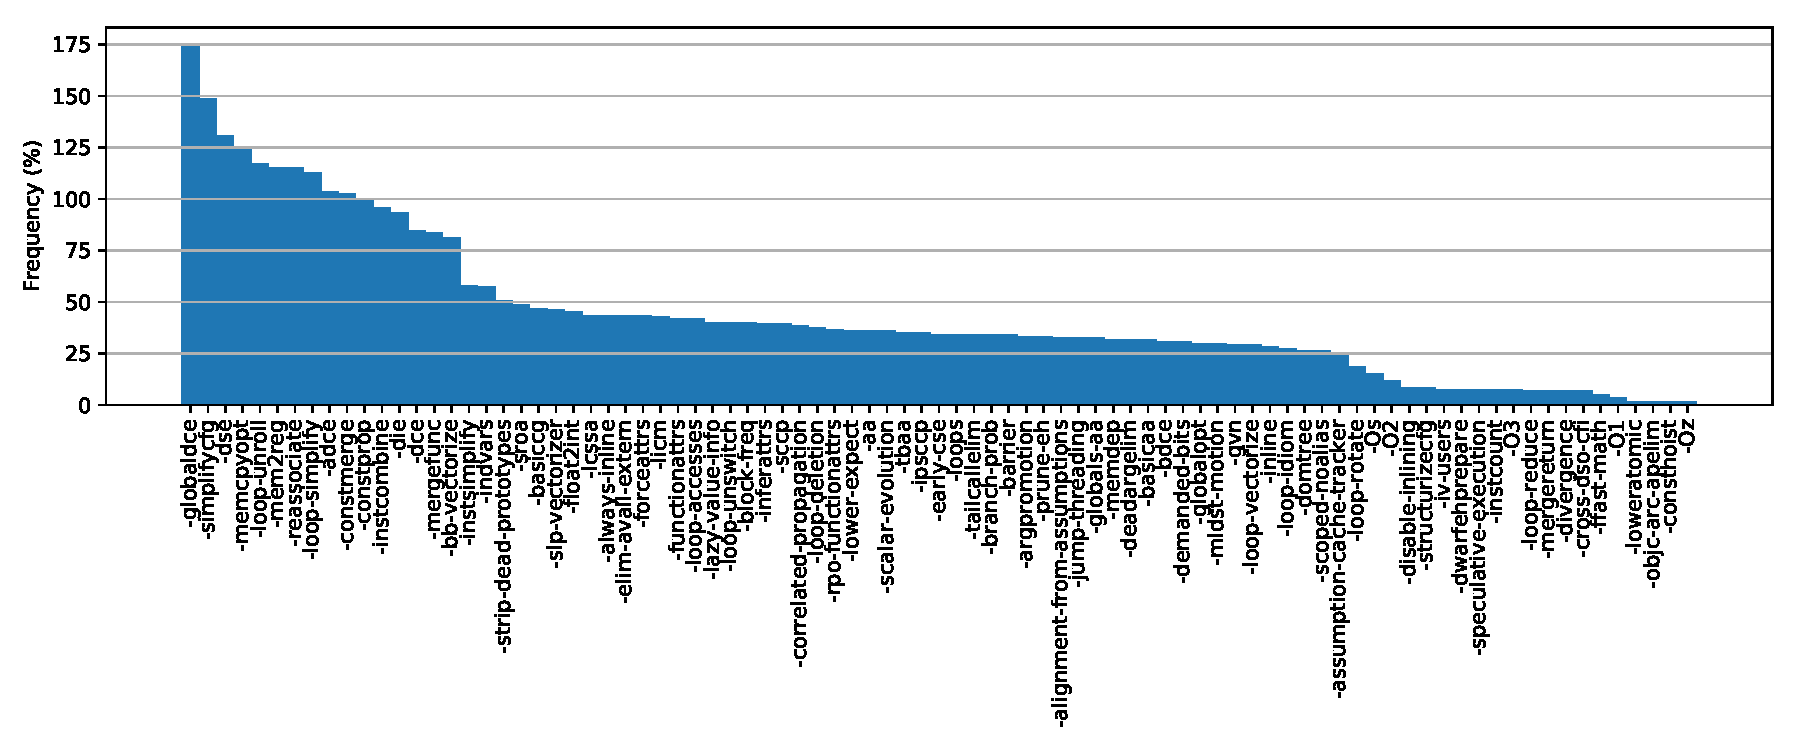
\includegraphics[width=\textwidth]{figs/flagsfreq.pdf}
%     \caption{Frequency of individual optimisation passes on the final selected
%              compiler optimisations of the {\itercomp} search over
%              all benchmarks.}
%     \label{fig:flagsfreq}
% \end{figure*}
%
% \subsubsection{Inter-Procedural Optimisations}
% %\begin{description}
% \noindent\textbf{Dead Global Elimination ({\flagstype -globaldce}):}
% It is an inter-procedural optimisation that eliminates unreachable internal globals from the program.
% It uses an aggressive algorithm that searches for global definitions that are known to be alive.
% After finding all live global definitions, it deletes all remaining globals.
% %This allows it to delete recursive chunks of the program which are unreachable.
%
% \noindent\textbf{Merge Functions ({\flagstype -mergefunc}):}
% This pass looks for equivalent functions that are mergable and folds them.
% It introduces a function encoding which allows it to provide a total-ordering for the function set.
% The total-ordering allows to arrange functions into the binary tree.
% When iterating over the functions, it checks for an equivalent function in tree.
% If an equivalent function exists, both functions are merged, otherwise, the new function is added to the tree.
% This pass focus mainly on improving code size and memory footprint.
% %The lookup routine has $O(log(n))$ complexity, while the whole merging process has complexity of $O(n\cdot log(n))$.
%
% \subsubsection{Transformations of the CFG}
%
% \noindent\textbf{Simplify the CFG ({\flagstype -simplifycfg}):}
% This optimisation simplifies the CFG by basic blocks merging and dead code elimination, such as:
% eliminates a basic block that only contains an unconditional branch;
% removes basic blocks with no predecessors;
% eliminates PHI nodes for basic blocks with a single predecessor; etc.
% This pass makes use of LLVM's built-in cost model to decide when it is beneficial for performing such transformations.
%
% \noindent\textbf{Canonicalise Natural Loops ({\flagstype -loop-simplify}):}
% This pass performs several transformations to convert natural loops into a simpler form, which makes subsequent analyses and transformations simpler and more effective.
% Loop pre-header insertion guarantees that there is a single, non-critical entry edge from outside of the loop to the loop header.
% This simplifies a number of analyses and transformations, such as Loop Invariant Code Motion (LICM).
% Loop exit-block insertion guarantees that all exit blocks from the loop (blocks which are outside of the loop that have predecessors inside of the loop) only have predecessors from inside of the loop (and are thus dominated by the loop header). This simplifies transformations such as store-sinking that are built into LICM.
% This pass also guarantees that loops will have exactly one backedge.
% Note that the {\flagstype -simplifycfg} pass will clean up blocks which are split out but end up being unnecessary, so usage of this pass should not pessimise generated code.
%
% \noindent\textbf{Unroll Loops ({\flagstype -loop-unroll}):}
% This pass implements a simple loop unroller.
% It works best when loops have been canonicalised by the {\flagstype -indvars} pass, allowing it to determine the trip counts of loops easily.
% This pass makes use of LLVM's built-in cost model to estimate the computational cost of both rolled and unrolled loops, which enables it to perform loop unrolling only when it is profitable.
%
% \subsubsection{Dead Code Elimination}
%
% \noindent\textbf{Dead Instruction Elimination ({\flagstype -die}):}
% Dead instruction elimination performs a single pass over the function, removing instructions that are obviously dead.
%
% \noindent\textbf{Dead Store Elimination ({\flagstype -dse}):}
% A trivial dead store elimination that only considers basic-block local redundant stores.
%
% \noindent\textbf{Dead Code Elimination ({\flagstype -dce}):}
% Dead code elimination is similar to dead instruction elimination, but it rechecks instructions that were used by removed instructions to see if they are newly dead.
% In other words, it performs dead instruction elimination until it reaches a fixed point.
%
% \noindent\textbf{Aggressive Dead Code Elimination ({\flagstype -adce}):}
% ADCE aggressively tries to eliminate code.
% This pass is similar to DCE but it assumes that values are dead until proven otherwise.
% This is similar to SCCP, except applied to the liveness of values.
%
% \subsubsection{Simplification of Expressions}
%
% \noindent\textbf{Combine redundant instructions ({\flagstype -instcombine}):}
% Combine instructions to form fewer, simple instructions, by means of algebraic simplifications.
% This is a simple worklist driven algorithm, in a peephole fashion.
% Some of the simplifications and canonicalisations are:
% Constant operands are moved to the right-hand side of commutative binary operations;
% Multiplications with a constant power-of-two argument are transformed into shifts;
% All compare instructions on boolean values are replaced with logical operations.
% This pass can also simplify calls to specific well-known function calls (e.g. runtime library functions).
% For example, a call exit(3) that occurs within the main() function can be transformed into simply return 3.
%
% \noindent\textbf{Reassociate expressions ({\flagstype -reassociate}):}
% This pass reassociates commutative expressions in an order that is designed to promote better constant propagation, Global Common Subexpression Elimination (GCSE), LICM, etc.
% It performs a canonical reordering of the operands of commutative binary operations.
%
% \noindent\textbf{Merge Duplicate Global Constants ({\flagstype -constmerge}):}
% Merges duplicate global constants together into a single constant that is shared. This is useful because some passes (i.e., TraceValues) insert a lot of string constants into the program, regardless of whether or not an existing string is available.
%
% \noindent\textbf{Simple constant propagation ({\flagstype -constprop}):}
% This pass implements constant propagation and merging.
% It looks for instructions involving only constant operands and replaces them with a constant value instead of an instruction
% This pass has a habit of making definitions be dead.
% It is a good idea to run a Dead Instruction Elimination pass sometime after running this pass.
%
% \subsubsection{Other Frequent Transformations}
%
% \noindent\textbf{MemCpy Optimisation ({\flagstype -memcpyopt}):}
% This pass performs various transformations related to eliminating {\flagstype memcpy} calls, or transforming sets of stores into \texttt{memsets}.
%
% \noindent\textbf{Promote Memory to Register ({\flagstype -mem2reg}):}
% This file promotes memory references to be register references.
% It promotes \lstinline[language=llvm,style=nasm]{alloca} instructions which only have loads and stores as uses.
% An \lstinline[language=llvm,style=nasm]{alloca} is transformed by using dominator frontiers to place phi nodes, then traversing the function in depth-first order to rewrite loads and stores as appropriate. This is just the standard SSA construction algorithm to construct ``pruned'' SSA form.
%
% \noindent\textbf{Basic-Block Vectorisation ({\flagstype -bb-vectorize}):}
% This pass combines instructions inside basic blocks to form vector instructions.
% The algorithm was inspired by that used by \cite{franchetti05}.
% It iterates over each basic block, attempting to pair compatible instructions, repeating this process until no additional pairs are selected for vectorisation.
% When the outputs of some pair of compatible instructions are used as inputs by some other pair of compatible instructions, those pairs are part of a potential vectorisation chain.
% Instruction pairs are only fused into vector instructions when they are part of a chain longer than some threshold length.
% Moreover, the pass attempts to find the best possible chain for each pair of compatible instructions.
% These heuristics are intended to prevent vectorisation in cases where it would not yield a performance increase of the resulting code.

\section{Summary}

In this chapter, we have evaluated the work profiling and online {\itercomp} guided by the work-based performance metric.
In particular, for the work profiling, we compared the optimal work profiling with both relaxation algorithms proposed.
We showed that, although the optimal instrumentation has an average overhead of about 12\% compared to the non-instrumented program,
in some critical cases, the optimal profiling can have very high overheads of about 70\%.
The proposed algorithms for relaxation are able to trade-off between accuracy and overhead.
The relaxed algorithm applied per DAG, using a 5\% error threshold, was able to reduce the average overhead by about 43\% over the optimal work profiling, while incurring in a dynamic measurement error of much less than 1\%.
The whole program relaxation, which makes use of profiling from previous execution, was able to reduce even further this overhead by a factor of $2\times$ compared to the optimal profiling.

Regarding the online {\itercomp}, we showed that the work-based performance metric enables {\itercomp} even under the restriction that programs must execute distinct inputs only once.
The online {\itercomp}, under real conditions, was able to achieve good performance improvements when compared to the oracles, with an average improvement of 5.4\% and a maximum of about 20\%.
Contrary to what previous work has suggested, we have also shown that instructions per cycle (IPC) is not a good metric for guiding online {\itercomp}.

\chapter{Conclusions}

\textbf{TODO:} Conclusions...

\section{Future Work}

%\textbf{Elaborate}Create a context-aware instrumentation in order to avoid updates to the global counter inside function calls in tight loops, for which function cloning could be employed.
As future work one could improve the work instrumentation by developing a context-aware instrumentation in order to avoid updates to the global counter in function calls inside tight loops.
Function cloning could be employed to address this issue.
Updates to the global counter could be avoided by exchanging the local counter with the specialised version of cloned functions via argument and return values.
This transformation creates opportunities for future optimisations, e.g., after applying function inlining, while updates to global variables tend to prevent optimisations.

%\textbf{Elaborate}Merge probes in branches with similar work value.
Regarding the relaxed instrumentation,
one could merge probes in branching paths for which the difference between the amount of work computed in each path stays within a given threshold.
In this case, the branch could be considered as a straight-line code for which the amount of work is a weighted average, based on the branching probability, of the work for each path.
%\textbf{Elaborate}Perform a loop-aware relaxation which is able to considering inner loops where the upper bound of the trip count is known.
Another improvement to the relaxed instrumentation would be to perform a loop-aware relaxation.
In other words, loops for which the trip count has a known upper bound could be considered as if it was unrolled when performing relaxation on the outer scope, hence the whole region could be perceived as a single DAG.

A mechanism similar to the one used for the online {\itercomp} with the work-based performance (WP) metric can also be applied to perform
runtime auto-tuning or multi-versioning optimisations.
This mechanism would be particularly useful for irregular programs.
In the case of multi-versioning optimisations, one could have multiple instrumented and non-instrumented versions of hop loops or functions.
Initially the instrumented version would be executed in order to collect the WP metric and then be able to select which optimised version to use in future executions, 
for which the non-instrumented version would be used.

In the area of experimental algorithmics, work-based metrics are largely used in order to empirically estimate the asymptotical complexity of programs.
These estimates usually comprise measuring the input size and the computational cost during the execution of a program.
To that end, the work instrumentation, with the proposed relaxation algorithms, could be adapted to these other work-based metrics in order to provide low-overhead algorithmic profiling.

% \include{chap2}
%% ... etc ...

%%%%%%%%
%% Any appendices should go here. The appendix files should look just like the
%% chapter files.
%\appendix
%\chapter{Aliquam erat volutpat}

(If you're wondering what all this weirdness is, check out\\
http://www.subterrane.com/loremipsum.shtml)

Aliquam erat volutpat. Phasellus sed tortor at metus luctus venenatis.
Etiam vel dolor vel lectus elementum adipiscing. Donec sit amet dolor. In
hac habitasse platea dictumst. Nullam bibendum. Etiam eget mauris non velit
faucibus volutpat. Ut ultrices nonummy mi. Praesent convallis, tellus eget
posuere auctor, est est mollis risus, vitae fringilla orci nisl vel erat.
Morbi ultricies. Proin consequat. Praesent consequat nulla a mauris.
Vivamus tellus. 

\section{Proin consequat}

Sed blandit nunc id massa. Integer dictum euismod tellus. Sed metus nunc,
rhoncus ut, volutpat in, lacinia ac, dolor. Vestibulum quis augue
vel dui volutpat eleifend. Praesent vulputate mattis leo. Phasellus pretium
semper libero. Mauris a enim non pede convallis suscipit. Suspendisse nibh
diam, luctus in, cursus at, dignissim nec, pede. Aenean semper massa.
Pellentesque habitant morbi tristique senectus et netus et malesuada fames ac
turpis egestas. Nullam a pede ut ligula viverra vehicula. Sed augue mi,
rhoncus ut, ultrices sed, tincidunt eget, libero. Nam quis dolor. Nunc
fermentum hendrerit arcu. Integer non enim. Aenean blandit velit et felis. Cum
sociis natoque penatibus et magnis dis parturient montes, nascetur ridiculus
mus. Curabitur nonummy malesuada pede. Nunc et enim. Quisque dui. Pellentesque
in felis. 

Sed id mi. Pellentesque pede leo, auctor et, interdum eu, posuere semper,
nisl. Morbi commodo euismod wisi. Cras ornare mauris et erat. Duis neque
neque, pretium ut, bibendum nec, ultrices a, lacus. Nullam lobortis. Ut
luctus, diam non tempus pellentesque, dui justo consequat ligula, eu
consectetuer tortor diam vel dui. 

\begin{figure}
    \begin{center}
        A figure.
        \caption{Nunc lacinia}
    \end{center}
\end{figure}

Phasellus porttitor. In pede lacus, convallis semper, fermentum eu,
vehicula quis, dui. Ut sodales pede sed est. Cras lacinia. Nulla ac augue
in lectus sodales ultricies. Nam velit nunc, convallis ac, ullamcorper
semper, malesuada vel, eros. Nunc risus. Vestibulum ac erat. Sed id justo
id nibh viverra facilisis. Curabitur laoreet. Nunc sodales odio at mauris.
Vestibulum tincidunt sem eget pede. Nulla nec risus non wisi varius porta.
Morbi nibh. Donec lacus. Vestibulum ante ipsum primis in faucibus orci
luctus et ultrices posuere cubilia Curae; Vestibulum lectus. Suspendisse
sed dui. 

Nunc lacinia, sapien nec fermentum pretium, turpis elit egestas metus, a
interdum tellus justo semper neque. Integer quis purus semper metus
vestibulum pharetra. Maecenas commodo fermentum wisi. Pellentesque diam.
Proin sit amet orci. Praesent auctor. Sed tortor. Sed sodales aliquam diam.
Vivamus cursus leo nec velit. Sed non pede. Nulla tempor imperdiet est.
Curabitur ornare cursus ante. Sed varius lobortis quam. Quisque ac arcu id
wisi ultrices pellentesque. Pellentesque eleifend consequat ipsum. Fusce
vestibulum sagittis lectus. Fusce risus. Duis felis. Suspendisse justo.
Integer ut libero a purus egestas luctus. Mauris dictum augue a enim.
Vivamus sodales placerat ipsum. Nunc lacus. 

\begin{quote}
Curabitur dictum. Donec vestibulum diam nec lacus. Nulla convallis, eros
vitae varius volutpat, erat quam facilisis purus, in accumsan dolor felis
vitae nunc. 
\end{quote}

Aliquam erat volutpat. Phasellus sed tortor at metus luctus venenatis.
Etiam vel dolor vel lectus elementum adipiscing. Donec sit amet dolor. In
hac habitasse platea dictumst. Nullam bibendum. Etiam eget mauris non velit
faucibus volutpat. \footnote{Ut ultrices nonummy mi. Praesent convallis, tellus eget
posuere auctor, est est mollis risus, vitae fringilla orci nisl vel erat.
Morbi ultricies.} Proin consequat. Praesent consequat nulla a mauris.
Vivamus tellus. 

Phasellus porttitor. In pede lacus, convallis semper, fermentum eu,
vehicula quis, dui. Ut sodales pede sed est. Cras lacinia. Nulla ac augue
in lectus sodales ultricies. Nam velit nunc, convallis ac, ullamcorper
semper, malesuada vel, eros. Nunc risus. Vestibulum ac erat. Sed id justo
id nibh viverra facilisis. Curabitur laoreet. Nunc sodales odio at mauris.
Vestibulum tincidunt sem eget pede. Nulla nec risus non wisi varius porta.
Morbi nibh. Donec lacus. Vestibulum ante ipsum primis in faucibus orci
luctus et ultrices posuere cubilia Curae; Vestibulum lectus. Suspendisse
sed dui. 

Sed id mi. Pellentesque pede leo, auctor et, interdum eu, posuere semper,
nisl. Morbi commodo euismod wisi. Cras ornare mauris et erat. Duis neque
neque, pretium ut, bibendum nec, ultrices a, lacus. Nullam lobortis. Ut
luctus, diam non tempus pellentesque, dui justo consequat ligula, eu
consectetuer tortor diam vel dui. 


%% ... etc...

%% Choose your favourite bibliography style here.
\bibliographystyle{apalike}

%% If you want the bibliography single-spaced (which is allowed), uncomment
%% the next line.
% \singlespace

%% Specify the bibliography file. Default is thesis.bib.
\bibliography{bibliography}

%% ... that's all, folks!
\end{document}
